%%%%%%%%%%%%%%%%%%%%%%%%%%%%%%%%%%%%%%%%%%%%%%%%%%%%%%%%%%%%%%%%%%%%
%% I, the copyright holder of this work, release this work into the
%% public domain. This applies worldwide. In some countries this may
%% not be legally possible; if so: I grant anyone the right to use
%% this work for any purpose, without any conditions, unless such
%% conditions are required by law.
%%%%%%%%%%%%%%%%%%%%%%%%%%%%%%%%%%%%%%%%%%%%%%%%%%%%%%%%%%%%%%%%%%%%

\documentclass[
  %printed,
  digital, %% This option enables the default options for the
           %% digital version of a document. Replace with `printed`
           %% to enable the default options for the printed version
           %% of a document.
  color,
  twoside, %% This option enables double-sided typesetting. Use at
           %% least 120 g/m² paper to prevent show-through. Replace
           %% with `oneside` to use one-sided typesetting; use only
           %% if you don’t have access to a double-sided printer,
           %% or if one-sided typesetting is a formal requirement
           %% at your faculty.
  table,   %% This option causes the coloring of tables. Replace
           %% with `notable` to restore plain LaTeX tables.
  nolof,     %% This option prints the List of Figures. Replace with
           %% `nolof` to hide the List of Figures.
  nolot,     %% This option prints the List of Tables. Replace with
           %% `nolot` to hide the List of Tables.
  %% More options are listed in the user guide at
  %% <http://mirrors.ctan.org/macros/latex/contrib/fithesis/guide/mu/fi.pdf>.
]{fithesis3}
%% The following section sets up the locales used in the thesis.
%\usepackage[resetfonts]{cmap} %% We need to load the T2A font encoding
%\usepackage[T1,T2A]{fontenc}  %% to use the Cyrillic fonts with Russian texts.
\usepackage[
  main=english, %% By using `czech` or `slovak` as the main locale
                %% instead of `english`, you can typeset the thesis
                %% in either Czech or Slovak, respectively.
  %english, slovak, czech%german, russian, czech, slovak %% The additional keys allow
]{babel}        %% foreign texts to be typeset as follows:
%%
%%   \begin{otherlanguage}{german}  ... \end{otherlanguage}
%%   \begin{otherlanguage}{russian} ... \end{otherlanguage}
%%   \begin{otherlanguage}{czech}   ... \end{otherlanguage}
%%   \begin{otherlanguage}{slovak}  ... \end{otherlanguage}
%%
%% For non-Latin scripts, it may be necessary to load additional
%% fonts:
%\usepackage{paratype}
%\def\textrussian#1{{\usefont{T2A}{PTSerif-TLF}{m}{rm}#1}}
%%
%% The following section sets up the metadata of the thesis.
\thesissetup{
    date          = \the\year/\the\month/\the\day,
    university    = mu,
    faculty       = fi,
    type          = mgr,
    author        = Juraj S\'{i}\v{c},
    gender        = m,
    advisor       = {doc. RNDr. Jan Strej\v{c}ek, Ph.D.},%\\ \textbf{Co-advisor:} Martin Jon\'{a}\v{s}},
    title         = {Satisfiability of DQBF Using Binary Decision Diagrams},
    TeXtitle      = {Satisfiability of DQBF Using Binary Decision Diagrams},
    keywords      = {dependency quantified Boolean formula, DQBF, binary decision diagram, BDD, satisfiability, quantifier elimination, quantifier localisation},
    TeXkeywords   = {dependency quantified Boolean formula, DQBF, binary decision diagram, BDD, satisfiability, quantifier elimination, quantifier localisation},
    abstract      = {%
      In this thesis we devise and implement a satisfiability solver DQBDD for \emph{dependency quantified Boolean formulas} (DQBFs), which are an extension of \emph{quantified Boolean formulas} (QBFs) where the dependencies between quantifiers are explicitly given. It uses \emph{binary decision diagrams} (BDDs) as an underlying representation of Boolean formulas with quantifier elimination approach for solving. We show that an existing solution based on quantifier elimination which uses quantifier localisation to push quantifiers inside the formula is erroneous and propose a fix for it with an enhancement which allows universal quantifier elimination inside subformulas. Finally, we compare the performance of DQBDD with existing state-of-the-art tools (dCAQE, HQS, iDQ and iProver) and show that it results in a very competitive solver.
    },
    thanks        = {%
      I would like to thank my advisor doc. RNDr. Jan Strej\v{c}ek, Ph.D. for all his ??? help with writing this thesis, his poznamky?? and daco??? TODO!!!
    },
    bib           = {bibliography.bib},
    assignment    = {assignment.pdf},
}
\usepackage{makeidx}      %% The `makeidx` package contains
\makeindex                %% helper commands for index typesetting.
%% These additional packages are used within the document:
\usepackage{paralist} %% Compact list environments
\usepackage{amsmath}  %% Mathematics
\usepackage{amsthm}
\usepackage{amsfonts}
\usepackage{url}      %% Hyperlinks
\usepackage{tabularx} %% Tables
\usepackage{tabu}
\usepackage{booktabs}
\usepackage{listings} %% Source code highlighting
\lstset{
  basicstyle      = \ttfamily,
  identifierstyle = \color{black},
  keywordstyle    = \color{blue},
  keywordstyle    = {[2]\color{cyan}},
  keywordstyle    = {[3]\color{olive}},
  stringstyle     = \color{teal},
  commentstyle    = \itshape\color{magenta},
  breaklines      = true,
}
%\usepackage{floatrow} %% Putting captions above tables
%\floatsetup[table]{capposition=top}
%% The following code fixes the rendering of BibLaTeX ISO 690
%% references in old TeX Live (such as the one at Overleaf).
\thesisload
\makeatletter
\def\thesis@biblatexiso@fix@package{iso-numeric.bbx}
\def\thesis@biblatexiso@fix@end{\relax}
\newif\ifthesis@biblatexiso@fix@
\thesis@biblatexiso@fix@false
\def\thesis@biblatexiso@fix@next#1,{%
  \def\thesis@biblatexiso@fix@current{#1}%
  \ifx\thesis@biblatexiso@fix@current\thesis@biblatexiso@fix@package
    \thesis@biblatexiso@fix@true
  \fi
  \ifx\thesis@biblatexiso@fix@current\thesis@biblatexiso@fix@end
    \expandafter
    \@gobble
  \fi
  \thesis@biblatexiso@fix@next
}
\expandafter\expandafter\expandafter\thesis@biblatexiso@fix@next\@filelist,\relax,
\ifthesis@biblatexiso@fix@
  \defbibenvironment{bibliography}
    {\list%
       {\MethodFormat}%
       {\setlength{\labelwidth}{\labelnumberwidth}%
        \setlength{\leftmargin}{\labelwidth}%
        \setlength{\labelsep}{\biblabelsep}%
        \addtolength{\leftmargin}{\labelsep}%
        \setlength{\itemsep}{\bibitemsep}%
        \setlength{\parsep}{\bibparsep}}%
        \renewcommand*{\makelabel}[1]{\hss##1}
        }%
    {\endlist}%
  {\item}%
\fi
\makeatother

%%%%%%%%%%%%%%%%%%%%%%%%%%%%%%%%%%%%%%%%%%%%%%%%%%%%%%%%%
%%%%%%%%%%%%%%%%%%%%%%%%%%%%%%%%%%%%%%%%%%%%%%%%%%%%%%%%%
%%%%%% The packages I use, my definitions, etc. %%%%%%%%%
%%%%%%%%%%%%%%%%%%%%%%%%%%%%%%%%%%%%%%%%%%%%%%%%%%%%%%%%%
%%%%%%%%%%%%%%%%%%%%%%%%%%%%%%%%%%%%%%%%%%%%%%%%%%%%%%%%%

\usepackage{enumitem}

% Stuff for tables
% for combining rows
\usepackage{multirow}
% for better lines
\usepackage{hhline}
% for thick vertical line
\newcolumntype{?}{!{\vrule width 2pt}}

% for subfigures
\usepackage[font=normalsize,labelformat=simple]{subcaption}
\renewcommand\thesubfigure{(\alph{subfigure})}

% for writing nice pseudocode...
\usepackage{algpseudocode}
% ...and a float wrapper for them
\usepackage{algorithm}

\usepackage{mathtools}

% for checking for | in definition of set
\usepackage{xstring}

% for \set{}
\usepackage{braket}
% for notation { x | P(x)} we will use command \setbuilder
\let\setbuilder\set
% for {1,2,3}
\newcommand{\simpleset}[1]{\{{#1}\}}
% based on whether | is in the argument either use set builder notation or simple set notation
\renewcommand{\set}[1]{\normalexpandarg\IfSubStr{#1}{|}{\setbuilder{#1}}{\simpleset{#1}}}
%\renewcommand{\set}[1]{\simpleset{#1}}

% for semantic symbols [[ and ]]
\usepackage{stmaryrd}

% for nicer looking substitutions in formulas
\usepackage{nicefrac}

% for writing out rules of DQBF in NNF
\usepackage{ebproof}


%\usepackage{tikz}
%\usetikzlibrary{arrows.meta,automata,positioning}
% so tikzpictures are not recomputed each compulation
%\usetikzlibrary{external}
%\tikzexternalize[prefix=tikz/]

%\usepackage{pgfplots}

% for creating quantifier trees
\usepackage{forest}

% for generating some text
\usepackage{blindtext}

% for writing out the units in benchmarks
\usepackage{siunitx}

%% We will define several mathematical sectioning commands.
\newtheorem{theorem}{Theorem}[chapter] %% The numbering of theorems
                               %% will be reset after each chapter.
\newtheorem{lemma}[theorem]{Lemma}         %% The numbering of lemmas
\newtheorem{corollary}[theorem]{Corollary} %% and corollaries will
                               %% share the counter with theorems.
\theoremstyle{definition}
\newtheorem{definition}{Definition}
\newtheorem{example}{Example}
\newtheorem*{notation}{Notation}
\theoremstyle{remark}
\newtheorem*{remark}{Remark}

% [[ #1 ]]
\newcommand{\seman}[1]{\left\llbracket {#1} \right\rrbracket}
% substitution for formulas: [phi'/phi] - \substitute{phi}{phi'}
\newcommand{\substitute}[2]{\left[ \nicefrac{#2}{#1} \right]}
% the set of all boolean formulas over #1
\newcommand{\BF}[1]{\mathbf{\Phi}_{#1}^{\normalfont{\text{\tiny BF}}}}
%\newcommand{\BF}[1]{BF(#1)}
% the set of all dependency quantified boolean formulas over #1
\newcommand{\DQBF}[1]{\mathbf{\Phi}_{#1}^{\normalfont{\text{\tiny DQBF}}}}
%\newcommand{\DQBF}[1]{\mathbf{\Phi}_{#1}^{\normalfont{\text{\tiny dnnf}}}}
% the set of all valuations over #1
\newcommand{\valtns}[1]{\mathbf{A}_{#1}}
% the set of all Boolean functions over #1
\newcommand{\BFuncs}[1]{\mathbb{F}_{#1}}

% the set of all variables in formula #1
\newcommand{\vars}[1]{V_{#1}}
% the set of existential variables for formula #1
\newcommand{\evars}[1]{V_{#1}^{\exists}}
% the set of universal variables for formula #1
\newcommand{\uvars}[1]{V_{#1}^{\forall}}
% the set of free variables for formula #1
\newcommand{\fvars}[1]{V_{#1}^{\mathrm{free}}}
% the set of quantified variable for formula #1
\newcommand{\qvars}[1]{V_{#1}^{Q}}

% support set of boolean function #1
\newcommand{\supp}[1]{\mathrm{supp}(#1)}

% set of Skolem functions mapping for formula #1
\newcommand{\Scands}[1]{\mathbb{S}_{#1}}

% logical equality (like \lor or \land)
\newcommand{\lequal}{\Leftrightarrow}

% space between quantifiers and formula
\newcommand{\itholds}{\,}

% Stuff for quantifier trees
% l(#1) labelling of node #1 in quantifier tree
\newcommand{\qtlabel}[1]{l({#1})}
% Q(#1) quantifier prefix of node #1 in quantifier tree
\newcommand{\prefix}[1]{Q({#1})}
% set of existential variables in quantifier tree of node #1
\newcommand{\eprefix}[1]{Q_{\exists}(#1)}
% set of universal variables in quantifier tree of node #1
\newcommand{\uprefix}[1]{Q_{\forall}(#1)}
% children(#1) the set of children of node #1
\newcommand{\children}[1]{children({#1})}

% complexity classes
\newcommand{\ComplexityFont}[1]{\mathsf{#1}}
\newcommand{\PSPACE}{\ComplexityFont{PSPACE}}
\newcommand{\NP}{\ComplexityFont{NP}}
\newcommand{\NEXPTIME}{\ComplexityFont{NEXPTIME}}

\newcommand{\DQDIMACS}[0]{\texttt{DQDIMACS}}

% names of heuristics:
% - for which quantifiers to eliminate
\newcommand{\QEnone}{\textbf{None}}
\newcommand{\QEsimple}{\textbf{Simple}}
\newcommand{\QEall}{\textbf{All}}
% - for the order of univ. vars to eliminate
\newcommand{\QUatbeginning}{\textbf{At\-Be\-gin\-ning}}
\newcommand{\QUcurrentlowest}{\textbf{CurrentLowest}}
\newcommand{\QUvarsinconjuncts}{\textbf{VarsInConjuncts}}

% C++
\newcommand{\Cplusplus}{C\texttt{++}}

%\renewcommand{\phi}{\varphi}

% for fixing overflowing in bibliography
\hyphenation{Chris-toph}
%\hyphenation{Mat-thias}

%%%%%%%%%%%%%%%%%%%%%%%%%%%%%%%%%%%%%%%%%%%%%%%%%%%%%%%%%
%%%%%%%%%%%%%%%%%%%%%%%%%%%%%%%%%%%%%%%%%%%%%%%%%%%%%%%%%

\begin{document}

\chapter{Introduction}
The well known $\NP$-complete SAT problem that determines whether a Boolean formula is satisfiable or not is one of the most fundamental problems of computer science. In addition to its theoretical importance, it has many practical applications. However, sometimes SAT is not enough, which led to a generalisation of SAT problem called the quantified Boolean formula (QBF) problem. %there are many practical applications of SAT which resulted in multitude of SAT solvers.

The QBF problem is a $\PSPACE$-complete problem of determining whether a Boolean formula with universal and existential quantifiers is satisfiable. This allows for a more succinct representation of problem descriptions and wider possibilities of applications that resulted in a number of different QBF solvers. However, for some applications, for example \emph{partial equivalence checking} (PEC)~\cite{HQSsimpleAlg}, this is still not enough. We can extend QBF by Henkin quantifiers~\cite{HenkinQuant}, which allow to explicitly give the dependencies between quantified variables, resulting in \emph{dependency quantified Boolean formula} (DQBF)~\cite{NegationOfDQBFs}. The problem of deciding satisfiability of DQBF is $\NEXPTIME$-complete~\cite{DQBFisNEXPTIME}, which means that it allows even more succinct problem descriptions.

In recent years, DQBF solving is on a rise (driven mostly by PEC) which resulted in the first known solution for DQBF problem using DPLL algorithm~\cite{DPLLalgorithm}. This was followed by multiple DQBF solvers, namely iDQ~\cite{iDQandDQDIMACS}, iProver~\cite{iProver}, HQS~\cite{HQSquantifierElimination,HQSdependencyElimination,HQSquantifierLocalisation}, and dCAQE~\cite{dCAQE}, using different solving techniques. HQS, the most successful of these (winner of both 2018 and 2019 DQBF track of QBF Evaluation competition~\cite{QBFeval18,QBFeval19}) uses \emph{quantifier elimination}~\cite{HQSquantifierElimination}. The quantifiers are eliminated one by one using universal expansion (which increases the size of the formula) until we end up with a QBF on which an existing QBF solver is run. It also uses a succinct representation of Boolean formulas called \emph{and-inverter graphs} (AIGs)~\cite{FRAIGs} that made this solving method feasible.

\emph{Binary decision diagrams} (BDDs)~\cite{BDD} are another data structure that can represent Boolean formulas. Since its introduction, BDDs have been used in many different applications. Compared to AIGs, they are a better representation in the way that, for a given variable ordering, there is only one BDD for each class of equivalent Boolean formulas.

In this work, we are interested in creating a DQBF solver that uses BDDs as an underlying representation of formulas combined with quantifier elimination. We use \emph{quantifier localisation}~\cite{HQSquantifierLocalisation} (also used in HQS) which allows us to push quantifiers inside the formula and eliminate them only ``locally'' in subformulas. We show that the localisation used in HQS is erroneous and we give a corrected version of the localisation algorithm. We also give an important missing proof that shows the localisation can also be used in subformulas and enhance it with ``local'' universal expansion. 

We present all the needed theory in Chapter~\ref{chap:theory}. In Chapter~\ref{chap:quantmanip} we give the aforementioned proofs.
Chapter~\ref{chap:SoA} gives an overview of existing DQBF solving techniques. In Chapter~\ref{chap:algorithm} we show the new algorithm and describe its implementation in Chapter~\ref{chap:implementation} resulting in tool DQBDD. Finally, we perform an experimental evaluation where we compare DQBDD with other solvers in Chapter~\ref{chap:experiments}.

\chapter{Theory}
\label{chap:theory}
In this chapter we give the definitions for \emph{dependency quantified Boolean formulas} (DQBFs), \emph{binary decision diagrams} (BDDs) and \emph{quantifier trees}.

For DQBFs, we build up from \emph{Boolean formulas} (BFs) to which we add quantifiers resulting in \emph{quantified Boolean formulas} (QBFs). After this, we add explicit dependencies to the definition of QBFs, which results in DQBFs. For these we give two forms, one that can only have quantifiers at the beginning of the formula and one that allows them deeper in the formula.

After this, we define BDDs and recall some of their properties. Finally, we describe quantifier trees which we can use as a representation of DQBFs.

\section{Boolean Formulas}
We first start with defining Boolean formulas. For these, we need a set of variables $V = \set{x_1, \dots, x_n}$. We then define Boolean formulas as these variables connected by logical operatives \emph{and} (${\land}$), \emph{or} (${\lor}$) and \emph{negation} (${\neg}$).

\begin{definition}
Let $V = \set{x_1, \dots, x_n}$ be a set of variables. The set of \emph{Boolean formulas} (BFs) \emph{over $V$}, denoted by $\BF{V}$, is defined as the smallest set fulfilling these conditions:
\begin{itemize}
    \item $0,1 \in \BF{V}$,
    \item $x \in \BF{V}$ if $x \in V$,
    \item $(\phi_1 \land \phi_2) \in \BF{V}$ if $\phi_1, \phi_2 \in \BF{V}$,
    \item $(\phi_1 \lor \phi_2) \in \BF{V}$ if $\phi_1, \phi_2 \in \BF{V}$,
    \item $\neg\phi \in \BF{V}$ if $\phi \in \BF{V}$.
\end{itemize}
\end{definition}
By $\phi\substitute{\phi_1}{\phi_2}$, where $\phi,\phi_1,\phi_2 \in \BF{V}$, we denote the BF $\phi$ where each occurrence of $\phi_1$ is replaced by $\phi_2$. We also use $(\phi_1 \lequal \phi_2)$ as a shorthand for the formula $((\phi_1 \land \phi_2) \lor (\neg \phi_1 \land \neg \phi_2))$.

A function $v\colon V \to \set{0,1}$ is called a \emph{valuation} over the set of variables $V$ and the set of all valuations over $V$ is denoted by $\valtns{V}$. A valuation says whether each variable is true or false which we can extend to BFs: an \emph{evaluation} of $\phi \in \BF{V}$ in a valuation $v \in \valtns{V}$, denoted $v(\phi)$, is defined as %can extend this valuation to $\BF{V}$%, $v\colon \BF{V} \to \set{0,1}$ where
\begin{itemize}
    \item if $\phi = 0$ then $v(\phi) = 0$,
    \item if $\phi = 1$ then $v(\phi) = 1$,
    \item if $\phi = x_i$ where $x_i \in V$, then $v(\phi) = v(x_i)$,
    \item if $\phi = \neg\phi'$, then $v(\phi) = 1$ if $v(\phi') = 0$, otherwise $v(\phi) = 0$,
    \item if $\phi = (\phi_1 \land \phi_2)$, then $v(\phi) = 1$ if both $v(\phi_1) = 1$ and $v(\phi_2) = 1$, otherwise $v(\phi) = 0$, and
    \item if $\phi = (\phi_1 \lor \phi_2$), then $v(\phi) = 1$ if $v(\phi_1) = 1$ or $v(\phi_2) = 1$, otherwise $v(\phi) = 0$.
\end{itemize}
Each $\phi \in \BF{V}$ represents a \emph{Boolean function} $f_{\phi}\colon \valtns{V} \to \set{0,1}$ \emph{over $V$} such that $f_{\phi}(v) = v(\phi)$. Conversely, for each Boolean function we can find a BF representing it. The set of all Boolean functions over $V$ is denoted by $\BFuncs{V}$. The \emph{support set} $\supp{f}$ of Boolean function $f$ is defined as the set of variables occurring in a BF $\phi$ where $\phi$ represents $f$ and from all the BFs representing $f$, $\phi$ has the smallest number of variables occurring in it. That is, changing the values of variables that are not in the support set does not change the output value of $f$.


An important notion for BFs is \emph{satisfiability}. We say that $\phi \in \BF{V}$ is \emph{satisfiable} if there exists a valuation $v \in \valtns{V}$ in which $\phi$ is true, that is $v(\phi) = 1$. Let $\phi_1, \phi_2 \in \BF{V}$. We say that they are \emph{equivalent}, denoted $\phi_1 \equiv \phi_2$, if for all valuations $v$ it holds that $v(\phi_1) = v(\phi_2)$. If they are either both satisfiable or they are both unsatisfiable, we call them \emph{equisatisfiable}, denoted $\phi_1 \approx \phi_2$. Notice, that two BFs are equivalent iff they represent the same Boolean function.

\begin{example}
\label{ex:BF:prenex}
Let
\[\phi = ((x_1 \land x_2) \lequal (y_1 \lequal y_2)).\]
This formula says that if both $x_1$ and $x_2$ are true, then $y_1$ and $y_2$ must be the same, otherwise they must be different. It is satisfiable, because in valuation $v$ such that $v(x_1) = v(x_2) = v(y_1) = v(y_2) = 1$ it holds that $\phi$ is evaluated to $v(\phi)=1$. The Boolean function $f_{\phi}$ that $\phi$ represents has the support set $\supp{f_{\phi}} = \set{x_1, x_2, y_1, y_2}$.
%This formula is also equisatisfiable to formula 
%\[\phi' = (x \land y) \lor \neg x\] 
%because $\phi'$ is also satisfiable: in valuation $v'$ where $v'(x) = v'(y) = 1$ it holds that $v'(\phi') = 1$. Notice that even though $\phi$ and $\phi'$ have different variables, the equisatisfiability still holds. However, $\phi \not= \phi'$ because if we add to $v'$ that $v'(x_1) = v'(x_2) = v'(y_1) = 1$ and $v'(y_2) = 0$ we get that $v'(\phi) \not= v'(\phi')$.
\end{example}

\subsection{Conjunctive Normal Form}
\label{sec:BF:CNF}
To work with BFs, it is usually easier to have them in some special form. The first one we define is called conjuctive normal form.

\begin{definition}
We say that Boolean formula $\phi \in \BF{V}$ is in \emph{conjuctive normal form} (CNF) if there exist $\phi_1,\dots,\phi_n \in \BF{V}$ where
\[\phi = \phi_1 \land \dots \land \phi_n\]
and
\[\phi_i = l_{i1} \lor \dots \lor l_{i{m_i}}\]
for each $i = 1, \dots, n$, and for each $l_{ij}$ where $j \in \set{1,\dots,m_i}$ either $l_{ij} = x$ or $l_{ij} = \neg x$ for some $x \in V$.
\end{definition}
Formulas $\phi_1,\dots,\phi_n$ are called clauses and $l_{ij}$ are called literals. In other words, a Boolean formula is in CNF if it is a conjunction of clauses, which are disjunctions of literals, where a literal is a variable or its negation.

\begin{example}
The formula
\[\phi_{CNF} = (x \lor \neg y) \land (\neg x \lor y)\]
is in CNF with clauses $(x \lor \neg y)$ and $(\neg x \lor y)$ and literals $x,\neg y, \neg x$ and $y$.
\end{example}

For every BF, $\phi$ there exists an equivalent formula in CNF which can be exponentially larger than $\phi$. However, by using Tseytin transformation~\cite{Tseitin} we can create an equisatisfiable BF $\phi_{CNF}$ which is only polynomially larger than the original BF $\phi$.

\subsection{Negation Normal Form}
\label{sec:BF:NNF}
\begin{definition}
  We say that BF $\phi$ is in \emph{negation normal form} (NNF) if all negations occur only in front of variables.
\end{definition}
Each BF $\phi$ can be easily transformed into an equivalent BF $\phi'$ in NNF by applying these three equivalences:
\begin{align}
    \neg(\phi_1 \land \phi_2) &\equiv (\neg\phi_1 \lor \neg\phi_2) \label{NNF:and} \\
    \neg(\phi_1 \lor \phi_2) &\equiv (\neg\phi_1 \land \neg\phi_2) \label{NNF:or}\\
    \neg\neg x &\equiv x \label{NNF:neg}
\end{align}
\begin{example}
Formula $\neg (x_1 \land (x_2 \lor \neg x_3))$ that is not in NNF is by \eqref{NNF:and} equal to $(\neg x_1 \lor \neg(x_2 \lor \neg x_3))$ which is by \eqref{NNF:or} equal to $(\neg x_1 \lor (\neg x_2 \land \neg\neg x_3))$. Finally, by \eqref{NNF:neg} we get $(\neg x_1 \lor (\neg x_2 \land x_3))$ which is in NNF.
\end{example}

\section{Quantified Boolean Formulas}
Having defined BFs, we can move to the next step on the way to defining DQBF by adding quantifiers. We add existential (${\exists}$) and universal (${\forall}$) quantifiers bounded to variables which results in the definition of \emph{quantified Boolean formulas} (QBFs). Usually, definitions of QBFs allow quantifiers everywhere inside formula but we only give definition of one special form of QBFs called prenex normal form. In this form, QBFs allow quantifiers only at the beginning of the formula. However, this does not change the expressibility as it is possible to transform every QBF to an equivalent QBF in prenex normal form~\cite{prenexingQBFs}.

\begin{definition}
Let $V = \set{x_1,\dots,x_n}$ be a set of variables and $\phi \in \BF{V}$. A \emph{quantified Boolean formula} (QBF) $\psi$ \emph{over $V$} in \emph{prenex normal form} is given by
\[\psi = Q_1 x_1 Q_2 x_2 \dots Q_n x_n \itholds \phi\]
where $Q_i \in \set{{\exists}, {\forall}}$ for all $i \in \set{1,2,\dots,n}$.
\label{def:QBF}
\end{definition}

The BF $\phi$ is called the \emph{matrix} of $\psi$ and $Q_1 x_1 Q_2 x_2 \dots Q_n x_n$ is called the \emph{quantifier prefix} of $\psi$. A variable $x_i$ is called \emph{existential} if $Q_i = \exists$ and \emph{universal} if $Q_i = \forall$. The set of all existential variables of QBF $\psi$ is denoted by $\evars{\psi}$ and the set of all universal variables of $\psi$ is denoted by $\uvars{\psi}$. We define a \emph{level function} $l\colon V \to \mathbb{N}$ which maps to each variable the number of quantifiers occurring before the variable in the formula. That is the variable $x_i \in V$ from QBF $\psi$ of Definition~\ref{def:QBF} has level $l(x_i) = i$. We denote the set of variables with level lower than some $n \in \mathbb{N}$ as $V_{\psi}^{<n} = \set{x \in V | l(x) < n}$.

\begin{sloppypar}
Again, we define satisfiability. Usually, satisfiability for QBFs is defined trough valuation function as in BFs case where evaluation of QBFs follows the same rules as BFs with two newly added rules for quantifiers:
\begin{itemize}
    \item $v(\forall x Q_i x_i \dots Q_n x_n \itholds \phi) = 1$ if both $v(Q_i x_i \dots Q_n x_n \itholds \phi\substitute{x}{0}) = 1$ and $v(Q_i x_i \dots Q_n x_n \itholds \phi\substitute{x}{1}) = 1$, otherwise it equals $0$,
    %TODO: check if the linebreak is not obvious
    \item $v(\exists x Q_i x_i \dots Q_n x_n \itholds \phi) = 1$ if $v(Q_i x_i \dots Q_n x_n \itholds \phi\substitute{x}{0}) = 1$ or $v(Q_i x_i \dots Q_n x_n \itholds \phi\substitute{x}{1}) = 1$, otherwise it equals $0$.
\end{itemize}
\end{sloppypar}
We follow different but equal definition based on Skolemisation, which replaces each existential variable $x$ by some Boolean function over universal variables with lower level than $x$. This is better suited to show a correspondence of QBFs and DQBFs when we add dependencies in the next section. A QBF $\psi$ of Definition~\ref{def:QBF} is satisfiable if for each $x \in V_{\psi}^{\exists}$ there exists a function $s_{x} \in \BFuncs{\uvars{\psi}\cap V_{\psi}^{<l(x)}}$ (called \emph{Skolem function}) such that the matrix $\phi$ of $\psi$, where every $x \in \evars{\psi}$ is replaced by some BF that represents $s_x$, is evaluated to $1$ in every valuation $v\colon \uvars{\psi} \to \set{0,1}$.

\begin{example}
\label{ex:QBF:prenex}
Let 
\[\psi = \forall x_1 \forall x_2 \exists y_1  \exists y_2 \itholds ((x_1 \land x_2) \lequal (y_1 \lequal y_2))\]
be a QBF where the matrix is formula $\phi$ from Example~\ref{ex:BF:prenex}. This QBF is satisfiable because for all values of $x_1, x_2$ we can find values of $y_1$ and $y_2$ such that they are same if $x_1 = x_2 = 1$ and different otherwise. The Skolem functions showing satisfiability of this formula are for example $s_{y_1}$ which is represented by BF $x_1 \land x_2$, and $s_{y_2}$ which is represented by BF $1$. If we replace existential variables with their Skolem functions, we get BF
\[((x_1 \land x_2) \lequal ((x_1 \land x_2) \lequal 1))\]
which is true in all valuations.
\end{example}

\section{Dependency Quantified Boolean Formulas}
Quantifiers have expanded the succinctness of BFs quite considerably. However, there is still one drawback of QBFs --- quantified variable $x$ depends on all variables that are quantified before $x$ in the formula. The question arises whether it is possible to give a definition of formula where the dependency relation is somehow explicitly given. The answer is yes, we can use \emph{dependency quantified Boolean formulas} (DQBFs).

DQBFs allow existential variables to be non-linearly dependent on the set of universal variables by explicitly writing out the set of universal variables on which each existential variable is dependent. The universal variables from this set are then used as the support set of the Skolem function of the existential variable which allows for even greater succinctness of DQBFs over QBFs.  

We start with the definition of DQBFs in \emph{prenex normal form} on which we explain the basic notions and then we give the definition of DQBFs in non-prenex \emph{negation normal form} which allows quantifiers inside formulas.

\subsection{Prenex Normal Form}
The first definition of DQBF form called prenex normal form is an analogy of the prenex normal form of QBFs.

\begin{definition}
  Let $V = \set{x_1, \dots, x_n, y_1, \dots, y_m}$ be a set of variables and $\phi \in \BF{V}$ a BF over $V$. A \emph{dependency quantified Boolean formula} (DQBF) $\psi$ in \emph{prenex normal form} (PNF) is given by
  \[\psi = \forall x_1 \dots \forall x_n \exists y_1 (D_1) \dots \exists y_m (D_m) \itholds \phi\]
  where $D_i \subseteq \set{x_1, \dots, x_n}$ for each $i \in \set{1,\dots,m}$ is a \emph{dependency set} of variable $y_i$.
  \label{def:DQBF:PNF}
\end{definition}
BF $\phi$ is the \emph{matrix} of $\psi$ and $\forall x_1 \dots \forall x_n \exists y_1 (D_1) \dots \exists y_m (D_m)$ the \emph{quantifier prefix} of $\psi$. We call the variables from $\evars{\psi} = \set{y_1,\dots,y_m}$ \emph{existential} and variables from $\uvars{\psi} = \set{x_1,\dots,x_n}$ \emph{universal}. We also say that $\psi$ is in \emph{prenex conjunctive normal form} (PCNF) if it is in PNF where the matrix is in CNF.

\begin{notation}
When we enumerate the elements of dependency sets in formula, we do not write curly braces around it, so for example instead of $\forall x_1 \forall x_2 \exists y (\set{x_1,x_2}) \itholds \phi$, we write $\forall x_1 \forall x_2 \exists y (x_1,x_2) \itholds \phi$.
\end{notation}

\begin{example}
Let us use an example by Rabe~\cite{DQBFProofSystem} to explain the meaning behind dependency sets. Let 
\[\psi = \forall x_1 \forall x_2 \exists y_1 (x_1) \exists y_2 (x_2) \itholds ((x_1 \land x_2) \lequal (y_1 \lequal y_2))\]
be a DQBF. The matrix is the BF $\phi$ from Example~\ref{ex:BF:prenex} and the quantifier prefix is very similar to the QBF from Example~\ref{ex:QBF:prenex} but now both $y_1$ and $y_2$ depend only on one variable, $x_1$ and $x_2$ respectively. The QBF was satisfiable but this DQBF is not. To show why, we can look at it as a game where $y_1$  and $y_2$ are trying to satisfy the formula and $x_1,x_2$ are trying to make it false. However, $y_1$ knows only how $x_1$ is behaving and similarly $y_2$ knows only what $x_2$ is doing. As explained in Example~\ref{ex:BF:prenex} the matrix says that if both $x_1$ and $x_2$ are true, then $y_1$ and $y_2$ should be same, otherwise they need to be different. However, this is not possible, because if for example both $y_1,y_2$ decide to be true (similarly for false) when their respective universal variables are true then if one of the universal variable change, for example $x_1$ turns to false, then $y_2$ does not know about this and stays true. In that case $y_1$ has to change the value to false so they become different. The same thing happens to $y_2$ if $x_2$ changes its value to false. So we get behaviour where both existential variables just copy the behaviour of their universal variable. But at the end, if both $x_1$ and $x_2$ change their values to false, then the values of $y_1$ and $y_2$ are the same (false) which makes the formula $\psi$ false.
\end{example}

With the example in mind, we define satisfiability for DQBF in PNF similarly to how satisfiability is defined for QBFs with Skolem functions. DQBF $\psi$ of Definition~\ref{def:DQBF:PNF} is \emph{satisfiable} if for each $y \in \evars{\psi}$ there exists a Skolem function $s_y \in \BFuncs{D_y}$ such that $\phi$, where each $y \in \evars{\psi}$ is replaced by a BF representing Boolean function $s_y$, evaluates to $1$ in every valuation $v \in \valtns{\uvars{\psi}}$.

\begin{example}
The possible Skolem functions $s_{y_1}$ for existential variable $y_1$ from the previous example are those that are represented by BFs $0$, $1$, $x_1$ or $\neg x_1$. For $y_2$ the Skolem functions $s_{y_2}$ can be those that are represented by BFs $0$, $1$, $x_2$ or $\neg x_2$. However, we cannot choose a pair $s_{y_1}$ and $s_{y_2}$ such that by replacing $y_1$ and $y_2$ with them, we get a BF that is true in all valuations. In the previous example we actually used $s_{y_1}$ represented by $x_1$ and $s_{y_2}$ represented by $x_2$, and we got BF
\[((x_1 \land x_2) \lequal (x_1 \lequal x_2))\]
which is obviously false in some valuations.
\end{example}

\begin{remark}
QBFs in PNF can be seen as a special case of DQBFs in PNF where the dependency sets are linearly ordered by the subset relation ordering. This means, that a DQBF $\psi$, where for each two dependency sets $D_{y_1}$ and $D_{y_2}$ it holds that $D_{y_1} \subseteq D_{y_2}$ or $D_{y_2} \subseteq D_{y_1}$, can be easily transformed to QBF by reordering the quantifiers.
\end{remark}

\subsection{Negation Normal Form}
In this section we give the definition of \emph{negation normal form} of DQBF which is non-prenex thus allowing quantifiers inside the formula. However, negation is only allowed in front of variables. %This restriction stems from the fact that prenex DQBFs are not syntactically closed under negation~\cite{NegationOfDQBFs}. %, therefore negation in front of some quantified subformula would make no sense.
This form is also not closed, meaning that there can be so called free variables that are not bounded by any quantifier. The definitions in this section are taken from Ge-Ernst et al.~\cite{HQSquantifierLocalisation}.


We first give the definition of the set $\DQBF{V}$ of DQBFs in \emph{negation normal form} where we use the rules of Figure~\ref{fig:DQBFrules}. Each rule has the list of conditions (above the line) that has to hold so that the resulting formula $\psi$ under the line is in $\DQBF{V}$. We also define the set of existential $\evars{\psi}$, universal $\uvars{\psi}$, and free $\fvars{\psi}$ variables occurring in $\psi$ (the columns $\evars{.}$, $\uvars{.}$ and $\fvars{.}$ respectively). We also use $\qvars{\psi} = \evars{\psi} \cup \uvars{\psi}$ and $V_{\psi} = \qvars{\psi} \cup \fvars{\psi}$.  Furthermore, $\psi^{-y}$ results from $\psi$ by removing $y$ from every dependency set in $\psi$. 

\begin{figure}[htp]
    \renewcommand{\arraystretch}{2}
    %\begin{centering}
    %\hspace*{-0.7cm}
    \begin{tabular}{ccccc}
        \multicolumn{2}{c}{rule} & $V_{.}^{\exists}$ & $V_{.}^{\forall}$ & $V_{.}^{\text{free}}$\\\hline
        {\begin{prooftree}
            \infer0{0 \in \DQBF{V}}
        \end{prooftree}}
        & {\begin{prooftree}
            \infer0{1 \in \DQBF{V}}
        \end{prooftree}}
        & $\emptyset$ & $\emptyset$ & $\emptyset$\\[5mm]
        {\begin{prooftree}
            \hypo{x \in V}
            \infer1{x \in \DQBF{V}}
        \end{prooftree}}
        %& $\emptyset$ & $\emptyset$ & $\set{v}$\\[5mm]
        & {\begin{prooftree}
            \hypo{x \in V}
            \infer1{\neg x \in \DQBF{V}}
        \end{prooftree}}
        & $\emptyset$ & $\emptyset$ & $\set{x}$\\[5mm]
        \multicolumn{2}{c}{{\begin{prooftree}
            \hypo{\psi_1 \in \DQBF{V}}
            \hypo{\psi_2 \in \DQBF{V}}
            \hypo{(\ref{disconjrule})}
            \infer3{(\psi_1 \land \psi_2) \in \DQBF{V}}
        \end{prooftree}}}
        & $\evars{\psi_1} \cup \evars{\psi_2}$ & $\uvars{\psi_1} \cup \uvars{\psi_2}$ & $\fvars{\psi_1} \cup \fvars{\psi_2}$\\[5mm] 
        \multicolumn{2}{c}{{\begin{prooftree}
            \hypo{\psi_1 \in \DQBF{V}}
            \hypo{\psi_2 \in \DQBF{V}}
            \hypo{(\ref{disconjrule})}
            \infer3{(\psi_1 \lor \psi_2) \in \DQBF{V}}
        \end{prooftree}}}
        & $\evars{\psi_1} \cup \evars{\psi_2}$ & $\uvars{\psi_2} \cup \uvars{\psi_2}$ & $\fvars{\psi_1} \cup \fvars{\psi_2}$\\[5mm]
        \multicolumn{2}{c}{{\begin{prooftree}
            \hypo{\psi \in \DQBF{V}}
            \hypo{y \in V \setminus \qvars{\psi}}
            \hypo{(\ref{existrule})}
            \infer3{\exists y(D_y)\itholds\psi^{-y} \in \DQBF{V}}
        \end{prooftree}}}
        & $\evars{\psi} \cup \set{y}$ & $\uvars{\psi}$ & $\fvars{\psi} \setminus \set{y}$ \\[5mm]
        \multicolumn{2}{c}{{\begin{prooftree}
            \hypo{\psi \in \DQBF{V}}
            \hypo{x \in V \setminus \qvars{\psi}}
            \infer2{\forall x\itholds\psi \in \DQBF{V}}
        \end{prooftree}}}
        & $\evars{\psi}$ & $\uvars{\psi} \cup \set{x}$ & $\fvars{\psi} \setminus \set{x}$\\[5mm]
    \end{tabular}
    %\end{centering}
    \captionsetup{singlelinecheck=off}
    \caption[.]{The rules defining the syntax of DQBFs in NNF (based on Ge-Ernst et al.~\cite{HQSquantifierLocalisation}) where %}
    %\flushleft{where 
    \eqref{disconjrule} refers to
    %}
    \begin{equation}
        \tag{1} 
        \label{disconjrule}
        %\qvars{\psi_1} \cap \qvars{\psi_2} = \emptyset \text{\quad and\quad} \fvars{\psi_1} \cap \qvars{\psi_2} = \emptyset \text{\quad and\quad} \fvars{\psi_2} \cap \qvars{\psi_1} = \emptyset
        \vars{\psi_1} \cap \qvars{\psi_2} = \emptyset \text{\quad and\quad} \qvars{\psi_1} \cap \vars{\psi_2} = \emptyset
    \end{equation}
    %\flushleft{
    and \eqref{existrule} refers to
    %}
    \begin{equation}
        \tag{2} 
        \label{existrule}
        D_y \subseteq V \setminus (\qvars{\psi} \cup \set{y}).
    \end{equation}}
    \label{fig:DQBFrules}
\end{figure}

\begin{definition}
  Let $V$ be a set of variables. The set $\DQBF{V}$ of \emph{DQBFs in negation normal form} (NNF) \emph{over $V$} is defined to be the smallest set satisfying the rules from Figure~\ref{fig:DQBFrules}.
\end{definition}
\begin{remark}
In the definition by Ge-Ernst et al.~\cite{HQSquantifierLocalisation} the last two rules in Figure~\ref{fig:DQBFrules} have condition $x \in \fvars{\psi}$ instead of $x \in V \setminus \qvars{V}$. This condition is too strong and does not allow some formulas which are valid. 
For example, as we show in Section~\ref{sec:quantLocalisation}, we can transform DQBFs by pushing quantifiers inside the formula and this way we can end up with a formula $\forall x \itholds \psi$ where $x \not\in V_{\psi}$. However, according to the aforementioned definition this would not be a valid formula.
\end{remark}

\begin{remark}
Notice that each DQBF $\psi$ in PNF can be transformed into DQBF $\psi'$ in NNF by transforming the matrix of $\psi$ to NNF as explained in Section~\ref{sec:BF:NNF}.
\end{remark}

By $\psi\substitute{x_1}{x_2}$ where $\psi \in \DQBF{V}$, $x_1, x_2 \in V$, $x_2 \not\in V_{\psi}$ we denote the DQBF $\psi$ in which every occurrence of $x_1$ (even in the dependency sets) is replaced by $x_2$. If $x_1 \not\in \qvars{\psi}$ and is not in any dependency set in $\psi$ then by $\psi\substitute{x_1}{\kappa}$, where $\kappa\in\set{0,1}$, we denote the DQBF $\psi$ in which every occurrence of $x_1$ is replaced by $\kappa$.

% semantics
The definition of satisfiability of DQBF in NNF follows the same way as in the previous section but now we have to decide what to do with free variables. In non-prenex case of QBFs, free variables are usually assumed to be existential variables with quantifiers at the beginning of the formula. In DQBF case this means that free variables would have empty dependency sets so the definition needs to follow that. We first define mapping, called \emph{Skolem functions mapping} which maps to each existential and free variable some Skolem function fulfilling conditions given by its dependency set. Then we define \emph{semantics} of DQBFs in NNF as the set of Skolem functions mappings which satisfy the formula.

\begin{definition}[Skolem Functions Mapping]
  Let $\psi \in \DQBF{V}$. We say that a mapping $s\colon (\evars{\psi} \cup \fvars{\psi}) \to \BFuncs{\uvars{\psi}}$ is a \emph{Skolem functions mapping} of $\psi$ if
  \begin{itemize}
      \item $\supp{s(y)} \subseteq (D_y \cap \uvars{\psi})$ for all $y \in \evars{\psi}$ and
      \item $\supp{s(y)} = \emptyset$ for all $y \in \fvars{\psi}$, i.e. $s(y)$ is either represented by $0$ or $1$.
  \end{itemize}
\end{definition}

The set of all Skolem functions mappings of $\psi$ is denoted by $\Scands{\psi}$. If $s \in \Scands{\psi}$, we write $s(\psi)$ for the formula that results from $\psi$ by replacing each existential and free variable $y$ by a BF that represents $s(y)$ and omitting all quantifiers from $\psi$. This results in a BF containing only variables from $\uvars{\psi}$.

\begin{definition}[Semantics]
  Let $\psi \in \DQBF{V}$. We define the \emph{semantics} $\seman{\psi}$ of $\psi$ as follows:
  \[\seman{\psi} = \set{s \in \Scands{\psi} | v(s(\psi))=1 \text{ for all } v \in \valtns{\uvars{\psi}}}.\]
\end{definition}
Formula $\psi$ is \emph{satisfiable} iff $\seman{\psi} \not= \emptyset$ and the elements of $\seman{\psi}$ are \emph{satisfying} Skolem functions mappings of $\psi$. We say that two formulas $\psi_1$ and $\psi_2$ are \emph{equisatisfiable}, denoted $\psi_1 \approx \psi_2$, if both are either satisfiable or both are unsatisfiable.
\begin{example}
\label{ex:DQBF:NNF}
To explain the semantics of DQBF in NNF, we use the example by Ge-Ernst et al.~\cite{HQSquantifierLocalisation}:
\[\psi = \forall x_1 \forall x_2\itholds ((x_1 \lequal x_2) \lor \exists y (x_2)\itholds \neg(x_1 \lequal y)).\]
The meaning behind this formula is that either $x_1$ and $x_2$ are the same or there is some $y$ which is dependent only on $x_2$ which is different from $x_1$. The Skolem functions mappings of $\psi$ are then $\Scands{\psi} = \{y\mapsto f_0$, $y\mapsto f_1$, $y\mapsto f_{x_2}$, $y\mapsto f_{\neg x_2}\}$ where $f_0$ is the Boolean function represented by Boolean formula $0$, $f_1$ is represented by $1$, $f_{x_2}$ by $x_2$ and $f_{\neg x_2}$ by $\neg x_2$. It is obvious that only $s = y \mapsto f_{x_2}$ is a satisfying mapping of $\psi$, since only $s(\psi) = ((x_1 \lequal x_2) \lor \neg(x_1 \lequal x_2))$ is true in all valuations.
\end{example}


\section{Binary Decision Diagrams}
\label{sec:BDD}
In this section we recall a definition of \emph{binary decision diagrams}~\cite{BDD}, which is a succinct representation of Boolean functions (and to an extent Boolean formulas) with an efficient polynomial time implementation of logical operations.

\begin{definition}
  Let $V$ be a set of variables. A \emph{binary decision diagram} (BDD) \emph{over $V$} is a rooted directed acyclic graph with terminal nodes labelled with 0 and 1, and a set $N$ of non-terminal nodes, each labelled with a variable from $V$. Each $n \in N$ has two child nodes, low child and high child. For each $x \in V$ and every path $\sigma$ from root to a terminal node there is at most one $n \in N$ in $\sigma$ representing $x$.
\end{definition}

Let $v\colon V \to \{0,1\}$ be a valuation over $V$. BDD $\beta$ in this valuation is evaluated to 0 or 1 by starting in the root and for every $n \in N$, labelled by some $x \in V$, either moving to the low child if $v(x) = 0$ or to the high child if $v(x) = 1$. The resulting terminal node is then the evaluation $v(\beta)$ of $\beta$ in $v$. BDD $\beta$ then represents a Boolean function $f \in \BFuncs{V}$ if for each valuation $v$ it holds that $f(v) = v(\beta)$. Alternatively, as each BF represents some Boolean function too, we can look at BDDs as a representation of (un)satisfying valuations of some BF. That is, for each BF $\phi \in \BF{V}$ we can find a BDD $\beta$ where $v(\phi) = v(\beta)$ for each $v \in \valtns{V}$. % Because equivalent BFs represent the same Boolean function, we can extend this and say that BDD $\beta$ represents BF $\phi \in \BF{V}$ if both $\beta$ and $\phi$ represent the same Boolean function.  

In figures, non-terminal nodes are denoted by the labelled variables, terminal nodes are shown as boxes with the labelled constants, edges to low children are dashed and edges to high children are full.

\begin{figure}[t]
    \centering
    \begin{subfigure}[b]{.5\linewidth}
        \centering
        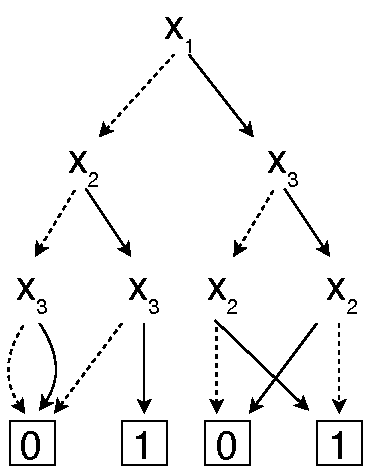
\includegraphics[scale=0.7]{figures/bdd1.pdf}
        \caption{BDD}
        \label{fig:BDD}
    \end{subfigure}%
    \begin{subfigure}[b]{.5\linewidth}
        \centering
        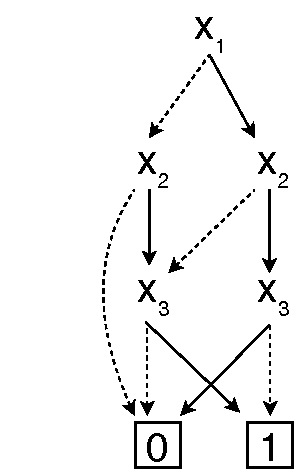
\includegraphics[scale=0.7]{figures/bdd2.pdf}
        \caption{ROBDD}
        \label{fig:ROBDD}
    \end{subfigure}
    \caption{An example of a BDD and an ROBDD representing the same BF $((\neg x_1 \land x_2 \land x_3) \lor (x_1 \land \neg (x_2 \lequal x_3))$}
    \label{fig:BDDandROBDD}
\end{figure}

\begin{example}
\label{ex:BDD}
Figure~\ref{fig:BDD} shows an example of a BDD representing the BF $(\neg x_1 \land x_2 \land x_3) \lor (x_1 \land \neg (x_2 \lequal x_3))$. 
\end{example}

To have simpler and more effective algorithms for BDDs, we actually use \emph{reduced ordered BDDs} (ROBDDs) which are BDDs such that 
\begin{enumerate}
    \item there is some linear order of variables where each path from the root of the BDD to a terminal node complies with it,
    \item there are no isomorphic (``the same looking'') induced subgraphs and
    \item there are no nodes with the same high and low child.
\end{enumerate}
ROBDDs have the nice property that for a given variable order, each BF $\phi$ is represented by exactly one ROBDD~\cite{BDD}. Furthermore, it represents all BFs equivalent to $\phi$. However, the size of two ROBDDs in different variable orders can for the same formula be very different. We can find a formula which in one ordering has an ROBDD representation whose number of nodes is linear to the size of the formula and in a different one it is exponential. The problem of finding the optimal variable ordering is $\NP$-hard~\cite{BDDoptimalorderisNP}, therefore we usually use some heuristics to reduce the size of ROBDDs and we do not look for the perfect order.

\begin{example}
\label{ex:ROBDD}
Figure~\ref{fig:ROBDD} shows an ROBDD which represents the same BF as the BDD from Example~\ref{ex:BDD}. While the BDD from Figure~\ref{fig:BDD} does not have ordered variables, the paths from root to terminals in ROBDD respect the order $x_1,x_2,x_3$. Also, the leftmost path does not contain $x_3$, because both its low and high child ended in $0$. Furthermore, both $x_2$ nodes share an isomorphic subgraphs.
\end{example}

For each operation on BFs (${\land}$, ${\lor}$, ${\neg}$), there is a polynomial-time algorithm for ROBDDs, which can get the resulting ROBDD representing the application of the operation. For example, if we have an ROBDD representing BF $\psi_1$, we can get an ROBDD representing $\neg \psi_1$ by swapping terminal nodes $0$ and $1$. See for example Andersen~\cite{BDDdetails} for more details.

In the following chapters, when we use BDD we actually mean ROBDD.


\section{Quantifier Trees}
\label{sec:QT}
While BDDs are a good representation of BFs, we also need a representation for DQBFs. For this we define \emph{quantifier trees} which can represent DQBFs in NNF.

\begin{definition}
  Let $V$ be a set of variables. A \emph{quantifier tree} \emph{over $V$} is a rooted tree with labelling $l$ which assigns to each non-terminal node an operation ${\diamond} \in \set{{\land},{\lor}}$ and to each terminal node a literal from $V$ (a variable $x \in V$ or its negation), and a prefix mapping $Q$ which maps to each node some DQBF prefix.
\end{definition}

We denote the set of children of node $n$ as $\children{n}$.  A quantifier tree with root $r$ can possibly represent a DQBF $\psi_r$ where:
\begin{itemize}
    \item if $\qtlabel{r} = l_r$ is a literal, then $\psi_r = \prefix{r} \itholds l_r$,
    \item if $\qtlabel{r} = {\diamond}$ with ${\diamond} \in \set{{\land},{\lor}}$ and $\children{r} = \set{n_1,\dots, n_m}$, then $\psi_r = \prefix{r} \itholds \psi_{n_1} \diamond \dots \diamond \psi_{n_m}$ where $\psi_{n_1} \dots \psi_{n_m}$ are DQBFs represented by subtrees rooted in children $n_1,\dots,n_m$.
\end{itemize}
Not all trees represent some DQBF, we restrict ourselves only to the set of quantifier trees which represent some formula. However, for each DQBF there exists a quantifier tree representing it.

For a node $n$, we use $\eprefix{n}$ and $\uprefix{n}$ to denote the set of existentially and universally quantified variables in $\prefix{n}$. The sets $\vars{n}, \evars{n}$ and $\uvars{n}$ denote $\vars{\psi_n}, \evars{\psi_n}$ and $\uvars{\psi_n}$ respectively, where $\psi_n$ is DQBF represented by a subtree rooted in $n$.

In figures, each node $n$ is denoted by its assigned operation or literal $\qtlabel{n}$, while the assigned DQBF prefix $\prefix{n}$ is always shown on the edge coming to it (see Figure~\ref{fig:QTex}). For the root, we add an extra ``edge'' on which we show this quantifier prefix.

\begin{figure}
  \centering
  %\begin{tikzpicture}[->,>={Stealth[scale=1.3,angle'=90]},node distance=2cm,initial distance=1.3cm,initial text=$\forall x_1 \exists y_1(x_1) $,every state/.style={minimum size=2em, inner sep=1pt}]
  %  \node[state,initial above] (1) {${\land}$};
  %  \node[state, below of=1] (2) {$x_1$};
  %  \node[state, left of=2] (3) {${\lor}$};
  %  \node[state, right of=2] (4) {${\lor}$};
  %  \node[state, below right = 1.3cm and 0.4 cm of 4] (5) {$\neg y_1$};
  %  \node[state, below left = 1.3cm and 0.4 cm of 4] (6) {$x_2$};
  %  \node[state, below right = 1.3cm and 0.4cm of 3] (7) {$\neg x_1$};
  %  \node[state, below left = 1.3cm and 0.4cm of 3] (8) {$y_2$};
  %  
  %  \draw (1) edge[right] node{$\forall x_2$} (4)
  %        (1) edge[left] node{$\exists y_2(\emptyset)$} (3)
  %        (1) edge (2)
  %        (3) edge (7)
  %        (3) edge (8)
  %        (4) edge (5)
  %        (4) edge (6)
  %        ;
  %\end{tikzpicture}
    
  \begin{forest}
    [$\forall x_1 \exists y_1(x_1)$, for descendants={circle, draw, minimum size=2em, inner sep=1pt}
      [${\land}$
        [${\lor}$, edge label={node[midway,above left]{$\exists y_2(\emptyset)$}}
          [$y_2$]
          [$\neg x_1$]
        ]
        [$x_1$]
        [${\lor}$, edge label={node[midway,above right]{$\forall x_2$}}
          [$x_2$]
          [$\neg y_1$]
        ]
      ]
    ]
  \end{forest}
  \caption{An example of quantifier tree}
  \label{fig:QTex}
\end{figure}

\begin{example}
  Figure~\ref{fig:QTex} shows an example of quantifier tree representing DQBF \[\forall x_1 \exists y_1(x_1) (\exists y_2(\emptyset) \itholds (y_2 \lor \neg x_1) \land x_1 \land \forall x_2 \itholds (x_2 \lor \neg y_1)).\]
\end{example}

\chapter{Transformations of DQBFs}
\label{chap:quantmanip}
%In this chapter we give some theoretical results for DQBFs in NNF, which show the equisatisfiability of different DQBFs. which can result in their simplification. These results can be then used for developing a DQBF solver which checks whether an input DQBF is satisfiable or not. TODO!!!!!

%For the latter, we give rules for shifting and eliminating quantifiers inside formula. We then use these for developing our solver in Chapter~\ref{chap:algorithm}. 

In this chapter we give theorems showing equisatisfiabilities of some DQBFs in NNF. Such formulas can be replaced with each other, allowing us to push (pull) quantifiers inside (from) the formula (Section~\ref{sec:quantLocalisation}) or eliminate them (Section~\ref{sec:quantElimination}). We use these results in Chapter~\ref{chap:algorithm} to develop an algorithm solving DQBFs.
%\begin{itemize}
%    \item pushing quantifiers inside formula,
%    \item elimination of quantified variables or
%    \item ????removal of universal variables from the dependency sets of existential variables.????
%\end{itemize}



\section{Shifting Quantifiers}
\label{sec:quantLocalisation}
We start with a theorem that shows some rules by which we can push (extract) quantifiers in (from) the formula. 

\begin{theorem}[{\cite[Theorems 3,4]{HQSquantifierLocalisation}}]
\label{thrm:quantLocalEq}
  Let ${\diamond} \in \set{{\land},{\lor}}$ and $\psi,\psi_1,\psi_2 \in \DQBF{V}$. We assume that variables $x$, $x_1$, $x_2$, $y$, $y_1$, and $y_2$ are not quantified in $\psi, \psi_1$, and $\psi_2$. We also assume that $x'$ and $y'$ are fresh variables, which do not occur in $\psi,\psi_1$ and $\psi_2$. Then we have:
  \begin{align}
      %\forall x : \psi &\approx \psi \text{, if } x \not\in V_{\psi} \\
      \forall x \itholds (\psi_1 \land \psi_2) &\approx \left(\forall x \itholds \psi_1 \land \forall x' \itholds \psi_2\substitute{x}{x'}\right) \tag{a} \label{loc:unconj1} \\
      \forall x \itholds (\psi_1 \land \psi_2) &\approx \left(\psi_1^{-x} \land \forall x \itholds \psi_2\right) \text{, if } x \not\in V_{\psi_1} \tag{b} \label{loc:unconj2} \\
      \forall x \itholds (\psi_1 \diamond \psi_2) &\approx \begin{multlined}[t][3cm]\left(\psi_1 \diamond \forall x \itholds \psi_2\right) \text{, if } x \not\in V_{\psi_1} \tag{c} \label{loc:undisj} \\
      \text{ and } x \not\in D_y \text{ for all } y \in \evars{\psi_1}\end{multlined} \\
      \exists y(D_y) \itholds (\psi_1 \lor \psi_2) &\approx \left(\exists y(D_y) \itholds \psi_1 \lor \exists y'(D_y) \itholds \psi_2\substitute{y}{y'}\right) \tag{d} \label{loc:exdisj} \\
      \exists y(D_y) \itholds (\psi_1 \diamond \psi_2) &\approx \left(\psi_1 \diamond \exists y(D_y) \itholds \psi_2\right) \text{, if } y \not\in V_{\psi_1} \tag{e} \label{loc:exboth} \\
      \exists y_1(D_{y_1})\exists y_2(D_{y_2}) \itholds \psi &\approx \exists y_2(D_{y_2}) \exists y_1(D_{y_1}) \itholds \psi \tag{f} \label{loc:exswap} \\
      \forall x_1\forall x_2 \itholds \psi &\approx \forall x_2\forall x_1 \itholds \psi \tag{g} \label{loc:unswap} \\
      \forall x\exists y(D_y) \itholds \psi &\approx \exists y(D_y)\forall x \itholds \psi\text{, if } x \not\in D_y. \tag{h} \label{loc:bothswap}
  \end{align}
\end{theorem}

To make these rules more usable for DQBF in NNF we have to show that they also work while replacing subformulas. Except for~\eqref{loc:unconj2}, this was not proven by Ge-Ernst et al.~\cite{HQSquantifierLocalisation} even though they use them for replacing subformulas. As we will show, this was used erroneously because the rule~\eqref{loc:exdisj} does not generally hold. However, for other rules there is no problem as we show in Theorem~\ref{thrm:quantLocalSubformulas}. But first we give some helpful notions and lemmas we use for the proofs of following theorems.

In the proofs we work with Skolem function mappings, which turn DQBFs to BFs. We will want to show, that some subformulas are ``important'', i.e. changing their evaluation change the evaluation of the whole formula. Therefore we define the notion of dependency of Boolean formula on its subformula.
\begin{definition}
  Let $\phi, \phi' \in \BF{V}$, $v \in \valtns{V}$ and $\phi'$ is subformula of $\phi$. We say that $\phi$ \emph{depends on} $\phi'$ \emph{in} v, if $v(\phi\substitute{\phi'}{0}) \not= v(\phi\substitute{\phi'}{1})$.
\end{definition}
This means that if $\phi$ depends on its subformula $\phi'$ in $v$, the value of $v(\phi)$ would change if the value of $v(\phi')$ was different.

\begin{remark}
  If $v(\phi') = 1$ then $v(\phi) = v(\phi\substitute{\phi'}{1})$ and if $v(\phi') = 0$ then $v(\phi) = v(\phi\substitute{\phi'}{0})$.
\end{remark}

The first lemma we prove shows that if the subformula $\phi'$ occurs in the tree of operations in $\phi$ without negation anywhere before it, then $v(\phi) = v(\phi')$.
\begin{lemma}
  \label{lemma:nonegdepends}
  Let $\phi, \phi' \in \BF{V}$, $v \in \valtns{V}$ where $\phi'$ is subformula of $\phi$ and $\phi$ depends on $\phi'$ in $v$. Assume that for each subformula $\neg \phi''$ of $\phi$ we have that $\phi'$ is not subformula of $\phi''$. Then $v(\phi) = v(\phi')$.
\end{lemma}
\begin{proof}
  From assumptions, it holds that $\phi'$ is only in conjunctions and disjunctions in the tree of operations. Therefore it has to hold that if $v(\phi\substitute{\phi'}{0}) = 1$ then also $v(\phi\substitute{\phi'}{1}) = 1$. But because $\phi$ depends on $\phi'$ in $v$, this cannot be, which means that $v(\phi\substitute{\phi'}{0}) = 0$ and $v(\phi\substitute{\phi'}{1}) = 1$. This means that $v(\phi) = v(\phi')$.
\end{proof}

Next, we prove a lemma that says that if $\phi$ depends on its subformula $\phi'$ in a valuation $v$, then $\phi$ also depends on $\phi'$ in a valuation $v'$, which differs from $v$ only in the variables that do not occur outside $\phi'$.
\begin{lemma}
  \label{lemma:dependschangedval}
  Let $\phi, \phi' \in \BF{V}$, $v \in \valtns{V}$ where $\phi'$ is subformula of $\phi$ and $\phi$ depends on $\phi'$ in $v$. Let $v' \in \valtns{V}$ be a valuation where $v'(x) = v(x)$ for every $x$ occurring outside the subformula $\phi'$. Then $\phi$ depends on $\phi'$ in $v'$.
\end{lemma}
\begin{proof}
  Because we can only change the values of variable inside $\phi'$, it still holds that $v'(\phi\substitute{\phi'}{1}) = v(\phi\substitute{\phi'}{1})$ and $v'(\phi\substitute{\phi'}{0}) = v(\phi\substitute{\phi'}{0})$. Then, from the fact that $\phi$ depends on $\phi'$ in $v$, we have $v'(\phi\substitute{\phi'}{1}) = v(\phi\substitute{\phi'}{1}) \not= v'(\phi\substitute{\phi'}{0}) = v(\phi\substitute{\phi'}{0})$ which means that $\phi$ depends on $\phi'$ in $v'$.
\end{proof}

\begin{theorem}
  \label{thrm:quantLocalSubformulas}
  Let $\phi$ be the left side formula and $\phi'$ be the right side formula of the same equisatisfiability other than~\eqref{loc:exdisj} from Theorem~\ref{thrm:quantLocalEq}. Let $\psi \in \DQBF{V}$ such that $\phi$ is a subformula of $\psi$ and $\psi'$, which results from $\psi$ by replacing $\phi$ with $\phi'$, is a valid DQBF. Then $\psi \approx \psi'$.
\end{theorem}
\begin{proof}
  \eqref{loc:unconj1} $\phi = \forall x \itholds (\psi_1 \land \psi_2)$ and $\phi' = \left(\forall x \itholds \psi_1 \land \forall x' \itholds \psi_2\substitute{x}{x'}\right)$
  
  We show that $\seman{\psi} \not= \emptyset$ iff $\seman{\psi'} \not= \emptyset$. First, let $s \in \seman{\psi}$. We now show that for $s'$, where 
  \begin{itemize}
      \item $s'(y) = s(y)\substitute{x}{x'}$\footnote{By $s(y)\substitute{x}{x'}$ we mean the BF representing $s(y)$ in which every occurrence of $x$ is replaced by $x'$ and to $s(y')$ we assign Boolean function that $s(y)\substitute{x}{x'}$ represents} for $y \in \evars{\psi_2}$ and
      \item $s'(y) = s(y)$ otherwise,
  \end{itemize}
  it holds $s' \in \seman{\psi'}$. Note that for $y \in \evars{\psi_1}$ we have $s'(y) = s(y)$ as, according to the way DQBFs are defined, $\psi_1$ and $\psi_2$ cannot share the same quantification, therefore $\evars{\psi_1} \cap \evars{\psi_2} = \emptyset$.
  
  Let $v \in \valtns{\uvars{\psi'}}$. We need to show that $v(s'(\psi')) = 1$. Because $s \in \seman{\psi}$, it holds that $v(s(\psi)) = 1$. For the case that $v(x') = v(x)$ we get $v(s(\psi)) = v(s'(\psi'))$, because BFs $s(\psi)$ and $s(\psi')$ differ only in some replacements of $x$ by $x'$. Therefore we assume that $v(x') \not= v(x)$. We know that $\psi$ and $\psi'$ differ only in the formulas $\phi$ and $\phi'$, therefore we can only focus on the case where $s(\psi)$ depends on $s(\phi)$ in $v$ (otherwise $v(s(\psi)) = v(s'(\psi'))$). %(that is the value of $v(s(\psi))$ would change if the value of $v(s(\phi))$ changed). 
  Also, $\psi$ is in NNF, which means that in the tree of operations, negation cannot be before $\phi$. We can then apply Lemma~\ref{lemma:nonegdepends} and we get $v(s(\phi)) = 1$.
  This means we need to show that $v(s'(\phi')) = 1$.
  
  We have that for $v(s(\phi)) = v(s(\forall x \itholds (\psi_1 \land \psi_2))) = v(s(\psi_1) \land s(\psi_2))$ to be equal to one, it has to hold that $v(s(\psi_1)) = 1$ and $v(s(\psi_2)) = 1$. Also, for $v'$ which is equal to $v$, except that $v'(x) \not= v(x)$, it holds that $v'(s(\psi)) = 1$ (from $s \in \seman{\psi}$). Because $x$ is not outside $s(\phi)$, we can use Lemma~\ref{lemma:dependschangedval} to see that $\psi$ depends on $\phi$ in $v'$ too, and by applying Lemma~\ref{lemma:nonegdepends} we get $v'(s(\phi)) = 1$.
  %This is from the assumption that the value of $v(s(\psi))$ depends on $v(s(\phi))$, because $x$ is only in $\phi$. 
  This means that $v'(s(\psi_2)) = 1$. Also $v'(s(\psi_2)) = v(s'(\psi_2\substitute{x}{x'}))$, because $v'(x) = v(x')$. All in all, we get $v(s(\psi_1)) = v(s'(\psi_1)) = 1$ and $v(s'(\psi_2\substitute{x}{x'})) = 1$ therefore $v(s'(\phi')) = v(s'(\forall x \itholds \psi_1 \land \forall x' \itholds \psi_2\substitute{x}{x'})) = v(s'(\psi_1) \land s'(\psi_2\substitute{x}{x'})) = 1$.
  
  For the other direction, let $s' \in \seman{\psi'}$. It can be easily shown by similar argument that $s$, where $s(y) = s'(y)\substitute{x'}{x}$ for $y \in \evars{\psi_2}$ and $s(y) = s'(y)$ otherwise, is a satisfying Skolem functions mapping of $\psi$.
  
  \eqref{loc:unconj2} This was proven by Ge-Ernst et al.~\cite[Theorem 4]{HQSquantifierLocalisation}.
  
  \eqref{loc:undisj}\eqref{loc:exboth}\eqref{loc:exswap}\eqref{loc:unswap}\eqref{loc:bothswap} Because $\uvars{\psi} = \uvars{\psi'}$, $\evars{\psi} = \evars{\psi'}$, and $\fvars{\psi} = \fvars{\psi'}$ and the dependency sets do not change, it holds that $\Scands{\psi} = \Scands{\psi'}$. Also, for any $s \in \Scands{\psi}$ it holds that $s(\psi)$ is the same BF as $s(\psi')$ which means that $\seman{\psi} = \seman{\psi'}$, therefore $\psi \approx \psi'$.
\end{proof}

As we already mentioned, the rule~\eqref{loc:exdisj} as it stands cannot be generally used for replacing subformulas. We show it on the following formula:
\[\forall x \exists y(\emptyset) \itholds ((x \land y) \lor (\neg x \land \neg y)).\]

It is obviously not satisfiable because whether $s(y) = 0$ or $s(y) = 1$ we can always find valuation in which both disjuncts are not true. However if we assumed that the rule~(\ref{loc:exdisj}) can be also used for subformulas, we would get
\[\forall x \itholds (\exists y(\emptyset) \itholds (x \land y) \lor \exists y'(\emptyset) \itholds (\neg x \land \neg y')),\]
which is satisfiable for $s$ where $s(y) = 1$ and $s(y') = 0$. To fix this, we need to restrict the variables that can occur in the disjuncts. When we look at this formula, it would appear that the problem arises from having universal variable $x$ on which $y$ is not dependent in both disjuncts. However, we can find an example when even if both disjuncts contain different sets of universal variables (other than the ones from $D_y$), this rule does not work. For example for unsatisfiable formula
\[\forall x_1 \forall x_2 \itholds (\exists y(\emptyset) \itholds ((x_1 \land y) \lor (x_2 \land \neg y)) \lor (\neg x_1 \land \neg x_2)),\]
we have that $(x_1 \land y)$ contains $x_1$, which is not in $(x_2 \land \neg y)$. and $x_2$ is only in the second disjunct. However, after applying the rule~\eqref{loc:exdisj} we get
\[\forall x_1 \forall x_2 \itholds ((\exists y(\emptyset) \itholds (x_1 \land y) \lor \exists y'(\emptyset) \itholds (x_2 \land \neg y')) \lor (\neg x_1 \land \neg x_2)),\]
which becomes satisfiable. The problem here is that $x_1$ and $x_2$ are in $(\neg x_1 \land \neg x_2)$, which is outside the subformula we are applying the rule $\eqref{loc:exdisj}$ on. Therefore, we can put in a condition that the sets of universal variables (except the ones from $D_y$) from the disjuncts are disjoint and, as the next theorem shows, it is enough that universal variables from one of these disjuncts are not outside this subformula. We also need to not only look at the universal variables occurring in the disjuncts, but also at the ones from the dependency sets of existential variables occurring in the disjuncts.

\begin{theorem}
  \label{thrm:localisedijunction}
  Let $\psi,\psi_1,\psi_2 \in \DQBF{V}$ such that $\exists y(D_y) \itholds (\psi_1 \lor \psi_2)$ is a subformula of $\psi$ and $y'$ be a fresh variable not occurring in $\psi$. Let 
  \[A_{\psi_1} = \Set{x \in \uvars{\psi} \setminus D_y | x \in \vars{\psi_1} \text{ or } x \in D_{y_1} \text{ for some } y_1 \in \vars{\psi_1} \cap \evars{\psi}}\]
  and 
  \[A_{\psi_2} = \Set{x \in \uvars{\psi} \setminus D_y | x \in \vars{\psi_2} \text{ or } x \in D_{y_2} \text{ for some } y_2 \in \vars{\psi_2} \cap \evars{\psi}}.\] 
  Assume that $A_{\psi_1} \cap A_{\psi_2} = \emptyset$ and each variable $x$ from $A_{\psi_1}$ can only occur in $\psi$ outside the subformula $\exists y(D_y) \itholds (\psi_1 \lor \psi_2)$ as quantification $\forall x$ or in a dependency set, but not in the dependency set of any existential variable in $\psi$ that occurs outside the subformula. Then $\psi \approx \psi'$ where $\psi'$ results from $\psi$ by replacing the subformula $\exists y(D_y) \itholds (\psi_1 \lor \psi_2)$ by \[\left(\exists y(D_y) \itholds \psi_1 \lor \exists y'(D_y) \itholds \psi_2\substitute{y}{y'}\right).\]
\end{theorem}
\begin{proof}
  We prove that $\seman{\psi} \not= \emptyset$ iff $\seman{\psi'} \not= \emptyset$. Let $\phi = \exists y(D_y) \itholds (\psi_1 \lor \psi_2)$ and $\phi' = (\exists y(D_y) \itholds \psi_1 \lor \exists y'(D_y) \itholds \psi_2\substitute{y}{y'})$. 
  
  First, let $s \in \seman{\psi}$. It is easy to see that $s'$, where $s'(y') = s(y)$ and for other variables it maps to the same Skolem function as $s$, is a satisfying Skolem functions mapping of $\psi'$, because $s(\psi)$ and $s(\psi')$ are the same BFs.
  
  Now, assume that $s' \in \seman{\psi'}$. In the rest of the proof, for every valuation $v \in \valtns{\uvars{\psi}}$ (where it also holds that $v \in \valtns{\uvars{\psi'}}$, because $\uvars{\psi} = \uvars{\psi'}$) we use $v_{D_y}$ to denote the restriction of $v$ to $D_y$. Let $s$ be a Skolem function mapping of $\psi$ such that for $v \in \valtns{\uvars{\psi}}$ 
  \begin{itemize}
      \item $s(y)(v) = s'(y)(v)$ if for all valuations $v' \in \valtns{\uvars{\psi}}$, for which it holds that $v'_{D_y} = v_{D_y}$ and $s'(\psi')$ depends on the subformula $s'(\phi')$ in $v$, we have $v(s'(\psi_1)) = 1$,
      \item $s(y)(v) = s'(y')(v)$ otherwise.
  \end{itemize}
  For other variables, $s$ maps to the same Skolem function as $s'$. We show that $s \in \seman{\psi}$.
  
  Let $v \in \valtns{\uvars{\psi}}$ be a valuation. We need to show that $v(s(\psi)) = 1$. With similar reasoning as in the proof of case~\eqref{loc:unconj1} of Theorem~\ref{thrm:quantLocalSubformulas}, we can assume that $s'(\psi')$ depends on the subformula $s'(\phi')$ in $v$ and $v(s'(\phi')) = 1$. Because the only difference between $s(\psi)$ and $s'(\psi')$ is in subformulas $s(\phi)$ and $s'(\phi)$, we only need to show that $v(s(\phi)) = 1$.
  
  Because 
  \[s'(\phi') = s'(\exists y(D_y) \itholds \psi_1 \lor \exists y'(D_y) \itholds \psi_2\substitute{y}{y'}) = s'(\psi_1) \lor s'(\psi_2\substitute{y}{y'})\] is a disjunction, it has to hold that $v(s'(\psi_1)) = 1$ or $v(s'(\psi_2\substitute{y}{y'})) = 1$.
  If they are both equal to 1, then it does not matter whether $s(y)(v) = s'(y)(v)$ or $s(y)(v) = s'(y')(v)$, it will always hold that $v(s(\phi)) = 1$.
  If we have $v(s'(\psi_1)) = 0$ and $v(s'(\psi_2\substitute{y}{y'})) = 1$, then from the definition of $s$, we get $s(y)(v) = s'(y')(v)$ and so $v(s(\psi_2)) = v(s(\psi_2\substitute{y}{y'})) = 1$ and therefore $v(s(\phi)) = 1$.
  
  For the last case, $v(s'(\psi_1)) = 1$ and $v(s'(\psi_2\substitute{y}{y'})) = 0$, we need to show that $s(y)(v) = s'(y)(v)$, because then $v(s(\psi_1)) = v(s'(\psi_1)) = 1$ therefore $v(s(\phi)) = 1$. For that, we need to show that for each valuation $v' \in \valtns{\uvars{\psi}}$ where $v'_{D_y} = v_{D_y}$ and $s'(\psi')$ depends on $s'(\phi')$ in $v$, it holds $v'(s'(\psi_1)) = 1$. Assume that this does not hold meaning that there exists some $v'$ fulfilling these conditions where $v'(s'(\psi_1)) = 0$. We now show contradiction.
  
  Let $v'' \in \valtns{\uvars{\psi}}$ be a valuation such that $v''(x) = v'(x)$ for all $x \in A_{\psi_1}$ and $v''(x) = v(x)$ otherwise. This means that $v''_{D_y} = v_{D_y} = v'_{D_y}$. Because $s'(\psi_1)$ contains only variables from $A_{\psi_1} \cup D_y$ we have $v''(s'(\psi_1)) = v'(s'(\psi_1)) = 0$. Moreover, because $A_{\psi_1} \cap A_{\psi_2} = \emptyset$ (from the assumption of the theorem) and $s'(\psi_2\substitute{y}{y'})$ contains only variables from $A_{\psi_2} \cup D_y$, we have $v''(s'(\psi_2\substitute{y}{y'})) = v(s'(\psi_2\substitute{y}{y'})) = 0$. Together, this means $v''(s'(\phi')) = 0$.
  
  Furthermore, because variables from $A_{\psi_1}$ are not ``outside'' the subformula $s'(\phi')$ (from the assumption of the theorem) and all the ``outside'' variables are set to the same value as $v$, we can use Lemma~\ref{lemma:dependschangedval} to show that $s'(\psi')$ depends on the subformula $s'(\phi')$ in $v''$ (as was the case for $v$). However, because $\psi'$ is in NNF and so $s'(\phi')$ does not have negation anywhere in front of it, we can use Lemma~\ref{lemma:nonegdepends} to show that $v''(s'(\phi')) = v''(s'(\psi')) = 1$ (because $s' \in \seman{\psi'}$) which is a contradiction.
\end{proof}

\begin{remark}
  The condition that variables from $A_{\psi_1}$ cannot occur outside the subformula $\exists y(D_y) \itholds (\psi_1 \lor \psi_2)$ can be replaced with the same condition for $A_{\psi_2}$. The proof would then have just a minor differences.
\end{remark}

\section{Quantifier Elimination}
\label{sec:quantElimination}
In this section we show how we can eliminate both universal and existential quantifiers. Firstly, we show that for a simple case where the quantified variable is not in the formula, we can just remove it.

\begin{lemma}
\label{lemma:elimination}
Let $\psi_1 \in \DQBF{V}$. Assume that variables $x$ and $y$ are not quantified in $\psi_1$ and $y$ is not in any dependency set in $\psi_1$. Then
\begin{align}
    \forall x \itholds \psi_1 &\approx \psi_1^{-x} \text{, if } x \not\in \vars{\psi_1}\tag{i}\label{elim:univ}\\
    \exists y(D_y) \itholds \psi_1 &\approx \psi_1 \text{, if } y \not\in \vars{\psi_1}.\tag{j}\label{elim:exist}
\end{align}
Let $\psi \in \DQBF{V}$ be a formula such that the left side of one of the previous equisatisfiabilities is its subformula. Then $\psi \approx \psi'$ where $\psi'$ results from $\psi$ by replacing this subformula with the equisatisfiable right side.
\end{lemma}
\begin{proof}
  We show the general case $\psi \approx \psi'$ for both equisatisfiabilities.
  
  \eqref{elim:univ} Again, we want to prove $\seman{\psi} = \seman{\psi'}$. For $s \in \seman{\psi'}$ it is obvious that also $s \in \seman{\psi}$. For $s \in \seman{\psi}$ we can create $s'$ where $s'(y) = s_{x=0}(y)$ where $s_{x=0}(y)$ is a Boolean function that behave like $s_y$ where $x$ is set to $0$. Then $s' \in \seman{\psi'}$ because for each valuation $v \in \valtns{\uvars{\psi}}$ where $v(x) = 0$, we have $v(s'(\psi')) = v(s(\psi)) = 1$.
  
  \eqref{elim:exist} Stems from the fact that $s(\psi)$ and $s(\psi')$ are the same BF for any $s \in \Scands{\psi}$.
\end{proof}

The next theorem shows how to eliminate universal quantifiers generally by universal expansion. This can be always applied to any universal quantifier but by doing so the resulting DQBF can contain new copies of existential variables. The theorem is based on universal expansion for DQBFs in PNF~\cite{HQSsimpleAlg,NegationOfDQBFs}, here we generalise it to the case of subformulas in DQBFs in NNF.

\begin{theorem}[Universal Expansion]
\label{thrm:unExpan}
  Let $\psi, \psi_1 \in \DQBF{V}$ such that $\forall x \itholds \psi_1$ is a subformula of $\psi$ where $\psi_1$ does not include any quantifications other than the ones bounded to variables from the set $E_{x} = \set{y \in \evars{\psi} | x \in D_y}$ of all existential variables dependent on $x$. Let $\psi_2$ be a DQBF that results from $\psi_1$ by substituting each $y \in E_x$ with a fresh variable $y'$ not occurring in $\psi$ where we set $D_{y'} = D_y$. Then $\psi \approx \psi'$ where $\psi'$ results from $\psi$ by replacing the subformula $\forall x \itholds \psi_1$ by 
  \[\xi = (\psi_1^{-x}\substitute{x}{0} \land \psi_2^{-x}\substitute{x}{1}).\]
\end{theorem}
\begin{proof}
  Note that each $y \in E_x$ must be entirely inside $\psi_1$ (even the ``$\exists y$'' bit). This stems from the way the set $\DQBF{V}$ is constructed; the dependency sets of new existential variables can only be formed from free or completely new variables and if ``$\exists y$'' was outside $\forall x \itholds \psi_1$, then $x \in D_y$ would have to be a free or new variable. Also, because of the assumption that only quantifiers bounded to existential variables from $E_x$
  are in $\psi_1$ it is obvious that $\psi' \in \DQBF{V}$. With that we can now prove that $\seman{\psi} \not= \emptyset$ iff $\seman{\psi'} \not= \emptyset$.
  
  First we prove that if $\seman{\psi} \not= \emptyset$, then $\seman{\psi'} \not= \emptyset$. Let $s \in \seman{\psi}$. We build a satisfying Skolem functions mapping $s'$ of $\psi'$. For $y \in E_x$ and its copy $y' \in \evars{\psi_2}$ we set $s'(y) = s_{x=0}(y)$ and $s'(y') = s_{x=1}(y)$ where $s_{x=0}(y)$ and $s_{x=1}(y)$ denote Boolean functions that behave like $s(y)$ where $x$ is set to $0$ or $1$ respectively. Otherwise we set $s'(y) = s(y)$. Then $s'$ is a Skolem functions mapping of $\psi'$.
  
  To show that it is satisfying, we have to prove that BF $s'(\psi')$ is true in all valuations over $\uvars{\psi'}$. Notice that $\uvars{\psi'} = \uvars{\psi} \setminus \set{x}$. Let $v$ be one such valuation and denote $v_{x\mapsto0}$ and $v_{x\mapsto1}$ valuations over $\uvars{\psi}$ such that $v(x') = v_{x\mapsto0}(x') = v_{x\mapsto1}(x')$ for $x' \in \uvars{\psi'}$, $v_{x\mapsto0}(x) = 0$ and $v_{x\mapsto1}(x) = 1$. It holds that $v_{x\mapsto0}(s(\forall x\itholds\psi_1)) = v(s'(\psi_1^{-x}\substitute{x}{0}))$ and $v_{x\mapsto1}(s(\forall x\itholds\psi_1)) = v(s'(\psi_2^{-x}\substitute{x}{1})$.
  
  Therefore, if $v_{x\mapsto0}(s(\forall x\itholds\psi_1)) = v_{x\mapsto1}(s(\forall x\itholds\psi_1)) = \kappa$, where $\kappa \in \set{0,1}$, then $v(s'(\xi)) = \kappa$. If $v_{x\mapsto0}(s(\forall x\itholds\psi_1)) \not= v_{x\mapsto1}(s(\forall x\itholds\psi_1))$ then $v(s'(\xi)) = 0$ where either $v_{x\mapsto0}(s(\forall x\itholds\psi_1)) = 0$ or $v_{x\mapsto1}(s(\forall x\itholds\psi_1)) = 0$. This means that $v(s'(\xi))$ is equal to $v_{x\mapsto0}(s(\forall x\itholds\psi_1))$ or $v_{x\mapsto1}(s(\forall x\itholds\psi_1))$. Also, because $s \in \seman{\psi}$, it has to hold that $v_{x\mapsto0}(s(\psi)) = v_{x\mapsto1}(s(\psi)) = 1$. Furthermore, the only difference in $s(\psi)$ and $s(\psi')$ are the subformulas $s(\forall x\itholds\psi_1)$ and $s'(\xi)$. This all means that $v(s'(\psi')) = 1$.

  Now we prove the other direction. Let $s' \in \seman{\psi'}$. We build a satisfying Skolem functions mapping $s$ of $\psi$. For $y \in E_x$ with a copy $y' \in \evars{\psi_2}$ we set $s(y)$ to Boolean function that is represented by BF $((\neg x \land s'(y)) \lor (x \land s'(y')))$ where $s'(y)$ and $s'(y')$ are replaced with BFs representing them. Otherwise we set $s(y) = s'(y)$. It is obviously a Skolem functions mapping, thus we need to prove that $s(\psi)$ is true in all valuations. Let $v$ be a valuation over $\uvars{\psi}$. Without loss of generality assume that $v(x) = 0$. Then $v(s(y)) = v(s'(y))$. This means that $v(s(\forall x \itholds \psi_1)) = v(s(\psi_1^{-x}\substitute{x}{0}))$. Again we show that $v(s(\psi)) = 1$ from the facts that $v(s'(\psi')) = 1$ (because $s' \in \seman{\psi'}$) and that the only difference in $s(\psi)$ and $s(\psi')$ are the subformulas $s(\forall x\itholds\psi_1)$ and $s'(\xi)$. If $v(s'(\xi)) = 1$ then $v(s(\forall x \itholds \psi_1)) = v(s'(\psi_1^{-x}\substitute{x}{0}) = 1$ and from the previous facts it means that $v(s(\psi)) = 1$. For the case when $v(s'(\xi)) = 0$ we have to realise that because $\psi'$ is in NNF, $s'(\xi)$ occurs in $s'(\psi')$ in a tree of ${\land}$ and ${\lor}$ operations. That means that even if we replaced $s'(\xi)$ with $s(\forall x \itholds \psi_1)$ and $v(s(\forall x \itholds \psi_1)) = 1$, this cannot change the value of the resulting formula $v(s(\psi))$ from $1$ to $0$, therefore $v(s(\psi)) = 1$.
\end{proof}
\begin{example}
Let
\[\psi = \forall x_1 \forall x_2\itholds ((x_1 \lequal x_2) \lor \exists y (x_2)\itholds \neg(x_1 \lequal y)).\]
be the DQBF from Example~\ref{ex:DQBF:NNF}. Using universal expansion we can transform it to
\begin{multline*}
    \psi' = \forall x_1 \itholds ((x_1 \lequal 0) \lor \exists y (\emptyset) \neg(x_1 \lequal y)) \land {}\\
    ((x_1 \lequal 1) \lor \exists y' (\emptyset)\itholds\neg(x_1 \lequal y'))
\end{multline*}
which (like $\psi$) is satisfiable.
\end{example}

The conditions when existential elimination is possible are more strict. We can eliminate an existential variable $y$ from subformula $\exists y (D_y) \itholds \psi_1$ of $\psi$ only if $\psi_1$ is quantifier free and universal variables occurring in $\psi_1$ or in dependency sets of existential variables in $\psi_1$ are all in $D_y$.

\begin{theorem}[{\cite[Theorem 5]{HQSquantifierLocalisation}}]
\label{thrm:exElim}
  Let $\psi, \psi_1 \in \DQBF{V}$ such that $\exists y(D_y)\itholds\psi_1$ is a subformula of $\psi$ where $\psi_1$ does not include any quantification and includes only variables from $D_y \cup \fvars{\psi} \cup \set{y' \in \evars{\psi} | D_{y'} \subseteq D_y}$. Then $\psi \approx \psi'$ where $\psi'$ results from $\psi$ by replacing the subformula $\exists y(D_y)\itholds\psi_1$ by
  \[(\psi_1\substitute{y}{0} \lor \psi_1\substitute{y}{1}).\]
\end{theorem}
%The condition ... is there so that the replaced subformula stays a proper DQBF.
\begin{example}
Let
\begin{multline*}
\psi = \forall x_1 \forall x_2 \exists y_1(x_1) \itholds (((x_1 \land x_2) \lequal y_1) \lor {} \\
\exists y_2 (x_1,x_2) \itholds ((x_1 \lequal y_2) \land (y_1 \lequal y_2)))
\end{multline*}
be a DQBF that says that either $y_1$ has the same value as $x_1 \land x_2$ (which is impossible because $y_1$ depends only on $x_1$) or there is some $y_2$ which is equal to both $y_1$ and $x_1$ (which is possible because both $y_1$ and $y_2$ depend on $x_1$). This means that this formula is satisfiable. Because the subformula $\exists y_2 (x_1,x_2) \itholds (x_1 \lequal y_2) \land (y_1 \lequal y_2)$ fulfills the conditions from the theorem, $\psi$ can be transformed to
\begin{multline*}
\psi = \forall x_1 \forall x_2 \exists y_1(x_1) \itholds (((x_1 \land x_2) \lequal y_1) \lor {}\\
(((x_1 \lequal 0) \land (y_1 \lequal 0)) \lor ((x_1 \lequal 1) \land (y_1 \lequal 1))))
\end{multline*}
which is still satisfiable.
\end{example}



\chapter{State of the Art}
\label{chap:SoA}
In this chapter, we give an overview of existing solutions and solvers for the satisfiability problem of DQBF. Because there are already multiple surveys about DQBF~\cite{DQBFStateOfArtTalk,DQBFStateOfArt,DQBFStateOfArtNew}, we give only a short overview of most solvers and techniques. However, we go into more details for the solver HQS, because it is currently the best performing solver (winner of the DQBF track of the QBF Evaluation 2018~\cite{QBFeval18} and 2019~\cite{QBFeval19}) and the methods we use for developing our solver are based on the workings of this solver.

\section{First Solution -- DQDPLL}
The first solver that tackled the satisfiability problem for DQBF was based on the DPLL algorithm~\cite{DPLL} which is successfully used for BF and QBF solvers. This algorithm works on Boolean formulas in CNF by searching for a satisfying assignment based on the clauses in CNF. By recursively choosing an assignment for literals and checking whether the remaining clauses contain an empty one (which implies unsatisfiability), DPLL searches trough all assignments until a satisfying one is found or all of them are decided to be unsatisfying. An adaptation called DQDPLL~\cite{DPLLalgorithm} was introduced for DQBF (in PCNF) which extended existing solutions for QBF by adding so-called Skolem clauses which encode the dependencies between existential and universal variables. However, by doing so the algorithm becomes too slow and results in an uncompetitive solver.

\section{Instantiation -- iDQ and iProver}
The first efficient DQBF solver, called iDQ~\cite{iDQandDQDIMACS}, is based on an instantiation technique used for solving \emph{Effectively Propositional Logic} (EPR)~\cite{iProver}. This solver also works only on formulas in PCNF where in each step of the algorithm it tries to create a BF $\phi$ that is an overapproximation of an input DQBF. This is done by instantiating some set of clauses, that is it applies universal expansion locally to them. This BF $\phi$ is then checked for satisfiability, where if $\phi$ is unsatisfiable then the input DQBF is also not satisfiable, while if it is satisfiable, it must be checked if the resulting valuation is valid for the input DQBF. If it is not, then it is used to create more clause instances which are then used to refine this overapproximation.

Furthermore, a solver for EPR can also be used directly for DQBF. Because EPR belongs to the same complexity class as DQBF, there exists a polynomial-time reduction from DQBF to EPR~\cite{iDQandDQDIMACS}. This is used by EPR solver iProver~\cite{iProver} which transforms a DQBF in PCNF to an EPR instance and then solves this.

\section{Clausal Abstraction -- dCAQE}
Another DQBF solver called dCAQE~\cite{dCAQE} is based on clausal abstraction~\cite{ClausalAbstr}. This solver --- working again on DQBF in PCNF --- first puts universally and existentially quantified variables to some sets (called nodes) which are then divided into levels based on the ordering of dependencies of existential variables. The algorithm then constructs for each node on each level a BF that represents which clauses in CNF it can satisfy (for existential node) or falsify (for universal node). The algorithm then builds a candidate valuation by processing each level. For each level either this valuation is extended, or there is some conflict which means that the algorithm has to backtrack to some lower level and refine the abstraction, or the candidate valuation is a satisfying one which ends the algorithm.

\section{Quantifier Elimination -- HQS}
The next solver is based on quantifier elimination. This solver's basic premise is simple --- it iteratively chooses some universal variable for universal expansion (Theorem~\ref{thrm:unExpan}) thus eliminating it and then eliminates all existential quantifiers that are dependent on all leftover universal quantifiers using Theorem~\ref{thrm:exElim}.

\begin{algorithm}
\caption{Quantifier elimination algorithm}
\label{alg:QE}
\begin{algorithmic}[1]
\Function{SolveDQBF}{DQBF $\psi$ in PCNF}
\While{$\uvars{\psi}$ is not empty}%there is some universal variable $x$ in $\psi$
    \State choose $x$ from $\uvars{\psi}$
    \State $\psi = \forall\text{-expansion}(x,\psi)$ \Comment{Theorem~\ref{thrm:unExpan}}% universal expansion
    \ForAll{$y \in \evars{\psi}$ s. t. $D_y = \uvars{\psi}$} %existential variables $y$ such that they depend on all universal variables in $\psi$
        \State $\psi = \exists\text{-elimination}(y,\psi)$ \Comment{Theorem~\ref{thrm:exElim}}% existential expansion
        %\State remove $y$ from $\evars{\psi}$
    \EndFor
\EndWhile
\State return SAT($\psi$)
\EndFunction
\end{algorithmic}
\end{algorithm}

Gitina et al.~\cite{HQSsimpleAlg} introduced the basic algorithm for solving DQBF in PCNF in this way. Algorithm~\ref{alg:QE} shows simple pseudocode of this. In every step, this algorithm chooses (using some heuristic) an universal variable to eliminate. The authors used a heuristic where the universal variable is chosen based on the number of existential ones that depend on it --- they choose the one that has minimal number of dependencies. After that, all the existential variables that depend on everything are also eliminated. To use this algorithm it is important to choose a good representation of the matrix of the DQBF. For this the authors chose and-inverter graphs~\cite{FRAIGs}. % (AIG) which are tree-like structures where non-terminal nodes represent conjunction, terminal nodes are variables and these are connected with two types of nodes: normal ones and those that represent negation. With a proper implementation of operations they can be optimised in such a way that they reuse parts of the graphs resulting in functionally reduced AIGs~\cite{FRAIGs}.

Following this technique, solver HQS was introduced~\cite{HQSquantifierElimination} which was enhanced by using QBF solver as a subprocedure. They still eliminate quantifiers in a similar fashion but now they do it until the formula can be transformed to QBF (that is the dependency sets are linearly ordered). On this QBF they then run already existing solver for QBF called AIGSolve~\cite{AIGSolve} which can use more effective techniques developed for QBFs. Universal quantifiers to eliminate are chosen in the beginning in such a way that the number of universal eliminations is as small as possible while still the resulting formula is QBF. For this they build a dependency graph in which nodes are existential variables where $y_i$ is connected to $y_j$ if for their dependency sets it hold that $D_{y_i} \not\subseteq D_{y_j}$. They noticed that if this graph is acyclic, the formula can be seen as QBF. Furthermore, there is a cycle in this graph iff there is a simple cycle (between two nodes) in the graph. They use this to create an instance of MaxSAT problem which is a problem of finding a valuation of one BF while maximizing another formula. This instance then encodes which universal variables have to be eliminated so the dependency graph becomes acyclic while minimising the number of universal variables to eliminate. After finding the set of variables to eliminate, they follow with an improved quantifier elimination algorithm. They also improved it by adding a preprocessing step (see Section~\ref{sec:preprocessing}) and elimination of special types of variables called unit and pure. 

The algorithm was changed a bit again by Wimmer et al.~\cite{HQSdependencyElimination}. The authors were interested in whether it is possible to somehow remove specific dependencies from the list of dependencies of existential variable. They have shown that it is possible, albeit at the expense of adding a new existential variable. This is similar to the universal expansion (Theorem~\ref{thrm:unExpan}), but by removing just one dependency we add just one new existential variable. Let for example
\[\psi = \forall x_1 \dots \forall x_n \exists y_1(D_{y_1}) \dots \exists y_m(D_{y_m}) \itholds \phi\]
be a prenex DQBF where $\phi$ is a BF and $x_1 \in D_{y_1}$. We can now remove $x_1$ from $D_{y_1}$ by adding a copy of $y_1$ resulting in an equisatisfiable DQBF
\begin{multline*}
\forall x_1 \dots \forall x_n \exists y_1^0(D_{y_1} \setminus \{x_1\}) \exists y_1^1(D_{y_1} \setminus \{x_1\}) \exists y_2(D_{y_2})\dots \exists y_m(D_{y_m}) \\
\phi\left[((\neg x_1 \land y_1^0) \lor (x_1 \land y_1^1))/y_1\right].
\end{multline*}
Using this the authors do not look for a set of universal variables to eliminate, but for partial dependencies whose removal will result in a DQBF which can be transformed into QBF. Again, they create a dependency graph which is acyclic iff DQBF can be seen as QBF. But now they create a bipartite graph whose two sets of nodes are the set of universal variables and the set of existential variables which are connected based on whether universal variable is in the dependency set of existential one. Similarly to previous, they use this graph to solve an optimization problem that encodes which dependencies to remove to get QBF which can then be solved with AIGSolve.

Last but not least, Ge-Ernst et al.~\cite{HQSquantifierLocalisation} have given a theoretical foundations for non-prenex DQBFs and the possibility to push and eliminate quantifiers inside formulas as explained in Sections~\ref{sec:quantLocalisation} and~\ref{sec:quantElimination}. Using this they improve HQS by adding another step in the algorithm, so-called \emph{localisation}, where they first push quantifiers as much as possible into the formula, eliminate the existential variables using Theorem~\ref{thrm:exElim} and then return the formula back to the prenex form. After this they start with the elimination of universal quantifiers as was explained in previous paragraphs.

\section{Preprocessing}
\label{sec:preprocessing}
In previous sections, we gave an overview of techniques used for implementations of different solvers. This sections explains some techniques that are used before the actual solvers run, called fittingly preprocessing.

\subsection{HQSpre}
\label{sec:HQSpre}
The first and only preprocessing engine for DQBF, called HQSpre~\cite{HQSpre1,HQSpre2,HQSpreJournal}, took many techniques used for QBF preprocessing and lifted them to the DQBF case. It takes as an input a DQBF in PCNF and transforms it to a simpler DQBF. It can also sometimes solve the input formula during this simplification. 

We explain here only one technique, called \emph{gate extraction}. As was mentioned in Section~\ref{sec:BF:CNF}, Tseitin transformation of BF to an equisatisfiable formula in CNF can result in polynomial increase of the size of the formula by adding new variables. Gate extraction works in the opposite direction --- it tries to find and extract this newly introduced variables and turn the formula back into one that is not in CNF. %This does not mean that gate extraction works only on formulas in CNF, it can be used generally by finding connections between variables which make it possible to replace a variable by some Boolean function of existing variables. 
For example, if we had $(x_1 \land x_2)$ somewhere in the original non-CNF formula, Tseitin transformation would swap it with a new variable $y$ and add new clauses $(\neg y \lor x_1)$, $(\neg y \lor x_2)$, and $(y \lor \neg x_1 \lor \neg x_2)$. Gate extraction then looks for these clauses and if it finds them, it removes them and replace the variable $y$ back with $x_1 \land x_2$.

However, this technique can only be used by solvers which can work on DQBFs whose matrix is not in CNF. Currently, that is only HQS. For a thorough explanation of other techniques used by HQSpre we refer the reader to the work by Wimmer et al.~\cite{HQSpreJournal}. 

\subsection{Approximations}
\label{sec:prepro:approximations}
Another technique which is used in some solvers as preprocessing step is to find some BF or QBF approximations which can be used with existing solvers for BFs/QBFs to potentially give us faster result about the input DQBF (satisfiability for underapproximations, unsatisfiability for overapproximations). First QBF approximations used for DQBF~\cite{HQSsimpleAlg} were created by changing the dependencies of existential variables that result in QBF with the same matrix. However, these approximations can be precise only up to some level. By adding some information to these QBF overapproximation (thus changing the matrix), it is possible to create more and more precise QBF overapproximations~\cite{FastDQBFRefutation}. For more thorough explanation of these approximations see again the work by Wimmer et al.~\cite[Section~3]{HQSpreJournal}.

\subsection{\texorpdfstring{$\PSPACE$}{PSPACE} Subclass}
\label{sec:prepro:pspacesubclass}
The last preprocessing technique is simply put just a check whether DQBF does not belong to a subclass of problems which are in $\PSPACE$ and if it does, it is transformed to QBF (which is $\PSPACE$-complete) on which an existing QBF solver is run.

The simplest such subclass would be those DQBFs whose dependency sets are linearly ordered. We can check for this by comparing all the dependency sets of the same size. If they are the same, then we can check if they form a linear order and if they do reorder the quantifiers based on it, thus creating QBF.

Scholl et al.~\cite{PSPACEsubclass} investigated whether there is another DQBF subclass which is in $\PSPACE$. They show that DQBFs where the dependency sets are either equal or pairwise disjoint can be transformed into QBFs with just linear increase in size. Thus having a check on whether an input DQBF belongs to this class before running a DQBF solver and if it does transforming it into QBF and running a QBF solver can improve the efficiency. They show this by adding this preprocessing step to HQS which results in increase of solved instances.

\chapter{Suggested Algorithm}
\label{chap:algorithm}
%TODO: decide the name, our/suggested/new/... algorithm

In this chapter we describe the algorithm for solving satisfiability of DQBF using BDDs. This algorithm is based on the localisation algorithm for HQS~\cite{HQSquantifierLocalisation} which follows in similar vein. However, we update it with the corrected procedure for localisation of quantifiers as explained in Section~\ref{sec:quantLocalisation} and we add more thorough elimination of quantifiers using theorems from Section~\ref{sec:quantElimination}.

\section{High Level Definition}
\begin{algorithm}
  \caption{DQBF solver}
  \label{alg:general}
  \begin{algorithmic}[1]
    \Function{Solve}{DQBF $\psi$ in NNF as quantifier tree rooted in $r$}
    \State \Call{Localise}{$r$}
    \State $\phi$ = \Call{TurnToBDD}{$r$}
    \State \Call{EliminateAllQuantifiers}{$r$, $\phi$} \label{alg:general:elimination}
    \State return $\phi$
    \EndFunction
  \end{algorithmic}
\end{algorithm}

Algorithm~\ref{alg:general} gives a high level definition of our algorithm. In the next sections we explain more thoroughly each part of the algorithm. It takes as an input a DQBF $\psi$ in NNF represented using a quantifier tree. We assume that it does not contain free variables and all variables are quantified in $\prefix{r}$. Firstly, function \textproc{Localise} recursively pushes the quantifiers inside the formula by using Theorems~\ref{thrm:quantLocalEq},~\ref{thrm:quantLocalSubformulas} and~\ref{thrm:localisedijunction}. Next, we transform this quantifier tree into a BDD by recursively turning children of each node into BDDs and combining them together. While doing this, quantifiers are pulled from formula and potentially eliminated using theorems for quantifier eliminations (Section~\ref{sec:quantElimination}). After that we end up with a DQBF with updated prefix $\prefix{r}$ with all the quantifiers (which were not eliminated) pulled back and BDD $\phi$ representing the matrix of the formula. Finally, the leftover quantifiers in the prefix are eliminated resulting in simple BDD which represents either $0$ or $1$ which indicates formula satisfiability.

\section{Localising Quantifiers}
\label{sec:alglocalise}
In this section, we give an explanation of function \textproc{Localise} from Algorithm~\ref{alg:general} which uses the rules of Theorem~\ref{thrm:quantLocalEq} to push quantifiers as deep inside a formula as it is possible.

\begin{algorithm}
  \caption{Quantifier localisation}
  \label{alg:localise}
  \begin{algorithmic}[1]
    \Function{Localise}{node $n$}
      \If{$\qtlabel{n} = {\land}$}
        \State \Call{LocaliseAND}{n}\label{localise:calland}
      \ElsIf{$\qtlabel{n} = {\lor}$}
        \State \Call{LocaliseOR}{n}\label{localise:callor}
      \ElsIf{$\qtlabel{n} = v$ or $\qtlabel{n} = \neg v$}
        \If{$v \in \uprefix{n}$}
          \State $\prefix{n} = \forall v$
        \ElsIf{$v \in \eprefix{n}$}
          \State $\prefix{n} = \exists v(D_v \setminus \uprefix{n})$
        \Else
          \State set $\prefix{n}$ to empty prefix
        \EndIf
      \EndIf
      \ForAll{$n' \in \children{n}$}
        \State \Call{Localise}{$n'$}\label{localise:callchildren}
      \EndFor
    \EndFunction
  \end{algorithmic}
\end{algorithm}

Algorithm~\ref{alg:localise} shows the implementation of localising quantifiers. On a nonterminal node, function \textproc{Localise} calls either \textproc{LocaliseAND} (line~\ref{localise:calland}) or \textproc{LocaliseOR} (line~\ref{localise:callor}) according to the operation assigned to the node. These functions push variables from $\prefix{n}$ to the children of $n$ based on the rules of Theorem~\ref{thrm:quantLocalEq}. For terminal nodes representing a literal with a variable $x$, it uses rules \eqref{elim:univ} and \eqref{elim:exist} of Lemma~\ref{lemma:elimination} to remove all quantifiers which are not quantifying $x$. After that, the algorithm recursively runs \textproc{Localise} on the children of $n$.

\begin{algorithm}[t!]
  \caption{Quantifier localisation for conjunction}
  \label{alg:localiseand}
  \begin{algorithmic}[1]
    \Function{LocaliseAND}{n}
      \While{$\eprefix{n} \not= \emptyset$}\label{localiseand:existbegin}
        \State $y \gets \Call{GetNextExistVarToPush}{\null}$\label{localiseand:getevar}
        \State $yChildren \gets \set{n' \in \children{n} | y \in \vars{n'}}$\label{localiseand:egetchildren}
        \If{$yChildren = \children{n}$}\label{localiseand:echildtest}%\Comment{$y$ is in every child}
          \State break
        \Else
          \State $n_y \gets \Call{CombineChildren}{yChildren, {\land}}$\label{localiseand:ecombine}
          \State $\children{n} \gets (\children{n} \setminus yChildren) \cup \set{n_y}$\label{localiseand:echildrenupdate}
          \State \Call{PushVar}{$y$, $n_y$}\label{localiseand:epush}
          \State remove $y$ from $\prefix{n}$\label{localiseand:eremove}
        \EndIf
      \EndWhile\label{localiseand:existend}
      %\Statex \(\triangleright\) get all univ vars on which none of the exist vars in quantifier prefix depends
      \State $U \gets \set{x \in \uprefix{n} | x \not\in D_y \text{ for all } y \in \eprefix{n}}$\label{localiseand:upossible}
      \ForAll{$x \in U$}\label{localiseand:univbegin}
        \ForAll{$n' \in \children{n}$}
          \If{$x \in V_{n'}$}
            \State \Call{PushVar}{$x$, $n'$}\label{localiseand:upush}
            \State \Call{ReplaceVarWithFreshVar}{$x$, $n'$} \label{localiseand:ufreshvar}
          \Else
            \State remove $x$ from dependencies of all $y \in \evars{n'}$\label{localiseand:uremovedep}
          \EndIf
        \EndFor
        \State remove $x$ from $\prefix{n}$\label{localiseand:uremove}
      \EndFor\label{localiseand:univend}
    \EndFunction
  \end{algorithmic}
\end{algorithm}

The implementation of \textproc{LocaliseAND} is shown in Algorithm~\ref{alg:localiseand}. We first push existential variables on lines~\ref{localiseand:existbegin}-\ref{localiseand:existend} and then universal on lines~\ref{localiseand:univbegin}-\ref{localiseand:univend}. We do it in this order because according to the rule \eqref{loc:bothswap} of Theorem~\ref{thrm:quantLocalEq} we can only push universal variables if there are no existential variables in the prefix that depend on them. By pushing existential quantifiers first, the number of universal variables that we are able to push might increase. Also, according to~\eqref{loc:exswap} and~\eqref{loc:unswap} it does not matter in what order we push variables.

In the part that pushes existential variables, we want to apply the rule~\eqref{loc:exboth} for as many existential variables from $\prefix{n}$ as possible. On line~\ref{localiseand:getevar} we first get the existential variable $y$ to apply the rule on. We choose the one that occurs in fewest children of $n$, that is the size of the set $yChildren$ on line~\ref{localiseand:egetchildren} is minimal from all the existential variables in $\prefix{n}$. This is because to apply the rule~\eqref{loc:exboth} we need to combine the children from the set $yChildren$ to create a new child $n_y$ (lines~\ref{localiseand:ecombine} and~\ref{localiseand:echildrenupdate}) and choosing the variable that combines the fewest children could possibly allow us to push other variables in more children. We use function \textproc{CombineChildren($children$, ${\diamond}$)} which returns a new node $n'$ where $l(n') = {\diamond}$, $\prefix{n'}$ is empty prefix and $\children{n'} = children$. However, if $children$ contains only one child $n'$, it does not create a new node but just returns $n'$. 

We then apply the rule~\eqref{loc:exboth} and push variable $y$ into $n_y$ (lines~\ref{localiseand:epush} and~\ref{localiseand:eremove}) using function \textproc{PushVar($v$, $n'$)}. This function pushes the variable $v$ with its quantifier and possible dependency set to the beginning of $\prefix{n'}$. Therefore, the new child $n_y$ is a root of a quantifier tree with $l(n_y) = {\land}$, $\prefix{n_y} = \exists y(D_y)$ and $\children{n_y} = yChildren$.

Obviously, the sets of children containing each existential variables are actually computed before the while loop so we can easily find the variable with the minimal set. They are also only updated, not recomputed, whenever we combine children to a new child on lines~\ref{localiseand:ecombine} and~\ref{localiseand:echildrenupdate}.

The while loop finishes after either all existential variables were pushed inside or we got to a variable that is in every child (line~\ref{localiseand:echildtest}) and therefore it is not possible to push it inside. Also, when we find such a variable, because all other variables have to have the sets $yChildren$ at least as large as the found variable, this means that all remaining variables are also in all children.

After pushing all possible existential variables we can start pushing universal ones using the rules \eqref{loc:unconj1} and \eqref{loc:unconj2}. First we find the set $U$ of all universal variables in $\prefix{n}$ such that no leftover existential variable in $\prefix{n}$ depends on them. According to \eqref{loc:bothswap}, we can only push these. Therefore we push each such variable $x$ into every child (line~\ref{localiseand:upush}) using the rule \eqref{loc:unconj1}, or if a child does not contain $x$, we can use the rule \eqref{loc:unconj2} and delete $x$ from all dependency sets in the child (line~\ref{localiseand:uremovedep}). Here, we use function \textproc{ReplaceVarWithFreshVar($x$, $n'$)} which replaces each occurrence of $x$ in the subtree rooted in $n'$ (meaning in prefixes, dependency sets or terminal nodes) with some fresh variable not occurring anywhere else. This comes from the rule~\eqref{loc:unconj1}.

\begin{algorithm}[t!]
  \caption{Quantifier localisation for disjunction}
  \label{alg:localiseor}
  \begin{algorithmic}[1]
    \Function{LocaliseOR}{n}
      \ForAll{$y \in \eprefix{n}$}\label{localiseor:estart}
        \State $yChildren \gets \set{n' \in \children{n} | y \in \vars{n'}}$\label{localiseor:egetchildren}
        \If{$yChildren$ fulfill the conditions from Theorem~\ref{thrm:localisedijunction}}\label{localiseor:checkconditions}
          \ForAll{$n' \in yChildren$}
            \State \Call{PushVar}{$y$, $n'$}\label{localiseor:epush}
            \State \Call{ReplaceVarWithFreshVar}{$y$, $n'$}\label{localiseor:efreshvar}
          \EndFor
          \State remove $y$ from $\prefix{n}$
        \EndIf
      \EndFor\label{localiseor:eend}
      \While{$\prefix{n}$ is not empty}\label{localiseor:bstart}
        \State $v \gets \Call{GetNextVarToPush}{\null}$\label{localiseor:getnextvar}
        \State $vChildren \gets \{\,n' \in \children{n} \mid v \in \vars{n'}$  or  $v \in D_y$ for\label{localiseor:bgetchildren}
        \Statex \hspace{9cm} some $y \in \vars{n'}\,\}$
        \If{$vChildren = \children{n}$}\label{localiseor:bcompare}
          \State break
        \Else
          \State $n_v \gets \Call{CombineChildren}{vChildren, {\lor}}$\label{localiseor:bcombine}
          \State $\children{n} \gets (\children{n} \setminus vChildren) \cup \set{n_v}$\label{localiseor:bupdatechildren}
          \State \Call{PushVar}{$v$, $n_v$}\label{localiseor:bpush}
          \State remove $v$ from $\prefix{n}$\label{localiseor:bremove}
        \EndIf
      \EndWhile\label{localiseor:bend}
    \EndFunction
  \end{algorithmic}
\end{algorithm}

Algorithm~\ref{alg:localiseor} shows the function \textproc{LocaliseOR}. This function first tries to push existential quantifiers using the rule \eqref{loc:exdisj} according to Theorem~\ref{thrm:localisedijunction} (lines~\ref{localiseor:estart}-\ref{localiseor:eend}). Then, using the rule~\eqref{loc:exboth}, we try to do the same thing with leftover existential and universal variables as was done with existential variables in \textproc{LocaliseAND}: we take the variable occurring in the smallest number of children, create new child from these children and push this variable inside (lines~\ref{localiseor:bstart}-\ref{localiseor:bend}). However, by pushing both universal and existential variables at the same time, we need to look for universal variables which can become pushable according to the rule~\eqref{loc:bothswap}.

In the part where we try to apply the rule~\eqref{loc:exboth} according to Theorem~\ref{thrm:localisedijunction} we go trough each existential variable $y$ and check if it fulfills the conditions of Theorem~\ref{thrm:localisedijunction}. However, we can first apply the rule~\eqref{loc:exboth} to divide children of $y$ to those that do not contain $y$ and those that contain it and only work with those that contain it. On line~\ref{localiseor:egetchildren} we find the set of children containing $y$ and then check if they fulfill the conditions from Theorem~\ref{thrm:localisedijunction} (line~\ref{localiseor:checkconditions}). To fulfill them, we find for each child $n' \in yChildren$ the set $A_{n'}$ of universal variables which are not in $D_y$ such that they occur in the subtree rooted in $n'$ (as literal in terminal node) or in the dependency set of some existential variable in $\vars{n'}$. If all these sets are pairwise disjoint and variables from at most one of these sets are occurring outside the subtree rooted in corresponding node, we can push $y$ into every child in $yChildren$ (line~\ref{localiseor:epush}). Again, according to~\eqref{loc:exdisj} we need to create a copy of $y$, which is accomplished by the call to function \textproc{ReplaceVarWithFreshVar} on line~\ref{localiseor:efreshvar}.

After doing this, we start applying the rules~\eqref{loc:undisj} for universal and~\eqref{loc:exboth} for existential variables similarly as was done in Algorithm~\ref{alg:localiseand}. We do it at the same time, so we always push the variable with fewest number of children to combine. This means that function \textproc{GetNextVarToPush} on line~\ref{localiseor:getnextvar} returns a variable for which the set $vChildren$ on line~\ref{localiseor:bgetchildren} has fewest number of elements. However, it does not take all universal variables into consideration, some of them might not be pushable per the rule~\eqref{loc:bothswap}. Therefore it computes the set $\set{x \in \uprefix{n} | x \not\in D_y \text{ for all } y \in \eprefix{n}}$ from which universal variables can be chosen (the same set is used on line~\ref{localiseand:upossible} of Algorithm~\ref{alg:localiseand}).

The set $vChildren$ is then for existential variable, by the rule~\eqref{loc:exboth}, the set of all children containing $v$, while for universal variable, by the rule~\eqref{loc:undisj}, a set of all children containing $v$ or containing some existential variable dependent on $v$. Again, we stop when we get to a variable whose $vChildren$ is the set of all children (line~\ref{localiseor:bcompare}), otherwise we create a new child combining the children from $vChildren$ (except in the case that $vChildren$ contains only one child) and push $v$ into it (lines~\ref{localiseor:bcombine}-\ref{localiseor:bremove}).  

\newcommand{\scalesize}{1}%{0.73}

\begin{figure}
  \centering
  \begin{subfigure}{0.98\textwidth}%{0.48\textwidth}
  \centering
  \scalebox{\scalesize}
  {\begin{forest}
    [$\forall x_1 \forall x_2 \forall x_3 \exists y_1(x_1) \exists y_2(\emptyset)$, for descendants={circle, draw, minimum size=2em, inner sep=1pt}
      [${\lor}$
        [${\land}$
          [$x_1$]
          [$y_1$]
        ]
        [${\land}$
          [$x_2$]
          [$y_1$]
        ]
        [${\land}$
          [$x_2$]
          [$y_2$]
        ]
        [${\land}$
          [$\neg x_2$]
          [$\neg y_2$]
          [$x_3$]
        ]
      ]
    ]
  \end{forest}}
  \caption{The starting tree}
  \label{fig:localise:start}
  \end{subfigure}
  \begin{subfigure}{0.98\textwidth}%{0.48\textwidth}
  \bigskip
  \centering
  \scalebox{\scalesize}
  {\begin{forest}
    [$\forall x_1 \forall x_2 \exists y_2(\emptyset)$, for descendants={circle, draw, minimum size=2em, inner sep=1pt}%, s sep=22pt}
      [${\lor}$
        [${\land}$, edge=red, edge label={node[color=red,midway,above left]{$\exists y_1'(x_1)$}}
          [$x_1$]
          [\textcolor{red}{$y_1'$}]
        ]
        [${\land}$, edge=red, edge label={node[color=red,midway,below=10pt,right=-6pt]{$\exists y_1''(x_1)$}}
          [$x_2$]
          [\textcolor{red}{$y_1''$}]
        ]
        [,phantom, inner sep=16pt]
        [${\land}$
          [$x_2$]
          [$y_2$]
        ]
        [${\land}$, edge=blue, edge label={node[color=blue,midway,above right]{$\forall x_3$}}
          [$\neg x_2$]
          [$\neg y_2$]
          [$x_3$]
        ]
      ]
    ]
  \end{forest}}
  \caption{After pushing $y_1$ and $x_3$}
  \label{fig:localise:disj1push}
  \end{subfigure}
\end{figure}%
\begin{figure}\ContinuedFloat
  \begin{subfigure}{0.98\textwidth}%{0.48\textwidth}
  \centering
  \scalebox{\scalesize}
  {\begin{forest}
    [$\forall x_2$, for descendants={circle, draw, minimum size=2em, inner sep=1pt}
      [${\lor}$
        [${\lor}$,color=red,edge=red, edge label={node[color=red,midway,above left]{$\forall x_1$}}
          [${\land}$, edge label={node[midway,above left]{$\exists y_1'(x_1)$}}
            [$x_1$]
            [$y_1'$]
          ]
          [${\land}$, edge label={node[midway,above right]{$\exists y_1''(x_1)$}}
            [$x_2$]
            [$y_1''$]
          ]
        ]
        [${\lor}$,color=blue,edge=blue, edge label={node[midway,above right]{$\exists y_2(\emptyset)$}}
          [${\land}$
            [$x_2$]
            [$y_2$]
          ]
          [${\land}$, edge label={node[midway,above right]{$\forall x_3$}}
            [$\neg x_2$]
            [$\neg y_2$]
            [$x_3$]
          ]
        ]
      ]
    ]
  \end{forest}}
  \caption{After localising the root}
  \label{fig:localise:disj2push}
  \end{subfigure}
  \begin{subfigure}{0.98\textwidth}%{0.48\textwidth}
  \bigskip
  \centering
  \scalebox{\scalesize}
  {\begin{forest}
    [$\forall x_2$, for descendants={circle, draw, minimum size=2em, inner sep=1pt}
      [${\lor}$
        [${\lor}$, edge label={node[midway,above left]{$\forall x_1$}}
          [${\land}$
            [$x_1$]
            [$y_1'$,edge=red, edge label={node[color=red,midway,above right]{$\exists y_1'(x_1)$}}]
          ]
          [${\land}$
            [$x_2$]
            [$y_1''$, edge=orange, edge label={node[color=orange,midway,above right]{$\exists y_1''(x_1)$}}]
          ]
        ]
        [${\lor}$, edge label={node[midway,above right]{$\exists y_2(\emptyset)$}}
          [${\land}$
            [$x_2$]
            [$y_2$]
          ]
          [${\land}$
            [$\neg x_2$]
            [$\neg y_2$]
            [$x_3$, edge=blue,edge label={node[color=blue,midway,above right]{$\forall x_3$}}]
          ]
        ]
      ]
    ]
  \end{forest}}
  \caption{The final tree}
  \label{fig:localise:end}
  \end{subfigure}
  \caption{An example of localisation}
  \label{fig:localise}
\end{figure}

\begin{example}
  \label{ex:QTlocalising}
  Figure~\ref{fig:localise} shows an example of localisation. We start by calling \textproc{LocaliseOR} on the root of the tree in Figure~\ref{fig:localise:start}. This first tries to push existential quantifiers $y_1$ and $y_2$ by using \eqref{loc:exdisj} and Theorem~\ref{thrm:localisedijunction}. This is only possible for $y_1$. For $y_2$, both children nodes of root that contain $y_2$, contain also universal variable $x_2$, which is not in its dependency set. In Figure~\ref{fig:localise:disj1push} the aftermath of this action is shown in red. Notice that $y$ was renamed not only in the prefix but also in terminal nodes. In blue we show where $x_3$ was pushed after finishing the processing of existential variables and starting the second part of the algorithm. Here, we first push $x_3$, because only one child contains it. Also, for the same reason we do not create a new child for it. This is not true for $y_2$ and $x_1$ which are both in two children, therefore we have to create a new children for them combining the children that contain them. In Figure~\ref{fig:localise:disj2push} we can see the result of \textproc{LocaliseOR} for the root. In red is the newly created child to which $x_1$ was pushed and in blue the child to which $y_2$ was pushed. Variable $x_2$ was not pushed, because both resulting children contain it. After this, we start localising for children and their children which results in the tree in Figure~\ref{fig:localise:end}. It shows how function \textproc{LocaliseAND} pushed variables for each ${\land}$ node.
\end{example}

\section{Transformation to BDD}
\label{sec:algturntobdd}
In this section we give an overview of the function \textproc{TurnToBDD} which as the name suggests turns the matrix of the formula to BDD. During this, local elimination of quantifiers in subformulas can occur, which may result in a simpler final BDD. 

\begin{algorithm}
  \caption{Quantifier tree to BDD}
  \label{alg:turntobdd}
  \begin{algorithmic}[1]
    \Function{TurnToBDD}{node $n$}
      \If{$\qtlabel{n}$ is a literal}
        \State return BDD for $\qtlabel{n}$ \label{turntobdd:returnterminal}
      \Else
        %\If{$\qtlabel{n} = {\lor}$}
        %  \State $\psi_n = 0$
        %\Else
        %  \State $\psi_n = 1$
        %\EndIf
        \State $childBDDs = \emptyset$
        \ForAll{$n' \in \children{n}$}
          \State $\phi_{n'} = \Call{TurnToBDD}{n'}$ \label{turntobdd:callforchild}
          \State \Call{EliminateQuantifiers}{$n'$, $\phi_{n'}$} \label{turntobdd:eliminate}
          \State $\prefix{n'}$ = \Call{RenameVarsBack}{$\prefix{n'}$} \label{turntobdd:renamecopies}
          \State $\prefix{n} = \prefix{n}\prefix{n'}$ \label{turntobdd:pullquantifiers}
          \State $childBDDs = childBDDs \cup \set{\phi_{n'}}$ %\label{}
          %\If{$\qtlabel{n} = {\lor}$}
          %  \State $\psi_n = \psi_n \lor \psi_{n'}$
          %\Else
          %  \State $\psi_n = \psi_n \land \psi_{n'}$
          %\EndIf
        \EndFor
        \State return $\Call{ApplyOperation}{\qtlabel{n}, childBDDs}$ \label{turntobdd:returnnonterminal}
      \EndIf
    \EndFunction
  \end{algorithmic}
\end{algorithm}

Algorithm~\ref{alg:turntobdd} shows an implementation of this function. Based on the type of the node $n$, it decides what to do. For terminal nodes, it just return the BDD representing the literal $\qtlabel{n}$ (line~\ref{turntobdd:returnterminal}). For non-terminal nodes, it calls itself recursively for all children of $n$ (line~\ref{turntobdd:callforchild}), eliminates some variables in it (line~\ref{turntobdd:eliminate}), and finally pulls quantifiers from them (line~\ref{turntobdd:pullquantifiers}, $\prefix{n}\prefix{n'}$ is the concatenation of the two prefixes). The quantifiers can be pulled from the children based on the rules \eqref{loc:unconj1}, \eqref{loc:undisj}, \eqref{loc:exdisj} 
%(the conditions of Theorem~\ref{thrm:localisedijunction} were already checked)
and \eqref{loc:exboth} of Theorem~\ref{thrm:quantLocalEq}. Also, according to \eqref{loc:unconj1} and \eqref{loc:exdisj} we can rename the copies of variables which we created during localising back to the original name and we do so on line~\ref{turntobdd:renamecopies}. On line~\ref{turntobdd:returnnonterminal}, the algorithm returns the resulting BDD which is the application of the operation $\qtlabel{n}$ on the children BDDs.

Function \textproc{EliminateQuantifiers} on line~\ref{turntobdd:eliminate} can eliminate these quantifiers:
\begin{itemize}
    \item \QEnone{} -- we do not eliminate any variables from the BDD,
    %\item eliminate only those that are not in support set -- useless, it will basically do what nothing does, because we assume that input formula has already only those variables in quantifier prefix which are in support set, just pushing it inside and then taking them out will not delete anyone --- it might delete some dependencies though (but nothing should do same, if we assume that nothing is doing localising)
    \item \QEsimple{} -- we eliminate the universal variables using Theorem~\ref{thrm:unExpan} only if they do not create new variables (i.e., no existential variable depends on them) and all possible existential variables using Theorem~\ref{thrm:exElim} (this elimination technique is used in HQS~\cite{HQSquantifierLocalisation}), %we eliminate exist vars (or maybe just some univ. vars - those that only few exist vars depend on (probably 0, maybe 1 or 2) or those that will allow me to remove some exist vars)??? - basically eliminate only when no (a few) new variables are created
    \item \QEall{} -- we iteratively eliminate universal variables using Theorem~\ref{thrm:unExpan} and again all possible existential variables using Theorem~\ref{thrm:exElim}. This is the same elimination as in function \textproc{EliminateAllQuantifiers} on line~\ref{alg:general:elimination} of Algorithm~\ref{alg:general}, see Section~\ref{sec:algelimination} for details. %remove everything possible (all universal vars and possible exist. vars, in iteration -> one universal var, all possible existential vars (based on theorem~\ref{thrm:exElim}) and so on) - tree solver
    %\item remove some dependencies to be able to remove exist vars???? - not possible??
\end{itemize}


\begin{figure}
  \centering
  \begin{subfigure}{0.98\textwidth}
  \centering
  \scalebox{\scalesize}{\begin{forest}
    [$\forall x_2$, for descendants={circle, draw, minimum size=2em, inner sep=1pt}
      [${\lor}$
        [${\lor}$, edge label={node[midway,above left]{$\forall x_1$}}
          [${\land}$
            [$x_1$]
            [$y_1'$,edge label={node[midway,above right]{$\exists y_1'(x_1)$}}]
          ]
          [${\land}$
            [$x_2$]
            [$y_1''$, edge label={node[midway,above right]{$\exists y_1''(x_1)$}}]
          ]
        ]
        [${\lor}$, edge label={node[midway,above right]{$\exists y_2(\emptyset)$}}
          [${\land}$
            [$x_2$]
            [$y_2$]
          ]
          [${\land}$
            [$\neg x_2$]
            [$\neg y_2$]
            [$x_3$,edge label={node[midway,above right]{$\forall x_3$}}]
          ]
        ]
      ]
    ]
  \end{forest}}
  \caption{The starting tree}
  \label{fig:eliminate:start}
  \end{subfigure}
  \begin{subfigure}{0.98\textwidth}
  \centering
  \scalebox{\scalesize}{\begin{forest}
    [$\forall x_2$
      [${\lor}$, circle, draw, minimum size=2em, inner sep=1pt, for children={circle, draw, minimum size=2em, inner sep=1pt}
        [${\lor}$, edge label={node[midway,above left]{$\forall x_1$}}
          [$x_1$]
          [$x_2$]
        ]
        [${\lor}$, for descendants={circle, draw, minimum size=2em, inner sep=1pt}, edge label={node[midway,above right]{$\exists y_2(\emptyset)$}}
          [${\land}$
            [$x_2$]
            [$y_2$]
          ]
          [${\land}$
            [$\neg x_2$]
            [$\neg y_2$]
            [$x_3$,edge label={node[midway,above right]{$\forall x_3$}}]
          ]
        ]
      ]
    ]
  \end{forest}}
  %\par\vspace{0.4cm}
  \caption{After transforming ${\land}$ nodes in the left subtree}
  \label{fig:eliminate:leftterminals}
  \end{subfigure}
  \begin{subfigure}{0.58\textwidth}
  \centering
  %\par\vspace{0.4cm}
  \scalebox{\scalesize}{\begin{forest}
    [$\forall x_2$
      [${\lor}$, circle, draw, minimum size=2em, inner sep=1pt
        [$x_2$]
        [${\lor}$, circle, draw, minimum size=2em, inner sep=1pt, edge label={node[midway,above right]{$\exists y_2(\emptyset)$}}
          [$x_2 \land y_2$]
          [$0$]
        ]
      ]
    ]
  \end{forest}}
  %\par\vspace{0.4cm}
  \caption{After transforming further nodes}
  \label{fig:eliminate:rightterminals}
  \end{subfigure}%
  \begin{subfigure}{0.4\textwidth}
  \centering
  \vspace{15pt}
  \scalebox{\scalesize}{\begin{forest}
    [$\forall x_2 \exists y_2(\emptyset)$
      [${\lor}$, circle, draw, minimum size=2em, inner sep=1pt
        [$x_2$]
        [$x_2 \land y_2$]
      ]
    ]
  \end{forest}}
  \vspace{15pt}
  \caption{The final tree}
  \label{fig:eliminate:end}
  \end{subfigure}
  \caption{Transformation of a quantifier tree to BDD}
  \label{fig:eliminate}
\end{figure}

\begin{example}
  \label{ex:QTeliminating}
  Figure~\ref{fig:eliminate} shows the transformation to BDD for the quantifier tree from Example~\ref{ex:QTlocalising} which uses \QEsimple{} quantifier elimination. The algorithm starts with the leftmost nodes where it transform the terminal node that represents $\exists y_1'(x_1) \itholds y_1'$ to $0 \lor 1 \equiv 1$ by eliminating $y_1'$ using Theorem~\ref{thrm:exElim}. Similarly for the $y''$ node. Figure~\ref{fig:eliminate:leftterminals} then shows the tree after transforming the ${\land}$ nodes in the left subtree to BDDs. The nodes $x_1$ and $x_2$, which are not in circle, actually represent the BDDs which are in $childBDDs$ of the left ${\lor}$ node. After this, we create the BDD for $x_1 \lor x_2$ and perform universal expansion for $x_1$ (as no existential variable depends on it) which results in $(0 \lor x_2) \land (1 \lor x_2) \equiv x_2$. Moving to the right subtree, we turn the left ${\land}$ node to the BDD for $x_2 \land y_2$. In the right one, we can eliminate $x_3$, resulting in BDD for $\neg x_2 \land \neg y_2 \land 0 \land 1 \equiv 0$. Figure~\ref{fig:eliminate:rightterminals} shows the state of the tree after these transformations. Here, we cannot eliminate $y_2$ in the ${\lor}$ node, because it contains $x_2$, which is not in the dependency set of $y_2$. That is why we extract it back to root resulting in the tree in Figure~\ref{fig:eliminate:end}. And because $x_2 \lor (x_2 \land y_2) \equiv x_2 \land y_2$, the resulting BDD represents the formula $\forall x_2 \exists y_2(\emptyset) \itholds (x_2 \land y_2)$.
\end{example}

\section{Quantifier Elimination}
\label{sec:algelimination}
In this section we present the algorithm for eliminating all possible quantifiers. This algorithm is implemented as function \textproc{Eliminate\-All\-Quantifiers}, which is used in Algorithm~\ref{alg:general} for eliminating all quantifiers in the final formula (line~\ref{alg:general:elimination}) and can also be used to eliminate quantifiers during transformation to BDDs (line~\ref{turntobdd:eliminate} of Algorithm~\ref{alg:turntobdd}, it is an implementation of \QEall{} option).

\begin{algorithm}
  \caption{Quantifier elimination algorithm}
  \label{alg:allelimination}
  \begin{algorithmic}[1]
    \Function{EliminateAllQuantifiers}{$n$, $\phi_n$}
      \While{$\uprefix{n}$ is not empty}%there is some universal variable $x$ in $\psi$
        \State choose $x$ from $\uprefix{n}$\label{allelimination:choose}
        \State $\phi_n = \forall\text{-expansion}(x,\phi_n)$\Comment{Theorem~\ref{thrm:unExpan}} \label{allelimination:uelim}
        \State add created copies of existential variables to $\prefix{n}$ \label{allelimination:epull}
        \State remove $x$ from $\prefix{n}$ and all dependency sets \label{allelimination:uremove}
        \State $Q_{\forall} = \set{x \in \vars{\phi_n} | x \in \uprefix{n'} \text{ for some ancestor\footnotemark {} } n' \text{ of } n}$\label{allelimination:uset}
        \State $Q_{\exists} = \set{y \in \vars{\phi_n} | y \in \eprefix{n'} \text{ for some ancestor\addtocounter{footnote}{-1}\addtocounter{Hfootnote}{-1}\footnotemark {} } n' \text{ of } n}$\label{allelimination:eset}
        \State $E = \set{y \in \eprefix{n} | Q_{\forall} \subseteq D_y \text{ and } D_{y'} \subseteq D_y \text{ for all } y' \in Q_{\exists}}$\label{allelimination:etoremove}
        \ForAll{$y \in E$}\label{allelimination:eelimforstart}
          \State $\phi_n = \exists\text{-elimination}(y,\phi_n)$\Comment{Theorem~\ref{thrm:exElim}}\label{allelimination:eelim}
          \State remove $y$ from $\prefix{n}$\label{allelimination:eremove}
        \EndFor\label{allelimination:eelimforend}
      \EndWhile
    \EndFunction
  \end{algorithmic}
\end{algorithm}
\footnotetext{we assume that $n$ is an ancestor to itself}

Algorithm~\ref{alg:allelimination} takes as input a node $n$ and a BDD $\phi_n$ representing the matrix of DQBF given by the subtree rooted in $n$. This algorithm is similar to Algorithm~\ref{alg:QE} which is used in HQS. However, while that one was used only for DQBF in PNF, this algorithm works for any subformula. It iteratively eliminates universal variables occurring in prefix $\prefix{n}$ using universal expansion (Theorem~\ref{thrm:unExpan}) and also all possible existential variables using Theorem~\ref{thrm:exElim}.

The next universal variable $x$ to eliminate is chosen on line~\ref{allelimination:choose} by some heuristic after which we eliminate it from $\phi_n$ and remove it from the quantifier prefix of $n$ (lines~\ref{allelimination:uelim}~and~\ref{allelimination:uremove}). We can do this, because according to~\eqref{loc:exswap},~\eqref{loc:unswap} and~\eqref{loc:bothswap}, we can reorder the quantifiers in the prefix $\prefix{n}$ so that at the end of the prefix we will have the variable $x$ followed by only those existential variables that are dependent on $x$ which is the condition of Theorem~\ref{thrm:unExpan}. Also, we use \eqref{loc:exboth} to pull the existential variables and its created copies back to $\prefix{n}$ on line~\ref{allelimination:epull}.

On lines~\ref{allelimination:uset}~and~\ref{allelimination:eset} the sets $Q_{\forall}$ and $Q_{\exists}$ are initialized to all variables occurring in $\phi_n$ that are universally or existentially quantified in the quantifier tree. We find them by going trough quantifier prefixes of all ancestors of $n$ (we assume that $n$ is an ancestor to itself). On line~\ref{allelimination:etoremove} we use these sets to compute the set $E$ of all existential variables from prefix $\prefix{n}$ which fulfill the conditions set by Theorem~\ref{thrm:exElim}: for each $y \in E$, it holds that all universal variables in $\phi_n$ and all universal variables in dependency sets of existential variables in $\phi_n$ are in $D_y$. The variables from $E$ are then eliminated on lines~\ref{allelimination:eelimforstart}-\ref{allelimination:eelimforend}.

We use three heuristics for choosing the next universal variable to eliminate on line~\ref{allelimination:choose}:
\begin{itemize}
    \item \QUatbeginning{}: The order of universal variables from $\uprefix{n}$ is set at the beginning based on the number of existential variables that depend on them (from lowest to highest). We do this to keep the number of newly created existential variables low. %so the created duplicates do not count in, i.e. 
    As an example, let
    \[\forall x_1 \forall x_2 \forall x_3 \exists y_1(x_1, x_2) \exists y_2(x_1,x_2) \exists y_3(x_3) \exists y_4(x_3) \exists y_5 (x_3)\]
    be the quantifier prefix $\prefix{n}$. The order is either $x_1, x_2, x_3$ or $x_2, x_1, x_3$, because for both $x_1$ and $x_2$ only two existential variables $y_1$ and $y_2$ depend on them while for $x_3$ it is three ($y_3$, $y_4$, $y_5$). This heuristic was introduced with HQS~\cite{HQSquantifierElimination}, 
    \item \QUcurrentlowest{}: The next heuristic is similar, but the order is not set at the beginning. The next universal variable to eliminate is then the one with the current lowest number of existential variables that depend on it. This means that the existential variables which were created as a copies during universal expansion also count here. For example, take $\prefix{n}$ from the previous example. In this heuristic, at the beginning either $x_1$ or $x_2$ is chosen as in the previous one, because two existential variables depend on them while on $x_3$ three depend. Assume that $x_1$ was chosen and eliminated without any other variable getting removed. The quantifier prefix $\prefix{n}$ is then
    \[\forall x_2 \forall x_3 \exists y_1(x_2) \exists y_2(x_2) \exists y_1'(x_2) \exists y_2'(x_2) \exists y_3(x_3) \exists y_4(x_3) \exists y_5 (x_3)\]
    where $y_1'$ and $y_2'$ were created as copies of $y_1$ and $y_2$ during universal expansion. Now, in the previous heuristic $x_2$ would be chosen. However, here $x_3$ is chosen because it still depends only on three variables, while $x_2$ now depends on four. This heuristic was introduced by Gitina et al.~\cite{HQSsimpleAlg}.
    \item \QUvarsinconjuncts{}: Another heuristic we use is based on the number of variables in the BDDs representing the two conjuncts used for universal expansion in Theorem~\ref{thrm:unExpan}. That is, let $x \in \uprefix{n}$ and $\psi_1^{-x}\substitute{x}{0}$, $\psi_2^{-x}\substitute{x}{1}$
    be the two conjuncts from Theorem~\ref{thrm:unExpan} as if we were doing universal expansion. Because the operation of replacing variables with constants is fast for BDDs, we can create BDDs for these two formulas and check for the amount of variables in both of them, that is the number of variables in the set $\vars{\psi_1^{-x}\substitute{x}{0}} \cup \vars{\psi_2^{-x}\substitute{x}{1}}$. Because BDDs remove the variables which are not needed, the number of variables in this union for BDDs can be smaller than we would expect. We can do this for all universal variables and choose the one with the lowest number of variables in the corresponding union. Notice, that this heuristic behaves like the previous one if no variables are removed in BDDs.
    %\item something with creating dependency tree, to find existential variables to remove as fast as possible (not sure if possible) --- maybe possible, basically remove those universal vars that will make it possible to remove as much existential vars as possible on the level??? 
\end{itemize}

%\section{OLD!!! OR Localisation}
%Algorithm~\ref{alg:oldlocaliseor} is how or localisation was implemented before I noticed the mistake.
%\begin{algorithm}
%  \caption{OLD!! Quantifier localisation for disjunction}
%  \label{alg:oldlocaliseor}
%  \begin{algorithmic}[1]
%    \Function{LocaliseOR}{n}
%      \ForAll{$y \in \eprefix{n}$}
%        \ForAll{$n' \in \children{n}$}
%          \State \Call{PushVar}{$y$, $n'$}
%        \EndFor
%        \State remove $y$ from $\prefix{n}$
%      \EndFor
%      \While{$\uprefix{n} \not= \emptyset$}
%        \State $x \gets \Call{GetNextUnivVarToPush}{\null}$
%        \State $xChildren \gets \{\,n' \in \children{n} | x \in \vars{n'}$  or  $x \in D_y$ for some $y \in \vars{n'}\,\}$
%        \If{$xChildren = \children{n}$}%\Comment{$x$ or its dependency is in every child}
%          \State break
%        \Else
%          \State $n_x \gets \Call{CombineChildren}{xChildren, {\lor}}$
%          \State $\children{n} \gets (\children{n} \setminus xChildren) \cup n_x$
%          \State \Call{PushVar}{$x$, $n_x$}
%          \State remove $x$ from $\prefix{n}$
%        \EndIf
%      \EndWhile
%    \EndFunction
%  \end{algorithmic}
%\end{algorithm}


\chapter{Implementation: DQBDD}
\label{chap:implementation}
\begin{sloppypar}
We have implemented the algorithm of Chapter~\ref{chap:algorithm} in a new tool called DQBDD\footnote{the source code can be found at \url{https://github.com/jurajsic/DQBDD}} (see Appendix~\ref{appendix:DQBDD} for documentation). The tool is written in \Cplusplus{} using version 3.0.0 of the CUDD\footnote{\url{https://github.com/ivmai/cudd}} package~\cite{CUDD} for BDD manipulation, version 2.2.0 of the cxxopts\footnote{\url{https://github.com/jarro2783/cxxopts}} library for parsing command-line arguments, and pre\-pro\-ces\-sor HQSpre~\cite{HQSpre2}, more specifically the version that was used with HQS with quantifier localisation~\cite{HQSquantifierLocalisation}.
\end{sloppypar}

The tool takes as an input a file in \DQDIMACS{} format~\cite{iDQandDQDIMACS} (see Appendix~\ref{appendix:DQDIMACS}) on which we can run the preprocessor HQSpre. As was explained in Section~\ref{sec:preprocessing}, HQSpre can extract logical gates from variables in the formula that can be then replaced by them resulting in formula with fewer variables. This results in a formula that may not be in PCNF, which most solvers cannot handle. However, as HQS, our solver can work with non-PCNF formulas, stemming from the fact that we represent DQBFs as quantifier trees. This means that we can use this feature of HQSpre similarly as it is used in HQS.

%First we check how many gates can be extracted. If this number is low (we use less than 5), then we run preprocessor normally, without extracting them. % caring whether these gates will get destroyed or not. 
%If there are many gates, then
We run preprocessor twice. 
In the first run, we run it normally on a copy of the formula, without extracting any gates, just to check if HQSpre can solve it. If it cannot, we run the preprocessor with gate preservation set on. This will ensure that during preprocessing, no clause, from which these gates can be extracted, is touched and at the end of preprocessing, we can extract these gates while creating a quantifier tree. However, if there are just few gates (we use less than 5), then their preservation does not make sense and we run preprocessor just once, normally, without extracting any gates. During this creation, we use the equalities from Section~\ref{sec:BF:NNF} to push negations to variables so that the resulting formula is in NNF.

We then run Algorithm~\ref{alg:general} on the preprocessed formula with chosen heuristics for elimination of quantifiers (Section~\ref{sec:algturntobdd}) and for the choice of the next universal variable to eliminate (Section~\ref{sec:algelimination}). If we choose \QEnone{} as the elimination heuristic as explained in Section~\ref{sec:algturntobdd}, we can skip localisation and create BDD directly from the output of preprocessor. Also, during the final elimination of quantifiers (line~\ref{alg:general:elimination} of Algorithm~\ref{alg:general}), we can stop after the final universal variable is eliminated and we can keep all the existential variables. Then if the resulting BDD is $0$, the formula is unsatisfiable. Otherwise it is satisfiable. This stems from the fact that for unsatisfiable formulas all paths over the leftover existential variables in the resulting BDD go to $0$, while for satisfiable ones, there is at least one path going to $1$.

Furthermore, while applying any operation on BDDs, some variables can disappear from it, because the formula does not depend on their value. We can use this and apply the rules~\eqref{elim:univ} and \eqref{elim:exist} to remove unneeded quantifiers whenever we change the formula. This can speed up quantifier elimination because some irrelevant dependencies can be removed.

As explained in Section~\ref{sec:BDD}, the size of a BDD depends on the order of the variables. This is why we also use dynamic reordering provided by CUDD which reorders the variables using some heuristics whenever the BDDs grow too big. We use CUDD's implementation of Rudell's sifting algorithm~\cite{BDDsifting}.

Additionally, as an optimisation, we do not create copies of variables on line~\ref{localiseand:ufreshvar} of Algorithm~\ref{alg:localiseand} or on line~\ref{localiseor:efreshvar} of Algorithm~\ref{alg:localiseor}. Even though this results in something that is not a valid DQBF, it does not cause problems as we would rename them back on line~\ref{turntobdd:renamecopies} of Algorithm~\ref{alg:turntobdd} anyway. However, we do lose some ability in pushing existential variables according to Theorem~\ref{thrm:localisedijunction}, because the variables from the set $A_{\psi_1}$ of this theorem can sometimes occur outside the subformula, while normally there would be only copies of them outside the subformula.

We can also optimise Algorithm~\ref{alg:turntobdd} by checking on line~\ref{turntobdd:callforchild} whether the child BDD corresponds to 0 (or 1). If it does and $\qtlabel{n} = {\land}$ (or ${\lor}$), then we can directly return 0 (or 1).

% TODO upravit aby to sem zapadalo + veci co honza napisal k tomuto
%As we already mentioned, we do not need to create copies of variables on line~\ref{localiseand:upush} of Algorithm~\ref{alg:localiseand} or on line~\ref{localiseor:epush} of Algorithm~\ref{alg:localiseor}. This is partially because the next part of Algorithm~\ref{alg:general} we extract these variables back anyway so at the end we do not end up with multiple copies of same variables. The only problem could be that we could possibly have two distinct subformulas with universally quantified $x$ and existentially quantified $y$ depending on it. This could cause problem during elimination of $x$, where if we eliminate it only in one subformula using Theorem~\ref{thrm:unExpan} we would create a copy of $y$ which would cause problems during quantifier extraction. However, this cannot happen, from the way variables are pushed inside. When we push universal variable $x$ on line~\ref{localiseand:upush} of Algorithm~\ref{alg:localiseand} to child $n'$, all quantified existential variables in $n'$ are not in other children. This stems from the fact, that on line~\ref{localiseand:epush} we push existential variables into one child that contain its occurrences. Similarly, when we push universal variable $v$ on line~\ref{localiseor:bpush} of Algorithm~\ref{alg:localiseor}, we are pushing into $vChildren$ which must contain all existential variables dependent on $v$. Another problem with not creating copies could be on line~\ref{localiseand:uremove} of Algorithm~\ref{alg:localiseand} where we remove $x$ from its dependencies. This could be a problem if we removed from one of the dependency in this subformula, but in another the dependency stayed. However, this cannot happen for exactly the same reason as in a previous problem.

\chapter{Experimental Results}
\label{chap:experiments}
This chapter shows the experimental results of DQBDD heuristics comparison and its comparison with other publicly available DQBF solvers 
(iDQ v1.0\footnote{\url{http://fmv.jku.at/idq/}},
iProver v3.1\footnote{\url{http://www.cs.man.ac.uk/~korovink/iprover/}, run with \texttt{``-{}-qbf\_mode true -{}-inst\_out\_proof false -{}-res\_out\_proof false''}},
dCAQE v4.0.1\footnote{\url{https://github.com/ltentrup/caqe/}},
and HQS with the erroneous quantifier localisation\footnote{\url{https://abs.informatik.uni-freiburg.de/src/projects_view.php?projectID=21}}). All our benchmarks were run on 24 core machine with \SI{2.10}{GHz} Intel Xeon CPU (with at most 6 different runs in parallel) using BenchExec v2.2~\cite{benchexec}, a framework for reliable benchmarking and rescource measurement, where we set the runtime limit at \SI{900}{s} of CPU time and the memory consumption limit at \SI{4}{GB} per benchmark.

All used benchmarks with the results and BenchExec definitions can be found in a github repository\footnote{\url{https://github.com/jurajsic/DQBFbenchmarks}}.

\section{Benchmark Sets}
We use these benchmark sets for the experimental evaluation:

%\paragraph{PEC}
%The first set consists of 4316 DQBF encodings of partial equivalence checking problem for incomplete circuits from various sources~\cite{iDQandDQDIMACS,FastDQBFRefutation,HQSsimpleAlg,PECScholl}. Incomplete circuits are combinational circuits containing missing parts, so called Black-Boxes. For these we only know their input and output signals, the functionality is unknown. The partial equivalence checking problem answers the question whether the given complete and incomplete circuit are equivalent.

\paragraph{PEC1}
The first set consists of 1200 DQBF encodings of \emph{partial equivalence checking} (PEC) problem~\cite{PECScholl} for incomplete circuits used by Fr\"{o}hlich et al. for evaluating their DQBF solver iDQ~\cite{iDQandDQDIMACS}. Incomplete circuits are combinational circuits containing some missing parts, so called black-boxes. For these we only know their input and output signals, the functionality is unknown. The partial equivalence checking problem answers the question whether there exists an implementation of black-boxes in some given incomplete circuit such that a different complete circuit is equivalent to it.

\paragraph{PEC2}
This is another set of DQBF encodings for PEC, these are from Finkbeiner et al.~\cite{FastDQBFRefutation}. This set contains 2000 instances with over-proportionally many unsatisfiable ones.

\paragraph{PEC3}
One more set of 1116 PEC encodings~\cite{HQSsimpleAlg,PECScholl}.

\paragraph{CSP}
This set consists of 461 instances of \emph{controller synthesis problem} (CSP)~\cite{CSPbenchmarks} in which we try to find a safe controller for a \emph{controllable transition system}. A controllable transition system is composed of states and two types of inputs -- uncontrollable and controllable -- which decide to which state the system moves. Controller decides the controllable inputs and a \emph{safe} controller is such a controller that the transition system always stays in a given set of safe states.

\paragraph{SAT}
The next set is created from 34 SAT instances which are transformed into equisatisfiable DQBF with exponentially smaller number of variables~\cite{SATbenchmarks}.

\paragraph{E19}
The last benchmark set consists of 334 instances used for evaluation of DQBF solvers at QBF Evaluation 2019~\cite{QBFeval19}, which is a selected combination of previous benchmarks with some extra instances not occurring in any of the previous sets.


\section{Preprocessing}
First, we run preprocessor HQSpre on all benchmarks. Table~\ref{tab:HQSpre} shows the results with the number of solved (both \textbf{S}atisfiable and \textbf{U}n\-sa\-ti\-sfi\-able) and unsolved (\textbf{?}) instanced by HQSpre.

\begin{table}[ht]
\centering
\caption{Results of HQSpre, where \textbf{S} is the number of solved satisfiable instances, \textbf{U} the number of solved unsatisfiable instances, and \textbf{?} the number of unsolved instances.}
\label{tab:HQSpre}
\begin{tabular}{c|r|r|r|r|r|r|}
\hhline{~*{6}{-}}
\cellcolor{white}                % & \textbf{PEC} 
& \textbf{PEC1} & \textbf{PEC2} & \textbf{PEC3} & \textbf{CSP} & \textbf{SAT} & \textbf{E19} \\ \hline
\multicolumn{1}{|l|}{\textbf{S}} % & 111         
& 86 & 0 & 25 & 33 & 4 & 33 \\ \hline
\multicolumn{1}{|l|}{\textbf{U}} % & 879          
& 681 & 0 & 198 & 6 & 8 & 55 \\ \hline
\multicolumn{1}{|l|}{\textbf{?}} %& 3326        
& 433 & \num{2000} & 893 & 422 & 22 & 246 \\ \hline
\end{tabular}
\end{table}

We removed the solved instances from the benchmarks sets and we run the solvers only on the remaining instances in the preprocessed form. The resulting times of these runs are then combination of HQSpre and solver runtime. Technically, we do not run HQS and DQBDD on these simplified instances, as both of these solvers incorporate HQSpre in their solving routine (as explained in Chapter~\ref{chap:implementation}), therefore we run them on the original instances. We still run them only on the instances that were not solved by HQSpre. The time of HQSpre is then not added to these solvers, because the runtime of preprocessing is included in the runtime of those two solvers.

\section{Heuristics Comparison}
Before we compare DQBDD to other solvers, it is important to choose the right heuristics for choosing the universal variables to be eliminated (see Section~\ref{sec:algelimination}) and for which quantifiers to eliminate in quantifier tree during transformation to BDD (see Section~\ref{sec:algturntobdd}). For this we compare these heuristics on E19 benchmark set as it is a selected combination of other benchmarks and it is reasonably small. 

Table~\ref{tab:heurcomp} shows this comparison where we run every possible combination of heuristics. It shows the number of solved instances (\textbf{\#}) and from these the number of \textbf{S}atisfiable and \textbf{U}n\-sa\-ti\-sfi\-able instances. It is obvious that it is best to eliminate only simple quantifiers (meaning all possible existential variables and only those universal variables which do not have any dependency) during the transformation to BDD. However, eliminating all universal variables during this transformation was not much worse compared to eliminating simple ones, only a few less instances were solved.

For the heuristic that chooses the next universal variable to eliminate, it is not obvious which one is the best. The number of solved instances is pretty much the same (for a given heuristic of which quantifiers to eliminate) across all three heuristics. We can however compare the total runtimes of all solved instances. In the case of simple elimination, we get that the total runtime of solved instances by heuristic which sets the order of universal variables to eliminate at the beginning is \SI{3440.76}{s}, by heuristic which chooses the universal variable as the one with currently the lowest number of dependencies is \SI{3785.59}{s} and the one that chooses based on the number of variables in the two BDDs representing the conjuncts of universal expansion is \SI{4125.18}{s}. Obviously, from these we can see that it is best to eliminate simple quantifiers and set the order of universal variables at the beginning.

To also show that it is better to use dynamic reordering, we run DQBDD (with simple quantifiers elimination and the order set at beginning) without dynamic reordering. We get that the run without dynamic reordering solved only 84 instances (with 37 satisfiable and 47 unsatisfiable), which is much less that the run with dynamic reordering. When we run other two heuristics for ordering, the number of solved instances was even less, for both of them it was 73.

\begin{table}[ht]
\centering
\caption{Comparison of DQBDD heuristics for the choice of the next universal variable to eliminate and which quantifiers to eliminate during transformation to BDD on E19 benchmark with the total number of solved instances (\textbf{\#}) and the number of satisfiable (\textbf{S}) and unsatisfiable (\textbf{U}) from these.}
\label{tab:heurcomp}
\begin{tabular}{l||l|l|l|l|l|l|l|l|l}
%\hline
\multicolumn{1}{c||}{\textbf{order of the next}} & \multicolumn{9}{c}{\textbf{which quantifiers to eliminate}} \\ \hhline{~*{9}{-}} 
\multicolumn{1}{c||}{\textbf{universal variable}} & \multicolumn{3}{c|}{\textbf{\QEnone{}}}     & \multicolumn{3}{c|}{\textbf{\QEsimple{}}}   & \multicolumn{3}{c}{\textbf{\QEall{}}} \\ \hhline{~*{9}{-}} 
\multicolumn{1}{c||}{\textbf{to eliminate}} & \multicolumn{1}{c}{\textbf{\#}} & \multicolumn{1}{c|}{\textbf{S}} & \multicolumn{1}{c|}{\textbf{U}} & \multicolumn{1}{c|}{\textbf{\#}} & \multicolumn{1}{c|}{\textbf{S}} & \multicolumn{1}{c|}{\textbf{U}} & \multicolumn{1}{c|}{\textbf{\#}} & \multicolumn{1}{c|}{\textbf{S}} & \multicolumn{1}{c|}{\textbf{U}} \\ \hline
\textbf{\QUatbeginning{}}    & 94 & 41 & 53 & 139 & 43 & 96 & 134 & 38 & 96 \\ %\hline
\textbf{\QUcurrentlowest{}}      & 94 & 41 & 53 & 138 & 42 & 96 & 134 & 38 & 96 \\ %\hline
\textbf{\QUvarsinconjuncts{}}   & 94 & 41 & 53 & 139 & 43 & 96 & 135 & 40 & 95 \\ %\hline
\end{tabular}
\end{table}

\section{Solvers Comparison}
We can now compare DQBDD with the chosen heuristics (simple quantifier elimination and order set at beginning) with other solvers. We show results for each benchmark set in Tables \ref{tab:PEC1}-\ref{tab:E19} which for each solver show the number of solved instances (\textbf{\#}) and the total time of solving these. They also show the number of solved \textbf{S}atisfiable and \textbf{U}n\-sa\-ti\-sfi\-able instances with the number of uniquely (\textbf{*}) solved instances. Furthermore, they show the reasons for unsolved instances where solvers either reached their \textbf{T}ime or \textbf{M}emory limit or they did not finish for some \textbf{O}ther reason. Only HQS sometimes does not finish for other reason, which is either an error during computation or a termination of computation because the set of universal variables to eliminate (to end up with QBF) cannot be computed. 

%\subsection{PEC}
%porovnat runs zo pec benchmarku
%
%\begin{table}[]
%\centering
%\begin{tabular}{|l|r|r|r|r|r|r|r|r|}
%\hline
%\multicolumn{1}{|c|}{}                                  & \multicolumn{5}{c|}{\textbf{Solved}}                                                                                                                                        & \multicolumn{3}{c|}{\textbf{Unsolved}}                                                                 \\  \hhline{~*{8}{-}}
%\multicolumn{1}{|c|}{\multirow{-2}{*}{\textbf{Solver}}} & \multicolumn{1}{c|}{\textbf{\#}} & \multicolumn{1}{c|}{\textbf{Time (s)}} & \multicolumn{1}{c|}{\textbf{S}} & \multicolumn{1}{c|}{\textbf{U}} & \multicolumn{1}{c|}{\textbf{*}} & \multicolumn{1}{c|}{\textbf{T}} & \multicolumn{1}{c|}{\textbf{M}} & \multicolumn{1}{c|}{\textbf{O}} \\ \hline
%\textbf{dCAQE} & \num{795} & \num{19540.74} & \num{144} & \num{651} & \num{3} & \num{2526} & \num{5} & \num{0} \\ \hline
%\textbf{DQBDD} & \num{2995} & \num{29930.45} & \num{363} & \num{2632} & \num{447} & \num{222} & \num{109} & \num{0} \\ \hline
%\textbf{HQS} & \num{2569} & \num{58663.80} & \num{266} & \num{2303} & \num{30} & \num{692} & \num{0} & \num{65} \\ \hline
%\textbf{iDQ} & \num{536} & \num{22014.62} & \num{79} & \num{457} & \num{4} & \num{2790} & \num{0} & \num{0} \\ \hline
%\textbf{iProver} & \num{638} & \num{21150.88} & \num{99} & \num{539} & \num{0} & \num{14} & \num{2658} & \num{16} \\ \hline
%\end{tabular}
%\caption{Solvers on PEC...}
%\label{tab:PEC}
%\end{table}

\begin{figure}[p]
  \centering
  \begin{subfigure}{0.48\textwidth}
    \centering
    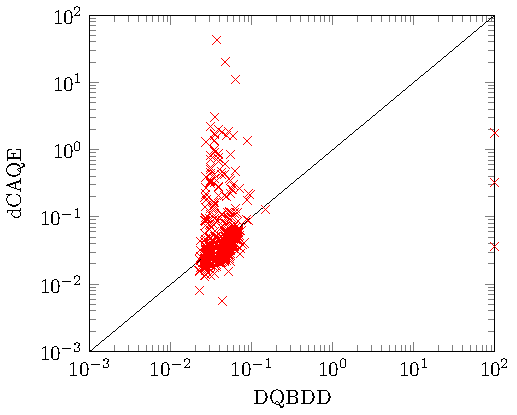
\includegraphics[width=\linewidth]{figures/PEC1dqbddVSdcaqe.pdf}
    \caption{DQBDD vs dCAQE for PEC1}
    \label{fig:PEC1dqbddVSdcaqe}
  \end{subfigure}
  \begin{subfigure}{0.48\textwidth}
    \centering
    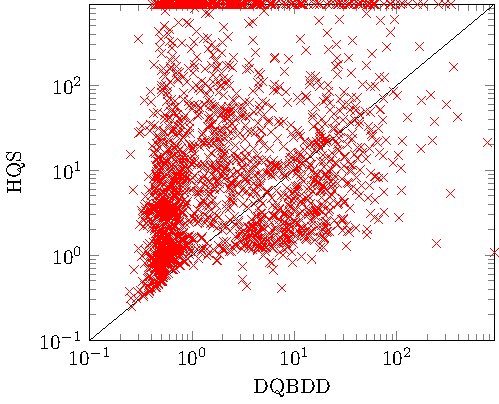
\includegraphics[width=\linewidth]{figures/PEC2dqbddVShqs.pdf}
    \caption{DQBDD vs HQS for PEC2}
    \label{fig:PEC2dqbddVShqs}
  \end{subfigure}
  \begin{subfigure}{0.48\textwidth}
    \centering
    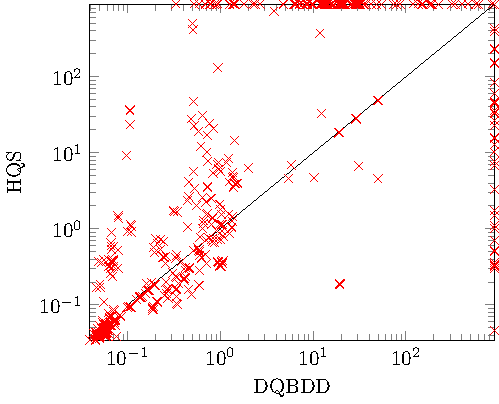
\includegraphics[width=\linewidth]{figures/PEC3dqbddVShqs.pdf}
    \caption{DQBDD vs HQS for PEC3}
    \label{fig:PEC3dqbddVShqs}
  \end{subfigure}
  \begin{subfigure}{0.48\textwidth}
    \centering
    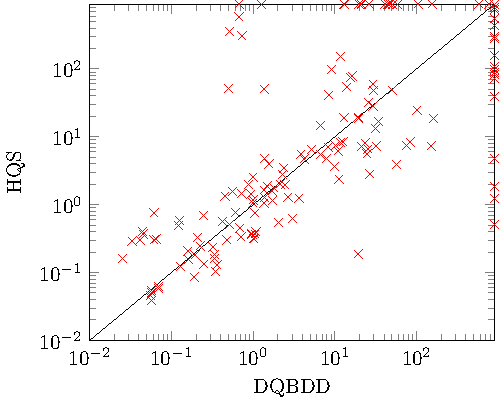
\includegraphics[width=\linewidth]{figures/E19dqbddVShqs.pdf}
    \caption{DQBDD vs HQS for E19}
    \label{fig:E19dqbddVShqs}
  \end{subfigure}
  \begin{subfigure}{0.48\textwidth}
    \centering
    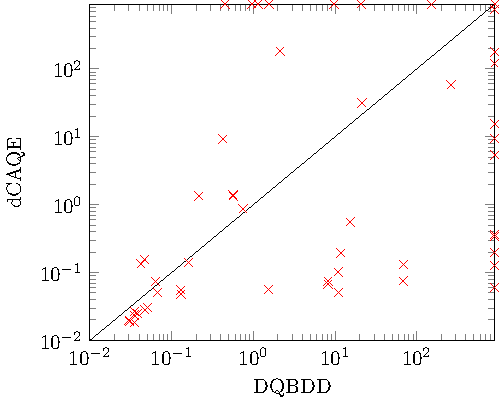
\includegraphics[width=\linewidth]{figures/CSPdqbddVSdcaqe.pdf}
    \caption{DQBDD vs dCAQE for CSP}
    \label{fig:CSPdqbddVSdcaqe}
  \end{subfigure}
  \begin{subfigure}{0.48\textwidth}
    \centering
    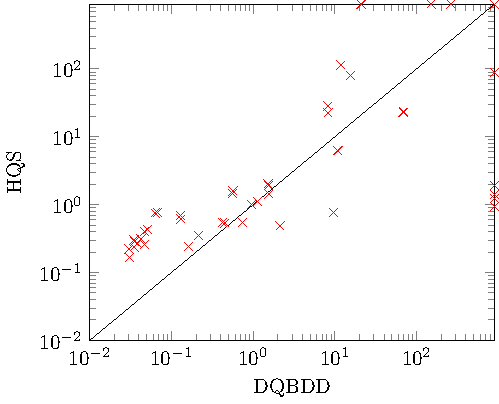
\includegraphics[width=\linewidth]{figures/CSPdqbddVShqs.pdf}
    \caption{DQBDD vs HQS for CSP}
    \label{fig:CSPdqbddVShqs}
  \end{subfigure}
  \caption{Comparison of solving times in seconds}
  \label{fig:runtimecomp}
\end{figure}

\begin{figure}
  \centering
  \begin{subfigure}{0.98\textwidth}
    \centering
    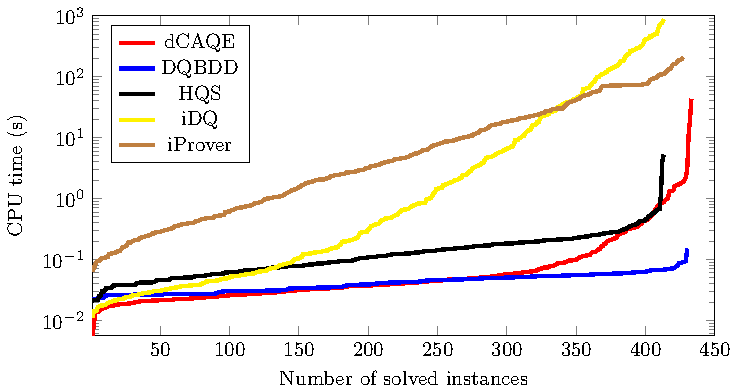
\includegraphics[width=\textwidth]{figures/PEC1logcactusplot.pdf}
    \caption{PEC1}
    \label{fig:cactusPEC1}
  \end{subfigure}
  \begin{subfigure}{0.98\textwidth}
    \centering
    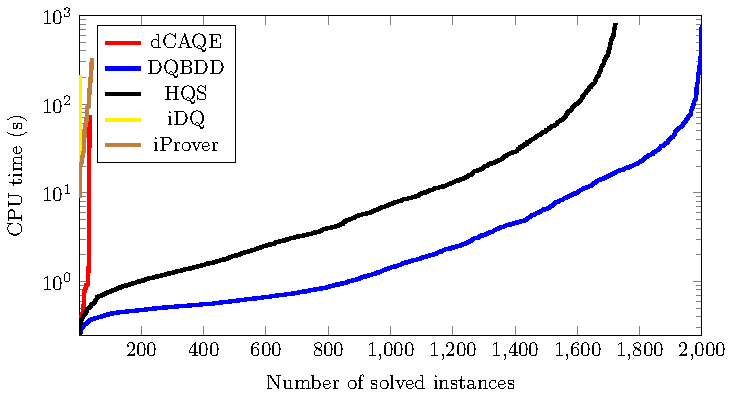
\includegraphics[width=\textwidth]{figures/PEC2logcactusplot.pdf}
    \caption{PEC2}
    \label{fig:cactusPEC2}
  \end{subfigure}
  \caption{Cactus plots for PEC1 and PEC2}
  \label{fig:cactusPEC12}
\end{figure}

\subsection{PEC1}

\begin{table}[t]
\centering
\caption{Comparison of solvers for PEC1 benchmark set}% with the total number of solved instances (\textbf{\#}) and the time taken to solve them, the number of solved satisfiable (\textbf{S}), unsatisfiable (\textbf{U}), and unique~(\textbf{*}) instances and the number of unsolved instances broken down to those that reached the time (\textbf{T}) or memory limit (\textbf{M}), or ended prematurely for some other reason (\textbf{O}).}
\label{tab:PEC1}
\begin{tabular}{|l|r|r|r|r|r|r|r|r|}
\hline
\multicolumn{1}{|c|}{}                                  & \multicolumn{5}{c|}{\textbf{Solved}}                                                                                                                                        & \multicolumn{3}{c|}{\textbf{Unsolved}}                                                                 \\  \hhline{~*{8}{-}}
\multicolumn{1}{|c|}{\multirow{-2}{*}{\textbf{Solver}}} & \multicolumn{1}{c|}{\textbf{\#}} & \multicolumn{1}{c|}{\textbf{Time (s)}} & \multicolumn{1}{c|}{\textbf{S}} & \multicolumn{1}{c|}{\textbf{U}} & \multicolumn{1}{c|}{\textbf{*}} & \multicolumn{1}{c|}{\textbf{T}} & \multicolumn{1}{c|}{\textbf{M}} & \multicolumn{1}{c|}{\textbf{O}} \\ \hline
\textbf{dCAQE} & \textbf{433} & \num{134.89} & \textbf{48} & \textbf{385} & \num{0} & \num{0} & \num{0} & \num{0} \\ \hline
\textbf{DQBDD} & \num{430} & \num{18.38} & \num{47} & \num{383} & \num{0} & \num{0} & \num{3} & \num{0} \\ \hline
\textbf{HQS} & \num{413} & \num{68.06} & \num{44} & \num{369} & \num{0} & \num{2} & \num{0} & \num{18} \\ \hline
\textbf{iDQ} & \num{413} & \num{16943.53} & \num{40} & \num{373} & \num{0} & \num{20} & \num{0} & \num{0} \\ \hline
\textbf{iProver} & \num{427} & \num{9118.53} & \num{43} & \num{384} & \num{0} & \num{6} & \num{0} & \num{0} \\ \hline
\end{tabular}
\end{table}

Table~\ref{tab:PEC1} shows the comparison of all solvers for PEC1 benchmarks which were not solved by HQSpre. All solvers solved most of the instances, while dCAQE solved \emph{all} 433 instances. This is followed by DQBDD and iProver which did not solve only three or six instances respectively. For the three instances that DQBDD did not solve, it reached the memory limit during quantifier localisation. Furthermore, the total runtime of DQBDD for solved instances is seven times less than dCAQE which in turn is 67 times less than iProver. On average, this means that it took DQBDD \SI{0.04}{s} to solve one instance while dCAQE took \SI{0.31}{s} and iProver took \SI{31.25}{s} per instance. The comparison of solving times for DQBDD and dCAQE is shown in Figure~\ref{fig:PEC1dqbddVSdcaqe}.

The remaining two solvers -- HQS and iDQ -- solved 413 instances each where HQS was 249 times faster than iDQ. Also notice that even though HQS solved less instances than DQBDD, DQBDD total runtime was still significantly smaller than HQS total runtime.

\subsection{PEC2}
The comparison of all solvers on all 2000 benchmarks from PEC2 benchmark set (as none of them were solved by HQSpre) is shown in Table~\ref{tab:PEC2}. Here, dCAQE, iDQ and iProver solved just a few instances whereas DQBDD and HQS solved most of them. For DQBDD, there was only one unsolved instance (caused by reaching memory limit during quantifier localisation) while HQS did not solve 278. Even with this, DQBDD was still more than twice as fast compared with HQS. Figure~\ref{fig:PEC2dqbddVShqs} shows the comparison of solving times of DQBDD and HQS.

The success of DQBDD and HQS for this benchmark set could be explained by gate extraction as explained in Section~\ref{sec:preprocessing} which simplifies input formulas. This stems from the fact that PEC problems encode circuits, which means there are possibly many gates to extract which can result in much more simplified formula compared to the formula in PCNF.

\begin{table}[ht]
\centering
\caption{Comparison of solvers for PEC2 benchmark set}% with the total number of solved instances (\textbf{\#}) and the time taken to solve them, the number of solved satisfiable (\textbf{S}), unsatisfiable (\textbf{U}), and unique~(\textbf{*}) instances and the number of unsolved instances broken down to those that reached the time (\textbf{T}) or memory limit (\textbf{M}), or ended prematurely for some other reason (\textbf{O}).}
\label{tab:PEC2}
\begin{tabular}{|l|r|r|r|r|r|r|r|r|}
\hline
\multicolumn{1}{|c|}{}                                  & \multicolumn{5}{c|}{\textbf{Solved}}                                                                                                                                        & \multicolumn{3}{c|}{\textbf{Unsolved}}                                                                 \\  \hhline{~*{8}{-}}
\multicolumn{1}{|c|}{\multirow{-2}{*}{\textbf{Solver}}} & \multicolumn{1}{c|}{\textbf{\#}} & \multicolumn{1}{c|}{\textbf{Time (s)}} & \multicolumn{1}{c|}{\textbf{S}} & \multicolumn{1}{c|}{\textbf{U}} & \multicolumn{1}{c|}{\textbf{*}} & \multicolumn{1}{c|}{\textbf{T}} & \multicolumn{1}{c|}{\textbf{M}} & \multicolumn{1}{c|}{\textbf{O}} \\ \hline
\textbf{dCAQE} & \num{34} & \num{134.12} & \num{0} & \num{34} & \num{0} & \num{1961} & \num{5} & \num{0} \\ \hline
\textbf{DQBDD} & \textbf{1999} & \num{19618.36} & \textbf{123} & \textbf{1876} & \textbf{278} & \num{0} & \num{1} & \num{0} \\ \hline
\textbf{HQS} & \num{1722} & \num{51769.75} & \num{80} & \num{1642} & \num{1} & \num{246} & \num{0} & \num{32} \\ \hline
\textbf{iDQ} & \num{4} & \num{292.66} & \num{0} & \num{4} & \num{0} & \num{1996} & \num{0} & \num{0} \\ \hline
\textbf{iProver} & \num{41} & \num{3382.37} & \num{1} & \num{40} & \num{0} & \num{9} & \num{1950} & \num{0} \\ \hline
\end{tabular}
\end{table}

\begin{figure}
  \centering
  \begin{subfigure}{0.98\textwidth}
    \centering
    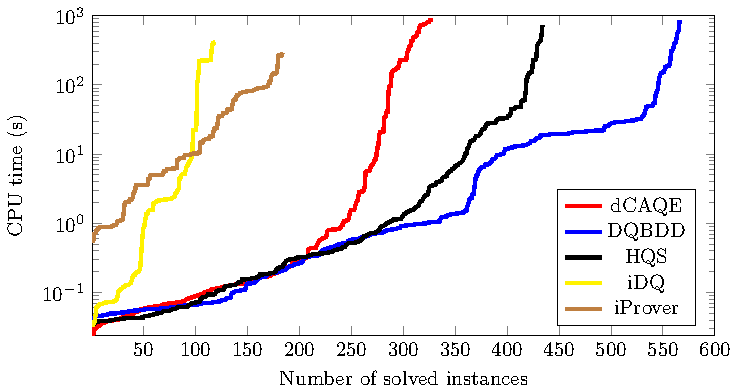
\includegraphics[width=\textwidth]{figures/PEC3logcactusplot.pdf}
    \caption{PEC3}
    \label{fig:cactusPEC3}
  \end{subfigure}
  \begin{subfigure}{0.98\textwidth}
    \centering
    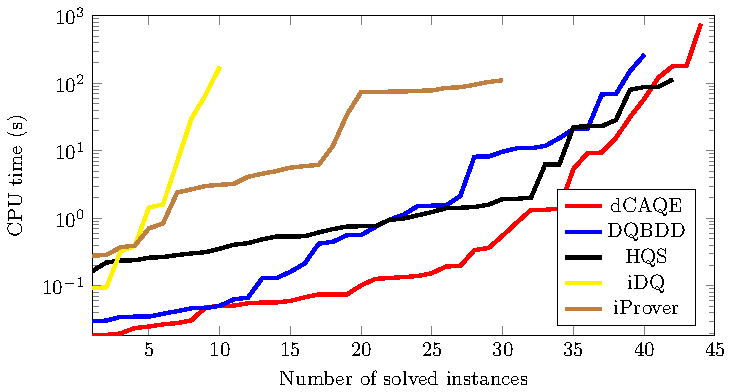
\includegraphics[width=\textwidth]{figures/CSPlogcactusplot.pdf}
    \caption{CSP}
    \label{fig:cactusCSP}
  \end{subfigure}
  \caption{Cactus plots for PEC3 and CSP}
  \label{fig:cactusPEC3CSP}
\end{figure}

\subsection{PEC3}
The results for the last PEC benchmark set are shown in Table~\ref{tab:PEC3}. Again, DQBDD and HQS solved the most instances (possibly because of gate extraction) followed by dCAQE, iProver, and finally by iDQ. Furthermore, DQBDD solved \num{132} instances more than HQS, where DQBDD took on average \SI{18.19}{s} per instance while HQS took \SI{15.73}{s}. Figure~\ref{fig:PEC3dqbddVShqs} shows the comparison of their runtimes for this benchmark set.

In this benchmark there were also three discrepancies: dCAQE solved three instances as satisfiable while HQS or DQBDD solved them as unsatisfiable (each solved two of them; iDQ and iProver did not solve them). This cannot be explained by the erroneous implementation of quantifier localisation in HQS because it can only turn unsatisfiable formulas to satisfiable ones. As both HQS and DQBDD use similar techniques for solving, it is hard to tell whether there is a mistake in dCAQE or HQS and DQBDD. However, as we show in Appendix~\ref{appendix:wrongdcaqe}, we can find a simple unsatisfiable DQBF which dCAQE determines as satisfiable. Also, because dCAQE works with the result of HQSpre without gate extraction and both HQS and DQBDD work with the result with gate extraction, the mistake could also be in HQSpre. However, we tried running all three instances using DQBDD with only the preprocessing without gate extraction and it determined all three as unsatisfiable, therefore we dismiss the possibility of mistake in HQSpre. This is why we believe that these instances are unsatisfiable and dCAQE solved them incorrectly.

\begin{table}[ht]
\centering
\caption{Comparison of solvers for PEC3 benchmark set}% with the total number of solved instances (\textbf{\#}) and the time taken to solve them, the number of solved satisfiable (\textbf{S}), unsatisfiable (\textbf{U}), and unique~(\textbf{*}) instances and the number of unsolved instances broken down to those that reached the time (\textbf{T}) or memory limit (\textbf{M}), or ended prematurely for some other reason (\textbf{O}).}
\label{tab:PEC3}
\begin{tabular}{|l|r|r|r|r|r|r|r|r|}
\hline
\multicolumn{1}{|c|}{}                                  & \multicolumn{5}{c|}{\textbf{Solved}}                                                                                                                                        & \multicolumn{3}{c|}{\textbf{Unsolved}}                                                                 \\  \hhline{~*{8}{-}}
\multicolumn{1}{|c|}{\multirow{-2}{*}{\textbf{Solver}}} & \multicolumn{1}{c|}{\textbf{\#}} & \multicolumn{1}{c|}{\textbf{Time (s)}} & \multicolumn{1}{c|}{\textbf{S}} & \multicolumn{1}{c|}{\textbf{U}} & \multicolumn{1}{c|}{\textbf{*}} & \multicolumn{1}{c|}{\textbf{T}} & \multicolumn{1}{c|}{\textbf{M}} & \multicolumn{1}{c|}{\textbf{O}} \\ \hline
\textbf{dCAQE} & \num{328} & \num{19271.73} & \num{96} & \num{232} & \num{3} & \num{565} & \num{0} & \num{0} \\ \hline
\textbf{DQBDD} & \textbf{566} & \num{10293.71} & \textbf{193} & \textbf{373} & \textbf{169} & \num{222} & \num{105} & \num{0} \\ \hline
\textbf{HQS} & \num{434} & \num{6825.99} & \num{142} & \num{292} & \num{29} & \num{444} & \num{0} & \num{15} \\ \hline
\textbf{iDQ} & \num{119} & \num{4778.43} & \num{39} & \num{80} & \num{4} & \num{774} & \num{0} & \num{0} \\ \hline
\textbf{iProver} & \num{184} & \num{6769.89} & \num{55} & \num{129} & \num{0} & \num{8} & \num{701} & \num{0} \\ \hline
\end{tabular}
\end{table}

\subsection{CSP}
Table~\ref{tab:CSP} shows the results for CSP benchmark set. For these, dCAQE, DQBDD, and HQS solved comparatively many instances (with dCAQE the most) while iProver and iDQ solved less. From those three, HQS was on average the fastest, spending \SI{12.01}{s} per instances, followed by DQBDD which spent \SI{17.05}{s} per instance. dCAQE was around two times slower than these two, taking on average \SI{31.21}{s} per instance. However, dCAQE runtime is dominated by one instance which took \SI{753.81}{s} to solve and was not solved by other solvers. If we remove this instance, dCAQE took on average \SI{14.41}{s}. Figures~\ref{fig:CSPdqbddVSdcaqe} and \ref{fig:CSPdqbddVShqs} show solving time comparison of DQBDD with dCAQE and HQS respectively.

\begin{table}[ht]
\centering
\caption{Comparison of solvers for CSP benchmark set}% with the total number of solved instances (\textbf{\#}) and the time taken to solve them, the number of solved satisfiable (\textbf{S}), unsatisfiable (\textbf{U}), and unique~(\textbf{*}) instances and the number of unsolved instances broken down to those that reached the time (\textbf{T}) or memory limit (\textbf{M}), or ended prematurely for some other reason (\textbf{O}).}
\label{tab:CSP}
\begin{tabular}{|l|r|r|r|r|r|r|r|r|}
\hline
\multicolumn{1}{|c|}{}                                  & \multicolumn{5}{c|}{\textbf{Solved}}                                                                                                                                        & \multicolumn{3}{c|}{\textbf{Unsolved}}                                                                 \\  \hhline{~*{8}{-}}
\multicolumn{1}{|c|}{\multirow{-2}{*}{\textbf{Solver}}} & \multicolumn{1}{c|}{\textbf{\#}} & \multicolumn{1}{c|}{\textbf{Time (s)}} & \multicolumn{1}{c|}{\textbf{S}} & \multicolumn{1}{c|}{\textbf{U}} & \multicolumn{1}{c|}{\textbf{*}} & \multicolumn{1}{c|}{\textbf{T}} & \multicolumn{1}{c|}{\textbf{M}} & \multicolumn{1}{c|}{\textbf{O}} \\ \hline
\textbf{dCAQE} & \textbf{44} & \num{1373.30} & \textbf{44} & \num{0} & \textbf{9} & \num{378} & \num{0} & \num{0} \\ \hline
\textbf{DQBDD} & \num{40} & \num{681.86} & \num{40} & \num{0} & \num{2} & \num{334} & \num{48} & \num{0} \\ \hline
\textbf{HQS} & \num{42} & \num{504.51} & \num{42} & \num{0} & \num{1} & \num{82} & \num{0} & \num{298} \\ \hline
\textbf{iDQ} & \num{10} & \num{281.18} & \num{10} & \num{0} & \num{0} & \num{407} & \num{5} & \num{0} \\ \hline
\textbf{iProver} & \num{30} & \num{1032.42} & \num{30} & \num{0} & \num{0} & \num{0} & \num{392} & \num{0} \\ \hline
\end{tabular}
\end{table}


\subsection{SAT}
The results for SAT benchmark set are in Table~\ref{tab:SAT}. This set consists of only few instances, therefore the comparison is not very interesting. However, we can see that DQBDD did not solve any formula from this set. This was caused by either not even finishing creation of the quantifier tree (three cases where DQBDD reached the memory limit) or getting stuck while creating the BDD (the cases where DQBDD reached the time limit). This benchmark therefore shows, that BDDs can sometime suffer from scalability problems.

\begin{table}[ht]
\centering
\caption{Comparison of solvers for SAT benchmark set}% with the total number of solved instances (\textbf{\#}) and the time taken to solve them, the number of solved satisfiable (\textbf{S}), unsatisfiable (\textbf{U}), and unique~(\textbf{*}) instances and the number of unsolved instances broken down to those that reached the time (\textbf{T}) or memory limit (\textbf{M}), or ended prematurely for some other reason (\textbf{O}).}
\label{tab:SAT}
\begin{tabular}{|l|r|r|r|r|r|r|r|r|}
\hline
\multicolumn{1}{|c|}{}                                  & \multicolumn{5}{c|}{\textbf{Solved}}                                                                                                                                        & \multicolumn{3}{c|}{\textbf{Unsolved}}                                                                 \\  \hhline{~*{8}{-}}
\multicolumn{1}{|c|}{\multirow{-2}{*}{\textbf{Solver}}} & \multicolumn{1}{c|}{\textbf{\#}} & \multicolumn{1}{c|}{\textbf{Time (s)}} & \multicolumn{1}{c|}{\textbf{S}} & \multicolumn{1}{c|}{\textbf{U}} & \multicolumn{1}{c|}{\textbf{*}} & \multicolumn{1}{c|}{\textbf{T}} & \multicolumn{1}{c|}{\textbf{M}} & \multicolumn{1}{c|}{\textbf{O}} \\ \hline
\textbf{dCAQE} & \num{7} & \num{2141.37} & \num{3} & \num{4} & \num{0} & \num{15} & \num{0} & \num{0} \\ \hline
\textbf{DQBDD} & \num{0} & \num{0} & \num{0} & \num{0} & \num{0} & \num{19} & \num{3} & \num{0} \\ \hline
\textbf{HQS} & \num{7} & \num{3030.71} & \textbf{5} & \num{2} & \textbf{2} & \num{15} & \num{0} & \num{0} \\ \hline
\textbf{iDQ} & \textbf{9} & \num{2546.24} & \num{4} & \textbf{5} & \num{1} & \num{13} & \num{0} & \num{0} \\ \hline
\textbf{iProver} & \num{8} & \num{3260.57} & \num{3} & \textbf{5} & \num{0} & \num{14} & \num{0} & \num{0} \\ \hline
\end{tabular}
\end{table}

\begin{figure}
  \centering
  \begin{subfigure}{0.98\textwidth}
    \centering
    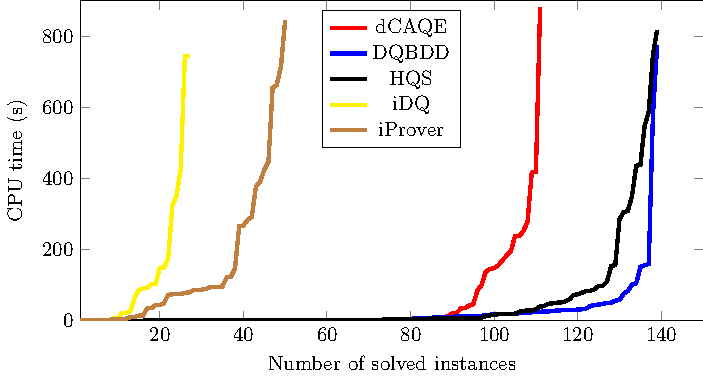
\includegraphics[width=\textwidth]{figures/E19cactusplot.pdf}
    \caption{PEC1}
    \label{fig:cactusPEC1}
  \end{subfigure}
  \begin{subfigure}{0.98\textwidth}
    \centering
    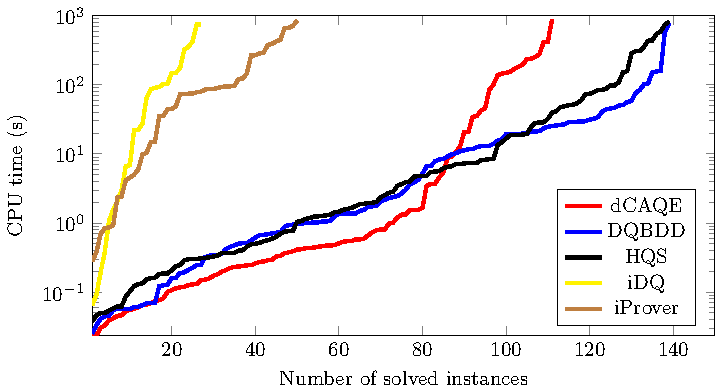
\includegraphics[width=\textwidth]{figures/E19logcactusplot.pdf}
    \caption{PEC2}
    \label{fig:cactusPEC2}
  \end{subfigure}
  \caption{Cactus plots for PEC1 and PEC2}
  \label{fig:cactusPEC12}
\end{figure}

\subsection{E19}
Finally, Table~\ref{tab:E19} shows the comparison of solvers for E19 benchmark set. As this set is a combination of previous sets (with also some new benchmarks), it is the most interesting for ``real'' comparison. However, this set is still dominated by PEC benchmarks, which shows up in the results: both DQBDD and HQS solved the most benchmarks, with 139 each (see Figure~\ref{fig:E19dqbddVShqs} for their runtime comparison). This is followed by dCAQE which solved 111 instances, then iProver with 50 instances, and finally iDQ with only 27 instances. Even though DQBDD solved the most, it was still the fastest, taking only \SI{3440.76}{s} for all of its solved instances. On average, this is \SI{24.75}{s} per instance, where dCAQE took \SI{39.06}{s} per instance, HQS took \SI{48.9}{s}, iDQ took \SI{136.97}{s} and iProver \SI{149.8}{s}.

There was also a discrepancy in this benchmark set. One instance, which is not in other benchmark sets, was deemed satisfiable by dCAQE while HQS claimed its unsatisfiability. Again, we believe that dCAQE solved it incorrectly.

\begin{table}[ht]
\centering
\caption{Comparison of solvers for E19 benchmark set}% with the total number of solved instances (\textbf{\#}) and the time taken to solve them, the number of solved satisfiable (\textbf{S}), unsatisfiable (\textbf{U}), and unique~(\textbf{*}) instances and the number of unsolved instances broken down to those that reached the time (\textbf{T}) or memory limit (\textbf{M}), or ended prematurely for some other reason (\textbf{O}).}
\label{tab:E19}
\begin{tabular}{|l|r|r|r|r|r|r|r|r|}
\hline
\multicolumn{1}{|c|}{}                                  & \multicolumn{5}{c|}{\textbf{Solved}}                                                                                                                                        & \multicolumn{3}{c|}{\textbf{Unsolved}}                                                                 \\  \hhline{~*{8}{-}}
\multicolumn{1}{|c|}{\multirow{-2}{*}{\textbf{Solver}}} & \multicolumn{1}{c|}{\textbf{\#}} & \multicolumn{1}{c|}{\textbf{Time (s)}} & \multicolumn{1}{c|}{\textbf{S}} & \multicolumn{1}{c|}{\textbf{U}} & \multicolumn{1}{c|}{\textbf{*}} & \multicolumn{1}{c|}{\textbf{T}} & \multicolumn{1}{c|}{\textbf{M}} & \multicolumn{1}{c|}{\textbf{O}} \\ \hline
\textbf{dCAQE} & \num{111} & \num{4335.81} & \num{37} & \num{74} & \num{1} & \num{135} & \num{0} & \num{0} \\ \hline
\textbf{DQBDD} & \textbf{139} & \num{3440.76} & \num{43} & \textbf{96} & \textbf{14} & \num{90} & \num{17} & \num{0} \\ \hline
\textbf{HQS} & \textbf{139} & \num{6796.64} & \textbf{51} & \num{88} & \num{5} & \num{53} & \num{0} & \num{54} \\ \hline
\textbf{iDQ} & \num{27} & \num{3698.26} & \num{13} & \num{14} & \num{1} & \num{218} & \num{1} & \num{0} \\ \hline
\textbf{iProver} & \num{50} & \num{7490.16} & \num{23} & \num{27} & \num{0} & \num{17} & \num{179} & \num{0} \\ \hline
\end{tabular}
\end{table}

%\subsection{Results Discussion???}

\chapter{Conclusion}
In this thesis, we have proposed and implemented a DQBF solver DQBDD that uses binary decision diagrams as an underlying representation of formulas. This solver is based on quantifier elimination and uses quantifier localisation which we have corrected and enhanced by adding a possibility to eliminate universal variables in subformulas.

Additionally, we experimentally evaluated different heuristics used in DQBDD and compared the best one with other DQBF solvers. We have shown that DQBDD performs very well, especially for partial equivalence checking problem.

\section{Future Work}

For future work there are multiple things possible to do:
\begin{itemize}
  \item We are planning to evaluate the impact of ordering of variables in BDDs. We can check whether it would make sense to set up some initial ordering and to decide what this ordering should be. We are also planning to try different reordering techniques used for BDDs, especially those that are already implemented in CUDD. They can be used dynamically, as we do now, but we can also gauge whether it is not better to decide when exactly we should reorder the variables in the algorithm.
  \item Another line of thinking would be to somehow combine HQS and DQBDD, similarly how it is done in QBF solver AIGSol\-ve~\cite{AIGSolve}. This solver uses mainly AIGs to represent the matrix of the formula, but during quantifier elimination, it can be turned into BDD with some size limit. If this BDD is created, quantifier elimination is done on it (as it is faster for BDDs than for AIGs) and then returned back to AIG, otherwise quantifier elimination is done directly on AIG. We could also use AIG or some similar structure during the localisation phase, where DQBDD sometimes hits the memory limit. This structure would reuse subtrees representing the same subformula (reducing the memory usage), and they would be copied only if there are some variables being pushed into them. Similar structure is already used in HQS, called quantifier graph~\cite{HQSquantifierLocalisation}.
  \item We are also planning to use more preprocessing techniques, especially the QBF approximations as explained in Section~\ref{sec:prepro:approximations} and the check whether an input formula can be effectively transformed into QBF as explained in Section~\ref{sec:prepro:pspacesubclass}. For these, we could also use some state of the art QBF solver.
  \item Another possible direction is to implement the quantifier elimination of only those universal variables which result in QBF as is done in HQS and possibly design and implement a QBF solver using BDDs which could solve it.
\end{itemize}

\begingroup
\setlength{\emergencystretch}{8em}
\printbibliography[heading=bibintoc]
\endgroup

%\chapter{Inserting the index}
%After using the \verb"\makeindex" macro and loading the
%\texttt{makeidx} package that provides additional indexing
%commands, index entries can be created by issuing the \verb"\index"
%command. \index{dummy text|(}It is possible to create ranged index
%entries, which will encompass a span of text.\index{dummy text|)}
%To insert complex typographic material -- such as $\alpha$
%\index{alpha@$\alpha$} or \TeX{} \index{TeX@\TeX} --
%into the index, you need to specify a text string, which will
%determine how the entry will be sorted. It is also possible to
%create hierarchal entries. \index{vehicles!trucks}
%\index{vehicles!speed cars}

%index:
%  \makeatletter\thesis@blocks@clear\makeatother
%  \phantomsection %% Print the index and insert it into the
%  \addcontentsline{toc}{chapter}{\indexname} %% table of contents.
%  \printindex

\appendix %% Start the appendices.

\chapter{Documentation for DQBDD}
\label{appendix:DQBDD}
DQBDD is a dependency quantifier Boolean formula (DQBF) solver that uses binary decision diagrams (BDDs) as an underlying representation of formulas. It is written in \Cplusplus{} and it reads DQBFs encoded in \DQDIMACS{} format~\cite{iDQandDQDIMACS} for which it checks their satisfiability using quantifier elimination. The source codes with binaries can be found at \url{https://github.com/jurajsic/DQBDD}. 


\section{Dependencies}
There is no need to install any dependency, all of them are compiled with DQBDD. They are these:
\begin{itemize}
  \item antom\footnote{\url{https://projects.informatik.uni-freiburg.de/projects/antom}} -- SAT solver used in HQSpre,
  \item CUDD v3.0.0\footnote{\url{https://github.com/ivmai/cudd}}~\cite{CUDD} -- BDD library,
  \item cxxopts v2.2.0\footnote{\url{https://github.com/jarro2783/cxxopts}} -- argument parser
  \item Easylogging\texttt{++} v9.96.7\footnote{\url{https://github.com/zuhd-org/easyloggingpp}} -- \Cplusplus{} logger used in HQSpre,
  \item HQSpre\footnote{\url{https://abs.informatik.uni-freiburg.de/src/projects_view.php?projectID=21}}~\cite{HQSpreJournal} -- DQBF preprocessor,
  \item PicoSAT\footnote{\url{http://fmv.jku.at/picosat/}}~\cite{PicoSAT} -- SAT solver used in HQSpre.
\end{itemize}

\section{Installation}
To compile DQBDD, a \Cplusplus{} compiler supporting C++14 standard and CMake\footnote{\url{https://cmake.org/}} is needed.

\newpage
\noindent Execute
\begin{verbatim}

  mkdir Release
  cd Release
  cmake -DCMAKE_BUILD_TYPE=Release ..
  make

\end{verbatim}
to build DQBDD which will be located in \verb|Release/src/|.

\section{Usage}
Run DQBDD with
\begin{verbatim}

  DQBDD [OPTION...] <input file>

\end{verbatim}
where \verb|<input file>| should be formula to solve in DQDIMACS format. The possible options are
\begin{verbatim}

  -h, --help                    Print usage
  -v, --version                 Print the version number
  -l, --localise arg            Use quantifier tree with
                                localisation of
                                quantifiers (default: 1)
  -p, --preprocess arg          Use preprocessing
                                (default: 1)
  -e, --elimination-choice arg  Decide what to eliminate on 
                                each level of quantifier
                                tree during transformation
                                to formula (default: 1)
  -u, --uvar-choice             The heuristics by which the 
                                next universal variable for
                                elimination is chosen
                                (default: 0)
  -d, --dyn-reordering          Allow dynamic reordering of
                                variables in BDDs
                                (default: 1)

\end{verbatim}
where for \verb|--localise|, \verb|--preprocess| and \verb|--dyn-reordering| the arguments are 0 or 1 to turn off or on the corresponding option. The option \verb|--elimination-choice| is used only if we localise and then we have these possible arguments:
\begin{itemize}
    \item 0 -- nothing is eliminated (\QEnone{}),
    \item 1 -- simple quantifiers are eliminated (\QEsimple{}),
    \item 2 -- all possible quantifiers are eliminated (\QEall{}).
\end{itemize}
For the option \verb|--uvar-choice| we have:
\begin{itemize}
    \item 0 -- the order of the universal variables is set at beginning (\QUatbeginning{}),
    \item 1 -- the variable with the currently lowest number of dependencies is chosen (\QUcurrentlowest{}),
    \item 2 -- the order is based on the number of variables in conjuncts of universal expansion (\QUvarsinconjuncts{}).
\end{itemize}
If the formula is satisfiable, the return value is 10, otherwise it is 20.

\section{Examples}
Running DQBDD as
\begin{itemize}
  \item \verb|DQBDD file.dqdimacs|
\end{itemize}
solves the formula in \verb|file.dqdimacs| with the default settings,
\begin{itemize}
  \item \verb|DQBDD --preprocess 0 --dyn-reordering 0 file.dqdimacs|
\end{itemize}
solves the formula in \verb|file.dqdimacs| without running the preprocessor HQSpre first and without using dynamic reordering of variables in BDDs as implemented in CUDD,
\begin{itemize}
  \item \verb|DQBDD --localise 0 --uvar-choice 1 file.dqdimacs|
\end{itemize}
solves the formula in \verb|file.dqdimacs| without localising quantifiers (or creating quantifier tree) where the next universal variable for universal expansion is always the one that has the minimal number of dependent existential variables,
\begin{itemize}
  \item \verb|DQBDD --localise 1 --elimination-choice 2 file.dqdimacs|
\end{itemize}
solves the formula in \verb|file.dqdimacs| with localising quantifiers where it eliminates all universal and possible existential variables while creating the final BDD from the quantifier tree.

\section{Licence}
DQBDD is licenced under version 3 of GNU Lesser General Public License~\cite{lgplv3}.

\chapter{DQDIMACS Format}
\label{appendix:DQDIMACS}
In this appendix, we define rhe \DQDIMACS{} format~\cite{iDQandDQDIMACS}, which can represent DQBFs in PCNF. 

\section{Syntax}
The format is defined by this BNF grammar (based on the one for \texttt{QDIMACS} format~\cite{QDIMACS}):
\begin{verbatim}

<input> ::= <preamble> <prefix> <matrix> EOF

<preamble>      ::= [<comment_lines>] <problem_line>
<comment_lines> ::= <comment_line> <comment_lines> 
                   | <comment_line> 
<comment_line>  ::= c <text> EOL
<problem_line>  ::= p cnf <pnum> <pnum> EOL

<prefix>     ::= [<quant_sets>]
<quant_sets> ::= <quant_set> <quant_sets> | <quant_set>
<quant_set>  ::= <quantifier> <atom_set> 0 EOL
<quantifier> ::= e | a | d
<atom_set>   ::= <pnum> <atom_set> | <pnum>

<matrix>      ::= <clause_list>
<clause_list> ::= <clause> <clause_list> | <clause> 
<clause>      ::= <literal> <clause> | <literal> 0 EOL
<literal>     ::= <num>

<text>  ::= {A sequence of non-special ASCII characters}
<num>   ::= {A 32-bit signed integer different from 0}
<pnum>  ::= {A 32-bit signed integer greater than 0}

\end{verbatim}
where the terminal symbols \verb|EOL| and \verb|EOF| stand for the end-of-line and end-of-file markers respectively, \verb|[<expr>]| denotes that \verb|<expr>| is an optional expression, and concatenation of expressions has precedence over choice between expressions. Furthermore, we have these additional constraints:
\begin{itemize}
    \item The first \verb|<pnum>| in \verb|<problem_line>| corresponds to the maximal possible number of distinct atoms appearing in the prefix and in the matrix, i.e., all the members of the quantified sets and the absolute value of each literal in all the clauses is less than or equal to this number.
    \item The second \verb|<pnum>| in \verb|<problem_line>| corresponds to the number of clauses appearing in the matrix, i.e., the number of <clause> expressions which <matrix> is comprised of.
    \item Each atom in the prefix must appear in the matrix.
    \item It is not possible to have two \verb|<quant_set>| after each other, where both have \verb|a| or both have \verb|e| as \verb|<quantifier>|.
    \item The same atom cannot appear in the prefix more than once except for atoms occurring in the second and further place of \verb|atom_set| with \verb|d| as \verb|<quantifier>|. All these atoms have to appear somewhere before in the prefix in \verb|<quant_set>| with \verb|a| quantifier.
\end{itemize}

\section{Semantics}
The meaning behind \verb|prefix| is that atoms appearing with \verb|<quantifier>| equal to
\begin{itemize}
    \item \verb|a| are universally quantified variables,
    \item \verb|e| are existentially quantified variables where each of them is dependent on all universally quantified variables which already appeared before and 
    \item \verb|d| are an existential variable with universal variables in its dependency set, that is the first atom is the existential variable $y$ and all others are universal variables in the dependency set $D_y$.
\end{itemize}

The number $n$ in \verb|<literal>| represents either the variable $x_n$ if it is positive or $\neg x_n$ if it is negative. Furthermore, all variables which appear in the matrix but do not appear in the prefix are existentially quantified with empty dependency sets. 

Note, that \DQDIMACS{} is by removing \verb|d| quantifiers backwards compatible with \texttt{QDIMACS} (used for QBFs) format and by removing the whole prefix with \texttt{DIMACS} (used for BFs) format.

\section{An Example}
As an example, we have that
\begin{verbatim}

 c Simple example
 p cnf 5 2
 a 1 2 0
 e 3 0
 d 4 1 0
 -1 2 3 0
 -2 -4 5 0
 
\end{verbatim}
represents DQBF
\[\forall x_1 \forall  x_2 \exists x_3 (x_1, x_2) \exists x_4(x_1) \exists x_5(\emptyset) \itholds ((\neg x_1 \lor x_2 \lor x_3) \land (\neg x_2 \lor \neg x_4 \lor x_5)).\]

\chapter{DQBF Wrongly Solved by dCAQE}
\label{appendix:wrongdcaqe}
Solver dCAQE deems a DQBF, which in \DQDIMACS{} format has the form
\begin{verbatim}

 p cnf 8 9
 a 1 2 3 0
 e 4 5 0
 a 6 0
 d 7 6 0
 d 8 6 0
 -1  2 3  4  5           0
 -1  2 3 -4              0
 -1  2 3    -5     7     0
  1 -2 3  4  5           0
  1 -2 3 -4            8 0
  1 -2 3    -5           0
  1  2 3  4  5           0
  1  2 3 -4    -6  -7    0
  1  2 3    -5  6     -8 0
 
\end{verbatim}
is satisfiable. However, this formula is not satisfiable. This is because the first three clauses force $x_7$ to be true no matter what $x_6$ is evaluated to. The fourth to sixth clauses force $x_8$ to be true too. The last three clauses then say that $x_4$ and $x_5$ would need to be dependent on $x_6$, which is not the case.

Other solvers (DQBDD, HQS, iDQ, iProver, and also preprocessor HQSpre) correctly decide its unsatisfiability.

\end{document}
